% Options for packages loaded elsewhere
\PassOptionsToPackage{unicode}{hyperref}
\PassOptionsToPackage{hyphens}{url}
%
\documentclass[
]{book}
\usepackage{lmodern}
\usepackage{amssymb,amsmath}
\usepackage{ifxetex,ifluatex}
\ifnum 0\ifxetex 1\fi\ifluatex 1\fi=0 % if pdftex
  \usepackage[T1]{fontenc}
  \usepackage[utf8]{inputenc}
  \usepackage{textcomp} % provide euro and other symbols
\else % if luatex or xetex
  \usepackage{unicode-math}
  \defaultfontfeatures{Scale=MatchLowercase}
  \defaultfontfeatures[\rmfamily]{Ligatures=TeX,Scale=1}
\fi
% Use upquote if available, for straight quotes in verbatim environments
\IfFileExists{upquote.sty}{\usepackage{upquote}}{}
\IfFileExists{microtype.sty}{% use microtype if available
  \usepackage[]{microtype}
  \UseMicrotypeSet[protrusion]{basicmath} % disable protrusion for tt fonts
}{}
\makeatletter
\@ifundefined{KOMAClassName}{% if non-KOMA class
  \IfFileExists{parskip.sty}{%
    \usepackage{parskip}
  }{% else
    \setlength{\parindent}{0pt}
    \setlength{\parskip}{6pt plus 2pt minus 1pt}}
}{% if KOMA class
  \KOMAoptions{parskip=half}}
\makeatother
\usepackage{xcolor}
\IfFileExists{xurl.sty}{\usepackage{xurl}}{} % add URL line breaks if available
\IfFileExists{bookmark.sty}{\usepackage{bookmark}}{\usepackage{hyperref}}
\hypersetup{
  pdftitle={Experiment},
  pdfauthor={Nils Gustafsson \& Nils Holmberg},
  hidelinks,
  pdfcreator={LaTeX via pandoc}}
\urlstyle{same} % disable monospaced font for URLs
\usepackage{color}
\usepackage{fancyvrb}
\newcommand{\VerbBar}{|}
\newcommand{\VERB}{\Verb[commandchars=\\\{\}]}
\DefineVerbatimEnvironment{Highlighting}{Verbatim}{commandchars=\\\{\}}
% Add ',fontsize=\small' for more characters per line
\usepackage{framed}
\definecolor{shadecolor}{RGB}{248,248,248}
\newenvironment{Shaded}{\begin{snugshade}}{\end{snugshade}}
\newcommand{\AlertTok}[1]{\textcolor[rgb]{0.94,0.16,0.16}{#1}}
\newcommand{\AnnotationTok}[1]{\textcolor[rgb]{0.56,0.35,0.01}{\textbf{\textit{#1}}}}
\newcommand{\AttributeTok}[1]{\textcolor[rgb]{0.77,0.63,0.00}{#1}}
\newcommand{\BaseNTok}[1]{\textcolor[rgb]{0.00,0.00,0.81}{#1}}
\newcommand{\BuiltInTok}[1]{#1}
\newcommand{\CharTok}[1]{\textcolor[rgb]{0.31,0.60,0.02}{#1}}
\newcommand{\CommentTok}[1]{\textcolor[rgb]{0.56,0.35,0.01}{\textit{#1}}}
\newcommand{\CommentVarTok}[1]{\textcolor[rgb]{0.56,0.35,0.01}{\textbf{\textit{#1}}}}
\newcommand{\ConstantTok}[1]{\textcolor[rgb]{0.00,0.00,0.00}{#1}}
\newcommand{\ControlFlowTok}[1]{\textcolor[rgb]{0.13,0.29,0.53}{\textbf{#1}}}
\newcommand{\DataTypeTok}[1]{\textcolor[rgb]{0.13,0.29,0.53}{#1}}
\newcommand{\DecValTok}[1]{\textcolor[rgb]{0.00,0.00,0.81}{#1}}
\newcommand{\DocumentationTok}[1]{\textcolor[rgb]{0.56,0.35,0.01}{\textbf{\textit{#1}}}}
\newcommand{\ErrorTok}[1]{\textcolor[rgb]{0.64,0.00,0.00}{\textbf{#1}}}
\newcommand{\ExtensionTok}[1]{#1}
\newcommand{\FloatTok}[1]{\textcolor[rgb]{0.00,0.00,0.81}{#1}}
\newcommand{\FunctionTok}[1]{\textcolor[rgb]{0.00,0.00,0.00}{#1}}
\newcommand{\ImportTok}[1]{#1}
\newcommand{\InformationTok}[1]{\textcolor[rgb]{0.56,0.35,0.01}{\textbf{\textit{#1}}}}
\newcommand{\KeywordTok}[1]{\textcolor[rgb]{0.13,0.29,0.53}{\textbf{#1}}}
\newcommand{\NormalTok}[1]{#1}
\newcommand{\OperatorTok}[1]{\textcolor[rgb]{0.81,0.36,0.00}{\textbf{#1}}}
\newcommand{\OtherTok}[1]{\textcolor[rgb]{0.56,0.35,0.01}{#1}}
\newcommand{\PreprocessorTok}[1]{\textcolor[rgb]{0.56,0.35,0.01}{\textit{#1}}}
\newcommand{\RegionMarkerTok}[1]{#1}
\newcommand{\SpecialCharTok}[1]{\textcolor[rgb]{0.00,0.00,0.00}{#1}}
\newcommand{\SpecialStringTok}[1]{\textcolor[rgb]{0.31,0.60,0.02}{#1}}
\newcommand{\StringTok}[1]{\textcolor[rgb]{0.31,0.60,0.02}{#1}}
\newcommand{\VariableTok}[1]{\textcolor[rgb]{0.00,0.00,0.00}{#1}}
\newcommand{\VerbatimStringTok}[1]{\textcolor[rgb]{0.31,0.60,0.02}{#1}}
\newcommand{\WarningTok}[1]{\textcolor[rgb]{0.56,0.35,0.01}{\textbf{\textit{#1}}}}
\usepackage{longtable,booktabs}
% Correct order of tables after \paragraph or \subparagraph
\usepackage{etoolbox}
\makeatletter
\patchcmd\longtable{\par}{\if@noskipsec\mbox{}\fi\par}{}{}
\makeatother
% Allow footnotes in longtable head/foot
\IfFileExists{footnotehyper.sty}{\usepackage{footnotehyper}}{\usepackage{footnote}}
\makesavenoteenv{longtable}
\usepackage{graphicx}
\makeatletter
\def\maxwidth{\ifdim\Gin@nat@width>\linewidth\linewidth\else\Gin@nat@width\fi}
\def\maxheight{\ifdim\Gin@nat@height>\textheight\textheight\else\Gin@nat@height\fi}
\makeatother
% Scale images if necessary, so that they will not overflow the page
% margins by default, and it is still possible to overwrite the defaults
% using explicit options in \includegraphics[width, height, ...]{}
\setkeys{Gin}{width=\maxwidth,height=\maxheight,keepaspectratio}
% Set default figure placement to htbp
\makeatletter
\def\fps@figure{htbp}
\makeatother
\setlength{\emergencystretch}{3em} % prevent overfull lines
\providecommand{\tightlist}{%
  \setlength{\itemsep}{0pt}\setlength{\parskip}{0pt}}
\setcounter{secnumdepth}{5}
\usepackage[]{natbib}
\bibliographystyle{apalike}

\title{Experiment}
\author{Nils Gustafsson \& Nils Holmberg}
\date{2022-04-27}

\begin{document}
\maketitle

{
\setcounter{tocdepth}{1}
\tableofcontents
}
\hypertarget{part-del-1}{%
\part{Del 1}\label{part-del-1}}

\hypertarget{del-1}{%
\chapter*{Del 1}\label{del-1}}
\addcontentsline{toc}{chapter}{Del 1}

I denna del av boken följer vi utvecklingen och genomförandet av ett samhällsvetenskapligt experiment.

\hypertarget{chap01}{%
\chapter{Kapitel}\label{chap01}}

I denna del av boken följer vi utvecklingen och genomförandet av ett samhällsvetenskapligt experiment. Exempel på en \textbf{figur} kommer här:

\begin{figure}

{\centering 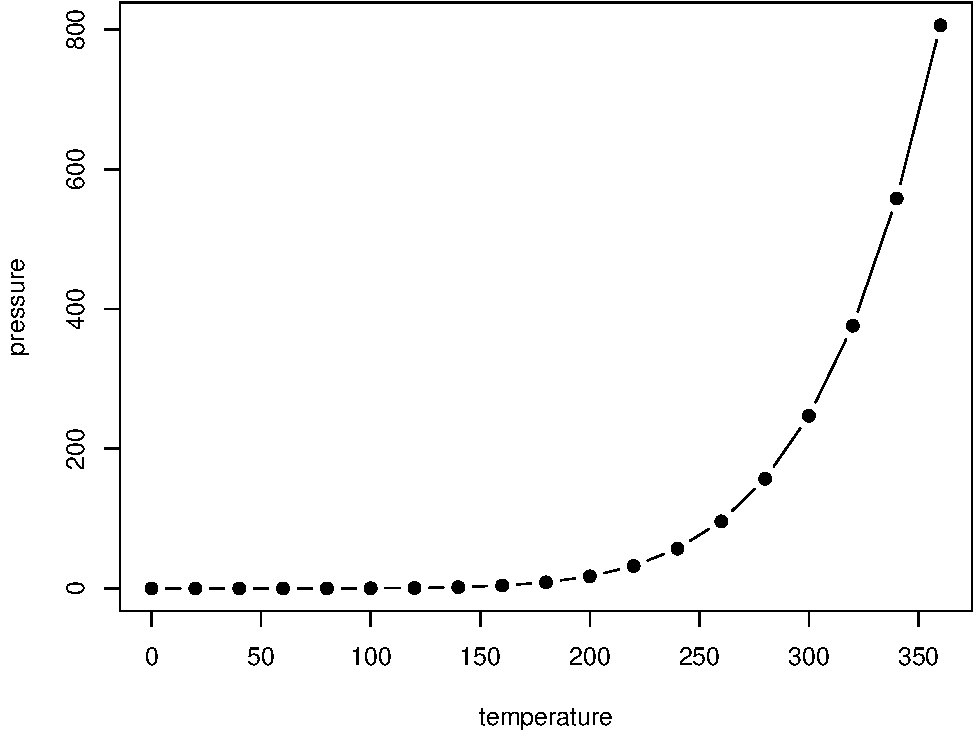
\includegraphics[width=0.8\linewidth]{scom-expb_files/figure-latex/fig01-01-1} 

}

\caption{En figur.}\label{fig:fig01-01}
\end{figure}

En linjär modell.

\begin{Shaded}
\begin{Highlighting}[]
\CommentTok{\# Predictor vs Criterion \{ggplot2\} {-} separate regression lines}
\NormalTok{gp =}\StringTok{ }\NormalTok{ggplot2}\OperatorTok{::}\KeywordTok{ggplot}\NormalTok{(}\DataTypeTok{data=}\NormalTok{iris, }
\NormalTok{ggplot2}\OperatorTok{::}\KeywordTok{aes}\NormalTok{(}\DataTypeTok{x=}\NormalTok{Sepal.Length,}
\DataTypeTok{y=}\NormalTok{Petal.Length,}
\DataTypeTok{colour=}\NormalTok{Species)) }\OperatorTok{+}\StringTok{ }
\NormalTok{ggplot2}\OperatorTok{::}\KeywordTok{geom\_smooth}\NormalTok{(}\DataTypeTok{method=}\NormalTok{lm) }\OperatorTok{+}\StringTok{ }
\NormalTok{ggplot2}\OperatorTok{::}\KeywordTok{geom\_point}\NormalTok{(}\DataTypeTok{size =} \DecValTok{2}\NormalTok{) }\OperatorTok{+}
\NormalTok{ggplot2}\OperatorTok{::}\KeywordTok{ggtitle}\NormalTok{(}\StringTok{"Sepal Length vs Petal Length"}\NormalTok{) }\OperatorTok{+}
\NormalTok{ggplot2}\OperatorTok{::}\KeywordTok{xlab}\NormalTok{(}\StringTok{"Sepal Length"}\NormalTok{) }\OperatorTok{+}\StringTok{ }\NormalTok{ggplot2}\OperatorTok{::}\KeywordTok{ylab}\NormalTok{(}\StringTok{"Petal Length"}\NormalTok{)}
\CommentTok{\#}
\KeywordTok{print}\NormalTok{(gp)}
\end{Highlighting}
\end{Shaded}

\begin{verbatim}
## `geom_smooth()` using formula 'y ~ x'
\end{verbatim}

\begin{figure}

{\centering 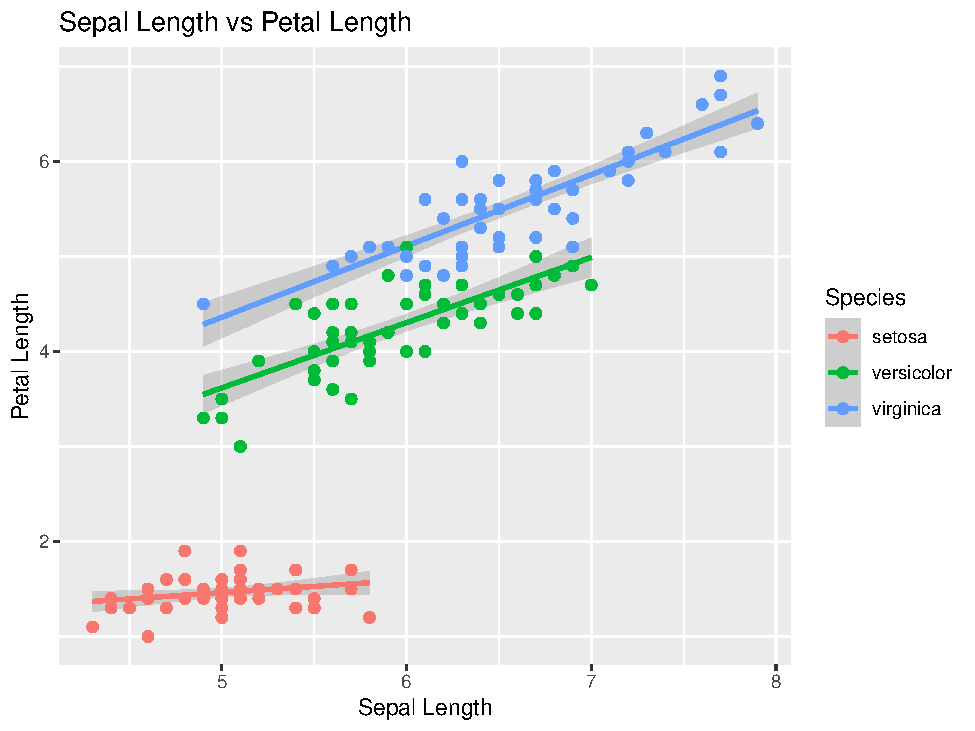
\includegraphics[width=0.8\linewidth]{scom-expb_files/figure-latex/fig01-02-1} 

}

\caption{Figur 1. Linjära modeller}\label{fig:fig01-02}
\end{figure}

\hypertarget{chap02}{%
\chapter{Kapitel}\label{chap02}}

I denna del av boken följer vi utvecklingen och genomförandet av ett samhällsvetenskapligt experiment. Exempel på en \textbf{tabell} kommer här:

\hypertarget{chap03}{%
\chapter{Kapitel}\label{chap03}}

I denna del av boken följer vi utvecklingen och genomförandet av ett samhällsvetenskapligt experiment. Exempel på en \textbf{referens} \citep{xie2015} kommer här.

\hypertarget{chap04}{%
\chapter{Kapitel}\label{chap04}}

I denna del av boken följer vi utvecklingen och genomförandet av ett samhällsvetenskapligt experiment.

\hypertarget{chap05}{%
\chapter{Kapitel}\label{chap05}}

I denna del av boken följer vi utvecklingen och genomförandet av ett samhällsvetenskapligt experiment.

\newpage

\hypertarget{part-del-2}{%
\part{Del 2}\label{part-del-2}}

\hypertarget{del-2}{%
\chapter*{Del 2}\label{del-2}}
\addcontentsline{toc}{chapter}{Del 2}

I denna del av boken följer vi utvecklingen och genomförandet av ett samhällsvetenskapligt experiment. Närmare bestämt kommer vi resonera kring ett tänkt experiment som tar avstamp inom kommunkationsforskningen, där man bland annat undersöker hur sociala medier såsom Facebook och Twitter används för att på olika sätt påverka mediepubliker. Till skillnad från den första delen av boken, där vi introducerade experiment som vetenskaplig metod, kommer del 2 att vara mer konkret och fokusera på de praktiska moment som ofta behöver beaktas i samband med planering, genomförande, och rapportering av ett experiment. Denna del av boken följer också ett kronologiskt upplägg, där vi börjar med att diskutera frågor som kommer tidigt i experiment-processen, och sedan övergår till att gå igenom praktiska frågor kring experimentets design. Vi kommer också använda oss av ett flertal andra konkreta experiment-exempel där detta krävs. Tanken med del 2 är att ge studenter ett ``matlagningsrecept'' för experimentella studier, där ``ingredienserna'' kan bytas ut och kombineras på nya sätt för att besvara nya frågeställningar. Vi är dock övertygade om att de flesta framgångsrika experiment följer vissa nödvändiga steg som successivt bygger på varandra. I denna bok kallat vi dessa steg för Förarbete (Kapitel 6), Genomförande (Kapitel 7), och Efterarbete (Kapitel 8).

\textbf{Förarbete.} I detta kapitel fokuserar vi på planeringsfasen i ett experiment. Denna fas är naturligtvis viktig oavsett vilken typ av studie vi ämnar genomföra, men på grund av att samhällsvetenskapliga experiment generellt sett vill undersöka hur en viss behandling påverkar människor, blir det avgörande att undersöka om och hur detta gjorts tidigare. Undersökningen av tidigare forskning tillåter oss att formulera (en eller flera) \emph{forskningsfrågor} som bygger vidare på tidigare forskningsresultat, och som därmed kan anses vara relevanta för forskningsfältet. När vi har formulerat forskningsfrågor med stöd av teoribildning och tidigare forskning har vi i nästa steg möjlighet att \emph{operationalisera} dessa frågor genom att omsätta kvalitativa begrepp till mätbara variabler. Detta steg kan vara så enkelt som att formulera en enkätfråga på ett sätt som visat sig vara framgångsrikt inom tidigare studier. När vi har operationaliserat forskningsfrågorna till mätbara variabler, kan vi åstadkomma den sista delen av förarbetet, i vilken vi formulerar \emph{hypoteser} om de statistiska samband vi förväntar oss att finna mellan våra mätvariabler. Allt detta förarbete till ett experiment är sådan information som ofta placeras i introduktionen till en uppsats eller forskningsartikel.

\textbf{Genomförande.} Detta kapitel behandlar de viktigaste praktiska stegen i experimentets genomförande. Dessa steg redovisas ofta utförligt i metoddelen av en uppsats eller forskningsartikel, och syftet med denna experimentbeskrivning är att möjliggöra upprepning av andra forskare. Genom att tidigt i forskningsprocessen göra ett \emph{pilottest} kan vi själva som forskare försäkra oss om att experimentet fungerar som vi har tänkt innan vi samlar in data. Därefter kommer den fullskaliga rekryteringen av \emph{försöksdeltagare} som nästa viktiga steg i genomförandet av ett experiment, och i detta steg är det viktigt att fundera på hur vi uppnår representativitet, samt hur vi rent praktiskt ska motivera personer att avsätta tid för att delta i studien och generera mätdata åt oss. När vi genomför ett experiment innebär det nästan alltid att vi använder någon form av \emph{mätinstrument} för att uppmäta hur våra försöksdeltagare svarar på en behandling. Denna behandling ingår i undersökningens \emph{experimentella villkor}, och tanken är ofta att konstrastera en uppmätt variabel mellan ett kontrollvillkor och ett behandlingsvillkor. Exakt hur varje deltagare genomgår dessa villkor definieras av den \emph{experimentella design} vi beslutat oss för att använda. När vi genomför experimentet är det viktigt att alla deltagare genomgår en standardiserad \emph{procedur} för att minska effekten av godtyckliga bruskällor i deltagarnas responser. Experimentets genomförande avslutas med \emph{dataanalys} som beskriver hur vi bearbetat mätvariablerna innan vi utvärderar effekten av våra experimentella villkor, vilket kommer att bli experimentents resultat.

\textbf{Efterarbete.} I detta kapitel tar vi upp: hur man kan redovisa resultatet av ett genomfört experiment, hur vi kan diskutera den samhälleliga och forskningsmässiga relevansen av undersökningen, samt hur resultaten kan rapporteras i form av en publicerad artikel. Naturligtvis förutsätter detta sista steg att vi klarat av de tidigare stegen. När vi är klara med själva genomförandet av ett experiment, brukar det första steget i efterarbetet vara att redovisa de \emph{resultat} undersökningen har lett fram till. Resultaten redovisas ofta i två steg, först med deskriptiva och sedan med inferentiella statistiska metoder. Den inferentiella statistiken används för att testa de hypoteser som inledningsvis uppställdes i förarbetet till experimentet, t.ex. att vi förväntade oss att hitta signifikanta skillnader mellan deltagarnas uppmätta responser i experimentets olika villkor. Efter att vi på detta sätt redovisat förhållandet mellan våra inledningsvis förväntade resultat och våra faktiska uppmätta resultat brukar man skriva en \emph{diskussion} om alternativa förklaringar till undersökningens observerade resultat, samt hur experimentet kan utvecklas och förbättras genom ytterligare forskning i framtiden. Avslutningsvis kommer detta kapitel diskutera vad forskare bör tänka på vid eventuell \emph{publicering} av forskningsresultat.

Genomgående försöker denna lärobok täcka in två olika men näraliggande betydelser av begreppet experimentell metod: dels som en uppsättning praktiska tillvägagångssätt som bör användas för att \emph{planera} och genomföra en experimentell studie; och dels som ett systematiskt och standardiserat sätt att i efterhand \emph{rapportera} genomförandet av en studie på ett sätt som är begripligt för andra forskare. Således är denna andra del av läroboken disponerat på ett sätt som ger oss möjlighet att i typisk turordning behandla de olika aspekter av experimentell metod som man som forskare förväntas kunna redovisa när man rapporterar sina resultat till en vetenskaplig tidskrift. Men inom varje metodaspekt kommer vi också att utförligt diskutera de olika experimentella tillvägagångssätt som är relevanta i samband med planering och genomförande av en forskningsstudie.

\hypertarget{chap06}{%
\chapter{Förarbete}\label{chap06}}

Innan man genomför ett experiment är det viktigt att noga undersöka om liknande experiment redan genomförts genom tidigare forskning. Inom samhällsvetenskapliga ämnen kan det exempelvis vara intressant att undersöka hur mediepublikers attityder, kunskaper och beteenden påverkas av olika typer av kommunikativa åtgärder (interventioner), t.ex. en marknadsföringskampanj eller ett politiskt budskap. På samma sätt är det inom medicinska vetenskaper ofta av intresse att utröna om ett nytt läkemedel har någon positiv effekt på patienter jämfört med en kur bestående av verkningslösa sockerpiller. Ju mer mån man är att undersöka ett tillförlitligt kausalt samband mellan en behandling och tillståndet hos målgrupp, desto viktigare blir det att kunna genomföra ett kontrollerat experiment, där effekterna av en behandling systematiskt jämförs med effekterna av en annan behandling (eller ingen behandling alls).

Det är inte ovanligt att en organisation som investerar pengar i en marknadsföringskampanj, också vill utvärdera olika kausala effekter av denna kommunikation på konsumenter. Genom att inventera tidigare forskningslitteratur inom detta specifika område, visar det sig ofta vilka mått och mätmetoder som använts, samt vad man kan förvänta sig om man genomför ett nytt experiment inom ett liknande experimentellt paradigm (REF). Framför allt kan tidigare forskning hjälpa oss att formulera några övergripande \emph{forskningsfrågor} som på något sätt för forskningsfältet framåt. Alla dessa aspekter av hur en ny, planerad studie förhåller sig till tidigare forskning, är viktiga genom hela forskningsprocessen. Tidigare använda mått och mätmetoder kan nämligen ge en god uppfattning om hur vi ska \emph{operationalisera} våra forskningsfrågor till mätbara variabler (mer om detta längre fram). Tidigare uppnådda resultat, å andra sidan, genererar vissa förväntningar om vilka resultat vårt eget experiment kommer att leda till, vilket i sin tur hjälper oss att formulera motiverade \emph{hypoteser} som är härledda från tidigare forskning inom området \citep{holmberg-2016-effects}.

Inom flera samhällsvetenskapliga discipliner har den konstruktivistiska kunskapssynen haft en framträdande roll under de senaste decennierna (ref). Som en konsekvens av detta har det blivit viktigt att ange en så kallad teoretisk referensram i samband med att man introducerar en kvalitativ forskningsstudie. Denna samling av teoretiska perspektiv (t.ex. retorisk eller semiotisk teoribildning) har sedan en viktig funktion vid analysen av empiriskt material, närmare bestämt genom att materialet tolkas med utgångspunkt i de teoretiska perspektiv man valt (därav den så kallade hermeneutiska forskningstraditionen). Inom den experimentella forskningen beskrivs kunskapssynen snarare som positivistisk, och teoretiska perspektiv används för att göra förutsägelser eller prediktioner om numeriska samband vi förväntar oss att hitta i kvantitiva mätdata. Detta gör att teorier generellt sett spelar en annan roll inom ett experiment jämfört med en kvalitativ studie, eftersom experiment använder empiriska resultat för att testa, och eventuellt uppdatera, befintlig teoribildning. Se även vetenskapsteori, Del 1.

När vi rapporterar förarbetet till ett experiment, görs detta ofta inom artikelns introduktion (jfr. akronymen IMRD i kapitel 8). När man introducerar en experimentell studie brukar man inleda med en kort bakgrund av det aktuella forskningsläget och en motivering till den genomförda undersökningen. Det är viktigt att det i ett tidigt skede står klart för läsaren vilket forskningsproblem (eller "kunskapsgap") studien vill bidra till att undersöka och helst råda bot på. Genomgången av tidigare forskning ska leda fram till och motivera den aktuella studiens forskningsfrågor och hypoteser. Det blir därmed viktigt att introduktionen och forskningsfrågorna refererar till empiriska resultat från tidigare forskning.

\hypertarget{sec06.1}{%
\section{Forskningsfrågor}\label{sec06.1}}

En viktig del av introduktionen till alla typer av vetenskapliga studier är att presentera studiens forskningsfrågor. Forskningsfrågor brukar i allmänhet vara nära kopplade till studiens syfte och mål, och bör därför vara möjliga att besvara inom ramen för studiens genomförande. Av denna anledning är forskningsfrågor ofta ganska generellt formulerade.

En forskningsfråga ska på ett någorlunda enkelt och kortfattat sätt sammanfatta vilka frågeställningar som ett specifikt experiment adresserar. Därför är det förhållandevis accepterat att forskningsfrågor är något abstrakt formulerade, så länge de ändå är enkla, lättfattliga och kortfattade. Introduktionens vidare uppgift är nämligen att konkretisera studiens forskningsfrågor genom en process som kallas \emph{operationalisering}, i vilken dessa forskningsfrågor omsätts till mätbara variabler som sedan kan ingå i falsifierbara \emph{hypoteser}. Man kan därför uttrycka det som att hypoteserna i en experimentell studie operationaliserar studiens forskningsfrågor. Operationalisering är ett mycket viktigt begrepp inom experimentell forskning, och vi återkommer mer utförligt till detta begrepp lite längre fram i detta kapitel, där vi också diskuterar hur detta begrepp hänger ihop med hypotesformulering.

Återgår vi till att diskutera begreppet forskningsfrågor mer generellt så finns det vissa tumregler som är viktiga att beakta. Den första tumregeln är att en forskningsfråga i någon del bör bygga på tidigare forskningsresultat, samt i någon del bör innehålla något nytt och outforskat. Med en sådan forskningsfråga kan man både upprepa (replikera) aspekter av tidigare forskning, men också utöka (extendera) tidigare forskning i syfte att skapa ny kunskap. En annan regel är att en forskningsfråga naturligtvis inte ska innehålla flera olika frågor, samt att två forskningsfrågor inte bör vara beroende av varandra (se övrig metodlitteratur, ref). Inom ramen för denna lärobok antar vi att en intressant forskningsfråga handlar om hur bildinnehållet i Facebook-poster påverkar läsarnas beteende och attityder. Närmare bestämt vill vi undersöka en upptäckt inom psykologisk forskning som visar att ett budskap upplevs som mer övertygande om det görs av en person som uppfattas som en auktoritet inom ett område (REF: Cialdini, 2001). Exempelvis kan vi föreslå att personen Leif GW Persson uppfattas som en auktoritet inom området kriminologi bland stora delar av den svenska mediepubliken. Vidare tänker vi oss att budskapet i en Facebook-post kan associeras med en auktoritetsperson genom att denna person visas i en bild som tillhör posten.

\hypertarget{sub06.1.1}{%
\subsection{Planering av forskningsfrågor}\label{sub06.1.1}}

I vårt tänkta experiment kretsar forskningsfrågorna kring effekterna av bildegenskaper hos Facebook-poster på internetanvändares visuella uppmärksamhet i samband med att de interagerar med dessa poster, samt effekter av bildinnehåll på användarnas självrapporterade nivå av upplevd trovärdighet hos samma poster. Låt oss anta att vi vill använda en av de sju ``principer för att övertyga'' som formulerats av den poplärvetenskapliga psykologiforskaren Robert Cialdini (\url{https://en.wikipedia.org/wiki/Robert_Cialdini}), närmare bestämt principen om auktoritet, och undersöka om en sådan intuition faktiskt verkar vara samstämmig med resultat från ett experiment som inkluderar fysiologiska mätmetoder såsom ögonrörelsemätning. ``Auktoritetsprincipen'' som vi fokuserar på här förutsäger att om ett budskap presenteras tillsammans med en person som är expert inom samma område så kommer mottagaren att uppleva detta budskap som mer trovärdigt. Personens auktoritet smittar så att säga av sig på det budskap någon försöker förmedla.

Vidare kan vi anta att vi har hittat tidigare forskning inom tidningsbranchen som undersökt hur bildsättning av nyhetsartiklar påverkar hur trovärdiga tidningsläsare upplever att dessa artiklar är. Forskningsfrågan tar alltså avstamp i något som i någon mån antas vara utforskat eller välkänt (prinipen om auktoritet och upplevd trovärdighet hos nyhetsartiklar), och utvidgar sedan undersökningen till något som är mindre utforskat (sociala medier-poster på Facebook och läsares visuella beteende).

\hypertarget{sub06.1.2}{%
\subsection{Rapportering av forskningsfrågor}\label{sub06.1.2}}

När man arbetar med ett manuskript för en artikel eller uppsats så formuleras ofta forskningsfrågorna som ``research questions'', vilket ibland förkortas RQ. En studie kan naturligtvis fokusera på flera relaterade forskningsfrågor, men det vanligaste är att man adresserar en eller två huvudfrågor, som sedan kan delas in ytterligare i underfrågor (RQ1a, osv). Exempel på formulerade forskningsfrågor med anknytning till bokens exempel-experiment. Således, i vårt tänkta experiment skulle den första forskningsfrågan kunna formuleras:

\begin{itemize}
\tightlist
\item
  RQ1: Hur påverkar bildinnehållet i sociala medier-poster användarnas beteenden och attityder?
\end{itemize}

Som underfrågor till denna forskningsfråga skulle man kunna tänka sig ``RQ1a: Hur påverkar bildinnehållet i Facebook-poster läsarnas blickbeteende'', och ``RQ1b: Hur påverkar bildinnehållet i Facebook-poster läsarnas attityder gällande postens trovärdighet''. Det är viktigt att här betona att det finns många olika sätt att formulera forskningsfrågor, och att det sätt vi föreslår här hänger nära samman med experiment i hög grad vill bygga vidare på tidigare forskning, men samtidigt belysa nya frågeställningar. Vi tror också att detta sätt formulera forskningsfrågor förenklar processen att omvandla dessa till hypoteser. (Vissa vetenskapliga tidskrifter har en mycket strikt tolkning av experimentell metod, vilket innebär att hypoteserna i ett så kallat naturligt experiment bara kan kallas forskningsfrågor.)

\hypertarget{sec06.2}{%
\section{Operationalisering}\label{sec06.2}}

En annan mycket viktig del av förarbetet till ett experiment är att fundera på hur abstrakta begrepp inom forskningsfrågorna kan konkretiseras och omsätts till mätbara variabler. Denna process brukar kallas för \textbf{operationalisering}. För att utveckla detta resonemang kan det vara användbart med ett exempel. En samhällsvetenskaplig studie vill undersöka hur befolkningens attityder till miljövänlig sophantering har förändrats under senare år. Denna forskningsfråga innehåller som synes ett antal abstrakta begrepp (bl.a. ``befolkning'', ``attityder'', ``miljövänlig'' och ``förändring'') som behöver definieras och operationaliseras för att kunna studeras praktiskt. Ett sätt att operationalisera begreppet ``attityder'' i detta sammanhang vore kanske att intervjua ett antal personer om vad de tycker om miljövänlig sophantering. Detta kan potentiellt ge ett rikt och intressant empiriskt material i form av intervjusvar, men risken är att olika individer uppfattar denna fråga på olika sätt, vilket gör det svårt för forskarna att sammanställa resultaten av intervjun.

För att minska risken för subjektiva feltolkningar och förenkla sammanställningen av resultaten skulle forskarna kunna operationalisera begreppet "attityd" ytterligare genom att formulera påståenden av typen "det är viktigt att sophanteringen är miljövänlig", och därefter låter deltagaren svara på en 7-gradig skala, där värdet 1 betyder att man tar helt avstånd från påståendet, medan värdet 7 betyder att man helt instämmer. I detta fall omsätts attityd-begreppet till en variabel som kan anta värdena 1-7 (samt eventuellt värdet 0 om man väljer att inte svara). Standardisering, reliabilitet. Man kan också tänka sig att man försöker operationalisera attityder ytterligare genom att mäta kortisolnivåer i blodet. Kanske tänker man sig att starka attityder tar sig uttryck i en ökning av detta stresshormon? Även om detta skulle kunna genomföras som mycket objektiva och väldefinierade mätningar, så finns det förmodligen lite forskning som styrker ett samband mellan attityd och kortisolnivå, vilket gör detta till ett exempel på en dålig operationalisering som skulle resultera i en forskningsstudie med låg validitet eller giltighet.

I exemplet ovan har vi diskuterat olika operationaliseringar av medborgares attityder till en samhällsfråga. Den lägsta graden av operationalisering var att fråga ett antal undersökningsdeltagare vad de tycker i frågan och spela in intervjusvaren. Denna metod kräver omfattande efterbearbetning och kategorisering av materialet, och observationerna kommer att präglas av låg reliabilitet, då deltagares subjektiva tolkningar av attityd gör att svaren varierar på ett oförutsägbart sätt. En högre grad av operationalisering kan åstadkommas genom att istället låta deltagarna uttrycka sina attityder genom att ta ställning till hur lite eller mycket de instämmer i påståenden på en 7-gradig ordinalskala. Denna metod kräver mindre efterbearbetning för att sammanställa svaren, och eftersom både enkätfrågor och svarsalternativ presenteras i ett standardiserat format så ökar också reliabiliteten. Om vi analyserar tidigare forskning om attityder kommer vi också upptäcka att detta är ett beprövat sätt att operationalisera och undersöka just attityder, vilket indikerar att detta är en lämplig metod. Den högsta graden av operationalisering skulle kunna vara att mäta kortisolnivåer i blodet som en indikator på deltagarnas attityder. Även om detta skulle kunna ge oss mycket exakta, kontinuerliga, och tillförlitliga data på grund av att mätningarna är objektiva snarare än självrapporterade, så är detta ändå en olämplig metod eftersom den har en låg validitet eller giltighet i förhållande till fenomenet attityder.

Vad denna diskussion vill komma till är att operationalisering i grunden handlar om att omsätta ett kvalitativt begrepp till en kvantitativ mätvariabel, och detta är ett viktigt och nödvändigt moment i alla experimentella studier. Det finns ofta många sätt att operationalisera ett begrepp till en mätvariabel, men genom att konsultera tidigare forskning så får vi en fingervisning om mer och mindre lämpliga sätt att operationalisera. Begreppet operationalisering har också en koppling till distinktionen mellan olika datatyper och den varierande mängden information dessa datatyper anses innehålla. Lägre grad av operationalisering hänger då samman med mindre informationsmängd, t.ex. en kategorisk variabel (även kallat nominaldata). En datatyp med mer information och därmed högre operationalisering är ordinalskalor (eller likertskalor). Den högsta graden av operationalisering hänger samman med den mest informationsrika typen av data, eller kontinuerliga data (REF).

Från forskningsfråga till variabler. Våra forskningsfrågor handlar om hur egenskaper (s.k. faktorer) hos Facebook-poster påverkar läsares uppmärksamhet och upplevda trovärdighet. Baserat på tidigare psykologisk forskning tänker vi oss att bilder som innehåller auktoritetspersoner kan öka mängden visuell uppmärksamhet (beteende) på en Facebook-post samt öka upplevd trovärdighet (attityd) hos samma post. Givet detta sammanhang så blir mängden visuell uppmärksamhet, uppmätt som antal sekunder läsare tittar på Facebook-poster, vår första mätvariabel. Vidare blir upplevd trovärdighet, uppmätt på en skala från 1 (låg trovärdighet) till 7 (hög trovärdighet), vår andra mätvariabel. Dessa blir två mätvariabler kallas också för våra beroende variabler (mer om variabler i kapitel 7).

\hypertarget{sub06.2.1}{%
\subsection{Planering av operationalisering}\label{sub06.2.1}}

När vi väl etablerat vilka variabler som är våra beroende variabler, kan vi också definiera vilka variabler vi kommer använda för att förklara systematiska skillnader i mätvariablerna. Dessa kallar vi våra förklaringsvariabler, eller oberoende variabler. I vårt tänkta experiment kommer den viktigaste förklaringsvariabeln att utgöras av bildinnehållet i Facebook-poster, där innehållet kan variera mellan "auktoritetsperson" och "neutral person". Eftersom denna variation av bildinnehåll i grunden är en kvalitativ skillnad som inte på ett meningsfullt sätt kan kvantifieras, innebär det att förklaringsvariabeln är kategorisk snarare än en ordinalskala (som vi använder för att mäta deltagarnas attityder) eller en kontinuerlig skala (som används för att mäta hur länge deltagarna tittar på Facebook-posterna). I detta experiment förväntar vi oss alltså att variabeln "bildinnehåll" kommer att ha en kausal effekt på läsarnas blickbeteende och upplevelse av trovärdighet. En viktig del av operationalisering är att argumentera för att omsättningen av studiens begrepp till mätvariabler är giltig, dvs. präglas av validitet. Andra variabler som kan tänkas inverka på mätvariablerna i detta experiment är t.ex. demografiska variabler såsom ålder och kön hos deltagarna. Eftersom dessa variabler dock inte är centrala för vår frågeställning, kommer vi inte referera till dessa som oberoende variabler, utan som kontrollvariabler.

\hypertarget{sub06.2.2}{%
\subsection{Rapportering av operationalisering}\label{sub06.2.2}}

I vårt tänkta experiment kretsar forskningsfrågorna kring effekterna av bildegenskaper hos Facebook-poster på internetanvändares visuella uppmärksamhet i samband med att de interagerar med dessa poster, samt effekter av bildinnehåll på användarnas självrapporterade nivå av upplevd trovärdighet hos samma poster. Tidigare forskning ger vid handen att självskattad (eller upplevd) trovärdighet i nyhetsartiklar oftast har uppmätts med hjälp av enkätfrågor där försöksdeltagaren får besvara frågor av typen "Hur trovärdig var den nyhetsartikel du nyss läste?", genom att välja ett svarsalternativ på en 7-gradig skala, där värdet 1 innebär "Inte alls trovärdig", värdet 4 innebär "Varken trovärdig eller inte", samt värdet 7 betyder "Mycket trovärdig". Tidigare ögonrörelseforskning visar att pupillens position på en datorskärm är en bra indikator på vilka objekt på en webbsida som användaren riktar sin visuella uppmärksamhet mot. Därför är uppmätning av pupillposition på datorskärmen en lämplig operationalisering av visuell uppmärksamhet. Detta samband är mycket användbart i föreliggande experiment. Operationaliseringen av forskningsfrågorna rapporteras vanligen i introduktionen till en forskningsartikel.

\hypertarget{sec06.3}{%
\section{Hypotestestning}\label{sec06.3}}

Introduktionen av en forskningsartikel börjar alltså med att behandla studiens forskningsfrågor, dess centrala begrepp samt hur man gått tillväga för att operationalisera dessa begrepp i form av mätbara variabler. Efter att dessa aspekter har diskuterats är det lämpligt att introduktionen mynnar ut i studiens hypoteser. Den exakta formuleringen av dessa hypoteser är ofta ett av de mer krävande momenten i att genomföra en experimentell studie, eftersom hypoteserna löper som en röd tråd genom hela studien. Även om idealet är att hypoteserna ska formuleras tidigt i forskningsprocessen (studiens förarbete) och sedan inte förändras, så sker i praktiken ofta mindre justeringar av hypoteserna för att bättre anpassa dem till det faktiska genomförandet av studien.

Relationen mellan forskningsfrågor och hypoteser består i att om de förstnämnda uttrycks som generella frågor, så uttrycks hypoteser snarare som specifika och konkreta påståenden eller antaganden. Återgår vi till den forskningsfråga vi formulerade som exempel i denna lärobok, så löd den som följer: "RQ1: Hur påverkar bildinnehållet i Facebook-poster människors beteenden och attityder i relation till dessa poster?" Efter att vi formulerat denna forskningsfråga gick vi vidare till det moment vi kallar operationalisering, i vilket vi omsätter forskningsfrågan till mätbara variabler. I vårt fall utgick vi från tidigare forskning som visade att ögonrörelsemätning ofta använts för att objektivt observera och mäta människors visuella beteende i samband med att man läser texter på nätet. Vidare upptäckte vår forskningsgenomgång att människors attityder ofta undersökts genom självrapportering med hjälp av så kallade likert-skalor. I det sista steget använder vi de variabler som framkom i operationaliseringen till att formulera hypoteser. Närmare bestämt formuleras hypoteserna som förväntade relationer mellan förklaringsvariabeln "bildinnehåll" (dvs. auktoritetsperson eller neutral person) och mätvariablerna "visuell uppmärksamhet" och "upplevd trovärdighet". Sammanfattningsvis måste alltså hypoteserna vara underbyggda av tidigare forskning, och förväntade resultat måste motiveras utifrån tidigare erhållna forskningsresultat.

Det är inte ovanligt att en experimentell studie antar att det finns flera mätvariabler som påverkar en beroende variabl. I vårt exempel-experiment skulle vi till exempel kunna samla in mätdata om försöksdeltagarnas internetvanor och deras demografiska egenskaper, och undersöka hur dessa egenskaper bidrar till att förklara skillnader i exempelvis mängden visuell uppmärksamhet deltagarna spenderar på att titta på Facebook-posterna. I så fall antas hypoteserna gälla under en modell som inkluderar alla variabler. Detta kan visualiseras grafiskt med en modell.

\begin{figure}

{\centering 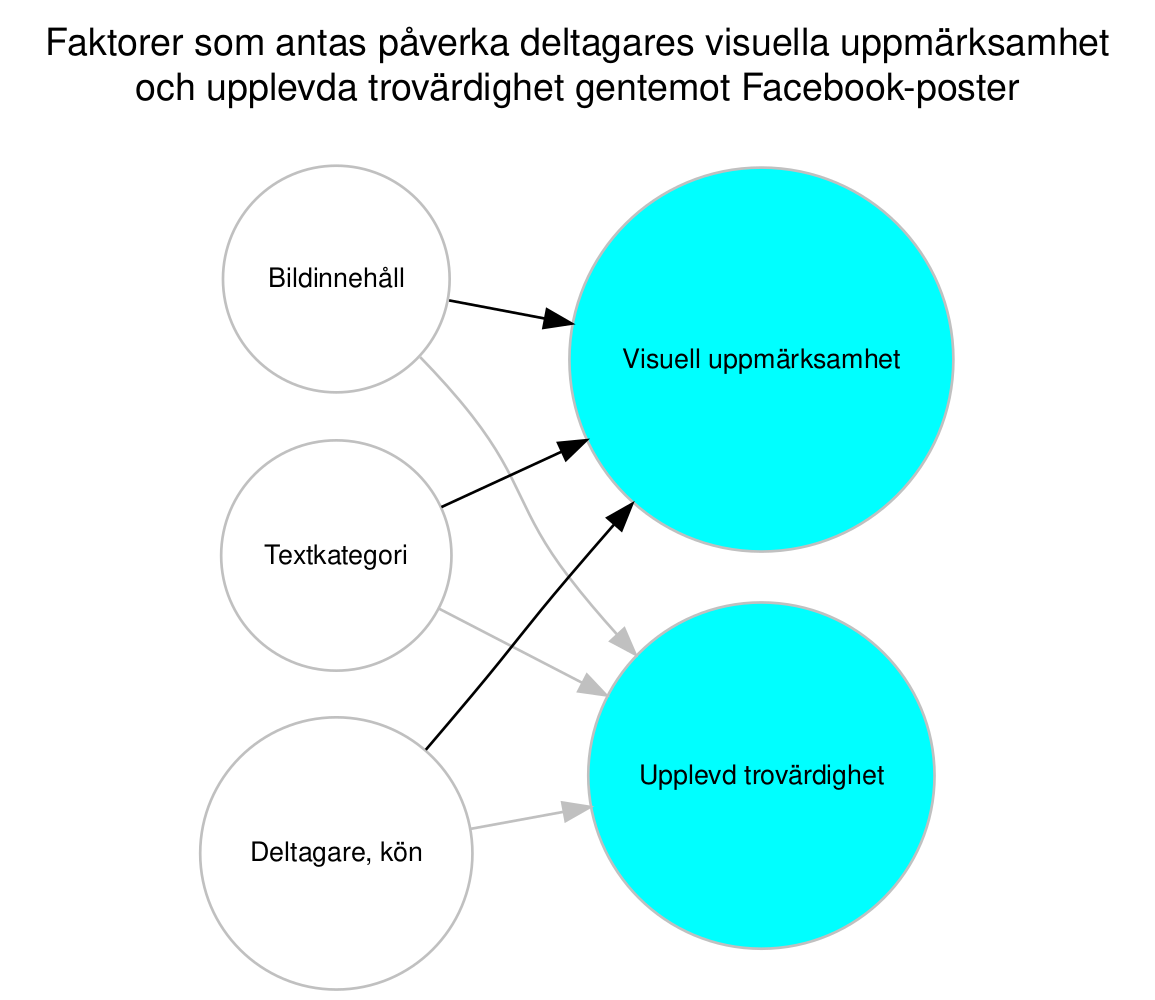
\includegraphics[width=0.8\linewidth]{../fig/graph} 

}

\caption{En teoretisk modell.}\label{fig:fig-02-06-3-0-01}
\end{figure}

\hypertarget{sub06.3.1}{%
\subsection{Planering av hypoteser}\label{sub06.3.1}}

Inom flera samhällsvetenskapliga ämnen använder man sig av ett ramverk som kallas "Null Hypothesis Significance Testing" (förkortat NHST) i samband med att man formulerar hypoteser inom ett experiment \citep{pernet2015null}. Detta ramverk säger i princip att varje hypotes ska uttrycka endast \emph{ett} förväntat samband mellan studiens variabler. Hypoteserna ska vara formulerade så att \emph{riktningen} på förväntade samband framgår. I vårt experiment förväntar vi oss till exempel att när bildinnehållet varieras från "neutral person" till "auktoritetsperson" så kommer visuell uppmärksamhet och upplevd trovärdighet att öka. Vidare ska hypoteserna formuleras så att de går att falsifiera. Nollhypotesen (H0) är att det inte finns någon statistiskt mätbar (signifikant) skillnad mellan villkoren. Om vi uppmäter en signifikant skillnad i våra beroende variabler mellan villkoren så förkastar vi nollhypotesen. Det är mycket svårare att bevisa att ingen skillnad finns mellan två villkor, än att bevisa att en skillnad uppmätts (det förra alternativet kräver andra statistiska metoder som ibland kallas för Bayesianska).

\hypertarget{sub06.3.2}{%
\subsection{Rapportering av hypoteser}\label{sub06.3.2}}

Rapportering av hypoteser brukar komma i slutet av introduktionen, före rapportering av metoder. Till skillnad från generella forskningsfrågor, försöker vi formulera dessa hypoteser som specifika antaganden gällande samband mellan variabler. Styrkan med en experimentell studie är att vi kan formulera hypoteserna som kausala orsakssamband. När vi först manipulerar en oberoende förklaringsvariabel såsom "bildinnehåll" antar vi alltså att denna variation sedan \emph{orsakar} skillnader i de beroende variabler vi använder för att mäta försöksdeltagarna beteende och attityder. Inom vissa delar av den psykologiska forskningen kallas denna relation för stimulus-respons. Vi kan prata om kausala samband så länge det är ett kontrollerat experiment. Svårare om det är ett naturligt experiment. Slutligen ska riktningen på förväntade samband framgå. När vi tagit hänsyn till dessa kan vi sedan formulera en hypotes per beroende variabel som ingår i vår undersökning:

\begin{itemize}
\item
  H1: Facebook-poster med bild på en auktoritetsperson kommer att orsaka mer visuell uppmärksamhet på posten jämfört med bilder som innehåller en neutral person.
\item
  H2: Facebook-poster med bild på en auktoritetsperson kommer att orsaka högre upplevd trovärdighet hos posten jämfört med bilder som innehåller en neutral person.
\end{itemize}

Enligt NHST-modellen föregås dessa hypoteser egentligen av en så kallad nollhypotes, under vilken vi antar att skillnader i bildinnehåll hos Facebook-poster \textbf{inte} kommer att orsaka några skillnader, varken vad gäller visuell uppmärksamhet eller upplevd trovärdighet. Nollhypotesen brukar inte explicit skrivas ut då den är underförstådd, men den hade kunnat formuleras ungefär som: "H0: Facebook-poster med bild på en auktoritetsperson kommer inte att ha någon effekt på visuell uppmärksamhet (eller upplevd trovärdighet) gentemot posten jämfört med bilder som innehåller en neutral person". Detta innebär att om vår studie inte finner stöd för t.ex. den första hypotesen (H1) så är den falsifierad, och vi kan därmed antar att resultaten stödjer motsvarande nollhypotes (H0).

The hypothetico-deductive model or method (step 1-4) this method can never absolutely verify (prove the truth of) 2. It can only falsify 2. This is what Einstein meant when he said, ``No amount of experimentation can ever prove me right; a single experiment can prove me wrong.'' \citep{einstein2002induction}

\hypertarget{chap07}{%
\chapter{Genomförande}\label{chap07}}

En av de viktigaste aspekterna av experimentell forskning handlar om att resultaten av ett specifikt experiment måste kunna reproduceras (eller replikeras) av en eller flera oberoende forskare. Om resultaten av ett experiment inte kan reproduceras, tyder detta på en godtycklighet i genomförandet, och man kan då med rätta ifrågasätta det vetenskapliga värdet av ett sådan experiment. Om resultaten av ett experiment inte kan upprepas så kan de heller inte jämföras med tidigare eller efterföljande studier inom samma forskningsområde. Det blir alltså omöjligt att bygga vidare på icke-reproducerbara resultat, och de resurser i form av tid och pengar man spenderat på att genomföra studien kan till största delen betraktas som bortkastade.

För att ge utomstående forskare (och i högsta grad, oss själva) en möjlighet att upprepa en forskningsstudie och förhoppningsvis erhålla liknande resultat, krävs en utförlig och standardiserad dokumentation av hur studien genomförts (Berger, 1977). Denna dokumentation kallas för studiens metod. Metoddelen av en forskningsrapport ska alltså kunna fungera som tillräckligt detaljerade instruktioner för att andra forskare ska kunna återskapa alla de viktigaste betingelserna under vilka vi erhöll våra egna forskningsresultat, t.ex. antal deltagare, mätinstrument, dataanalys, osv. Med anledning av detta har vi också standarder för hur vi bör rapportera forskning (t.ex. American Psychological Association, APA). Men experimentell metod handlar naturligtvis också om att praktiskt tillämpa vissa tillvägagångssätt som utvecklats för att vi ska kunna försäkra oss om att genomförande och resultat är så giltiga och tillförlitliga som möjligt (se diskussioner av validitet och reliabilitet).

I denna lärobok har vi försökt täcka in dessa två olika men näraliggande betydelser av begreppet experimentell metod: dels som en uppsättning praktiska tillvägagångssätt som bör användas för att i förväg \textbf{planera} och därefter genomföra en experimentell studie, och dels som ett systematiskt och standardiserat efterarbete för att \textbf{rapportera} genomförandet av en studie. Således är detta kapitel av läroboken disponerat på ett sätt som ger oss möjlighet att i ungefärlig turordning behandla de olika aspekter av experimentell metod som vi som forskare förväntas kunna redovisa när vi rapporterar våra resultat till en vetenskaplig tidskrift. Men inom varje metodaspekt kommer vi också att utförligt diskutera de olika experimentella tillvägagångssätt som är relevanta i samband med planering och genomförande av en forskningsstudie. - Ofta den första delen som skrivs när man rapporterar resultaten av en studie. Fördelaktigt att börja med en genomgång av hur studien faktiskt har genomförts.

I detta kapitel kommer vi arbeta efter en vanligt förekommande turordning som kan användas för att både genomföra och rapportera ett experiment. Förarbetet till studien är i detta skede redan avklarat, och genom att undersöka tidigare forskning har vi definierat en forskningsfråga, som genom operationalisering omsatts till falsifierbara hypoteser. Med detta som grund kan vi sedan inleda genomförandet i form av \emph{förstudier} som syftar till att säkerställa att studien som helhet håller en god kvalitet och är genomförbart. När vi känner oss säkra på att experimentet kommer fungera som tänkt kan vi börja rekrytera våra \emph{försöksdeltagare} enligt lämpliga urvalsprinciper. Deltagarna är naturligtvis avgörande när vi sedan ska använda ett \emph{mätinstrument} för att samla in data om studiens centrala utfallsvariabler, och vi utformar \emph{experimentella villkor} som vi i enlighet med hypoteserna förväntar oss kommer att ha en kausal effekt på dessa utfallsvariabler. Exakt hur varje deltagare kommer att genomgå kontrollvillkor och behandlingar definieras genom en \emph{experimentell design}. Genomförandet av experimentet kräver alltså mycket arbete innan vi kommit till den punkt där vi utvecklar en standardiserad \emph{procedur} genom vilken försökspersonerna deltar i experimentet. Den sista fasen av genomförandet består av en \emph{dataanalys} där vi bearbetar den rådata experimentet genererat och förbereder den för statistisk analys i studiens efterarbete.

\hypertarget{sec07.1}{%
\section{Förstudier och kvalitet}\label{sec07.1}}

Innan man genomför ett skarpt experiment, vilket ofta kräver mycket resurser i form av tid och arbete, är det klokt att genomföra experimentet i liten skala. På så vis kan vi som studenter eller forskarna i ett tidigt stadium fånga upp problem med experimentdesignen. Detta kallas för att vi genomför en förstudie eller ett pilottest. I sambad med planering och förberedelse av experimentet kommer vi också att diskutera det statistiska begreppet kraftanalys (från engelskans ``power analysis''). Men vi börjar med att i korthet behandla begreppen validitet och reliabilitet som ett slags ``kvalitetsmått'' på en vetenskaplig studie. För att experimentet som helhet ska hålla så hög kvalitet som möjligt är det viktigt att vi börjar förhålla oss till dessa begrepp redan tidigt i genomförandet av studien.

\hypertarget{sub07.1.1}{%
\subsection{Validitet och reliabilitet}\label{sub07.1.1}}

Intern validitet är i vilken utsträckning insamlade empiriska data stödjer våra antaganden om orsak och verkan. Det är en av de viktigaste egenskaperna hos vetenskapliga studier och är även ett viktigt begrepp i resonemang om evidens mer generellt. Intern validitet bestäms av hur väl en studie kan utesluta alternativa förklaringar till dess resultat (t.ex. systematiska fel eller ``bias''). Intern validitet handlar alltså om giltigheten av de slutsatser som dras \emph{inom} ramen för en viss studie. Detta står i kontrast till extern validitet, vilket handlar om giltigheten av att tillämpa slutsatserna från en vetenskaplig studie \emph{utanför} ramen för den studien. Extern validitet är alltså i vilken utsträckning resultaten av en studie kan generaliseras till andra situationer, människor, stimuli och tidpunkter. Eftersom generella slutsatser nästan alltid är ett primärt mål i vetenskaplig forskning, är extern validitet en viktig egenskap hos alla studier.

Förutom generaliserbarheten av resultaten av ett experiment, är det också viktigt att beakta kvaliteten på experimentets manipulationer, vilket är en del av området begreppsvaliditet (på engelska ``construct validity''). Ett annat exempel på begreppsvaliditet är hur väl ett test mäter ett abstrakt psykologiskt begrepp såsom aggressivitet eller viljestyrka. Låt oss ta ett lite mer utarbetat exempel: Sociologisk forskning har undersökt människans hjälpbeteende. Två forskare fokuserade mer specifikt på forskningsfrågan om hjälpbeteende blir mer utspritt ju fler personer som närvarar i en situation där hjälp behövs \citep{darley1968bystander}. Hypotesen var att deltagare i ett labb skulle bli mindre benägna att hjälpa till när de trodde att det fanns fler potentiella hjälpare förutom dem själva. Forskarna operationaliserade den oberoende variabeln för spridning av ansvar genom att öka antalet potentiella hjälpare. Vid en utvärdering av denna experimentdesign skulle vi säga att begreppsvaliditeten var hög eftersom experimentets manipulationer mycket tydligt motsvarar forskningsfrågan; det fanns en situation med hjälpbehov, samt ett sätt för deltagaren att hjälpa till, och genom att öka antalet andra deltagare som var närvarande skapades ett sätt att testa spridning hjälpbeteende.

Reliabilitet är en annan typ av kvalitetsmått som beskriver tillförlitligheten hos en mätning eller ett beteendevetenskapligt mätinstrument. Reliabilitet avser alltså ett måtts konsekvens. Inom samhällsvetenskapliga ämnen använder man framför allt tre typer av konsistens: över tid (på engelska ``test-retest reliability''), över testenheter (på engelska ``internal consistency'') och över olika forskare (på engelska ``inter-rater reliability''). När forskare mäter ett fenomen som antas vara konsekvent över tid, bör mätvärdena som erhålls också vara konsekventa över tid. Tillförlitlighet är i vilken utsträckning detta faktiskt är fallet. Till exempel anses intelligens i allmänhet vara konsekvent över tid. En person som är mycket intelligent idag kommer att vara mycket intelligent nästa vecka. Detta innebär att varje bra mått på intelligens bör ge ungefär samma poäng för denna individ nästa vecka som det gör idag. Uppenbarligen kan ett mått som ger mycket inkonsekventa poäng över tid inte vara ett särskilt bra mått på en konstruktion som är tänkt att vara konsekvent. Generellt tänker vi oss att reliabilitet kan beskrivas som:

\begin{itemize}
\tightlist
\item
  Observerat mätvärde = Sant mätvärde + Mätfel
\end{itemize}

En andra typ av tillförlitlighet är som sagt intern konsistens, vilket är graden av likvärdighet hos deltagares responser över olika enheter (på engelska ``items'') i ett test som består av flera enheter. I allmänhet antas alla enheter i ett sådant test återspegla samma underliggande fenomen, så människors mätvärden på dessa enheter bör vara korrelerade med varandra. Denna typ av reliabilitet mäter alltså om flera enheter som antas mäta samma generella fenomen ger liknande mätvärden. Till exempel, om en deltagare instämmer med påståendena ``Jag gillar att cykla'' och ``Jag har tyckt om att cykla tidigare'' och tar avstånd från påståendet ``Jag hatar cyklar'', skulle detta vara ett tecken på god intern konsistens hos detta specifika test.

\hypertarget{sub07.1.2}{%
\subsection{Power-analys}\label{sub07.1.2}}

När vi börjar omsätta vårt experiment till verklighet blir det naturligvis intressant att fråga oss själva hur många deltagare och/eller försök (trials) vi behöver ha med i experimentet för att ha en rimlig chans att få ett tillförlitligt resultat. Dessa funderingar har att göra med vad som på engelska kallas ``power analysis'', och vad vi på svenska ibland översätter till power-analys eller statistisk kraft \citep{ellis2010essential, sullivan2012using, cumming2013understanding}.

\begin{itemize}
\tightlist
\item
  \url{http://shinyapps.org/apps/PPV/}
\item
  \url{https://gallery.shinyapps.io/CLT_mean/}
\item
  \url{http://www.gpower.hhu.de/}
\end{itemize}

Den statistiska kraften (på engelska ``statistical power'') i en experimentdesign är sannolikheten att korrekt förkasta nollhypotesen, givet ett visst antal deltagare (urvalsstorlek) och den förväntade styrkan i sambandet mellan de variabler som är av intresse. För att ta ett konkret exempel, den statistiska styrkan i en studie med 50 deltagare och en förväntad korrelation på +0.3 (beräknat som Pearson's r) i populationen är 0.59. Detta innebär att sannolikheten att vi korrekt kan förkasta nollhypotesen är 59\% om det aktuella sambandet i befolkningen verkligen har en styrka på +0.3. Statistisk kraft är komplementär till sannolikheten att begå ett s.k. typ II-fel (att inte detektera en skillnad som stödjer hypotesen och därmed felaktigt anta nollhypotsen), så i föreliggande exempel är risken för ett sådant typ II-fel 1 -- 59 = 41\%.

Innan man genomför ett skarpt experiment är det således viktigt att vi gör en power-analys, eftersom detta hjälper oss att undvika typ II-fel när vi analyserar resultaten \citep{cohen1992power}. Mer specifikt bör vi försäkra oss om att vår forskningsdesign har en tillräcklig statistisk kraft innan vi börjar med genomförandet av experiment och datainsamling. Den vanligaste riktlinjen är att en statistisk power på 0.8 är tillräcklig, vilket innebär att vi får en 80\% chans att korrekt förkasta nollhypotesen vid den förväntade styrkan på sambandet mellan det variabler vi intresserar oss för.

\begin{longtable}[]{@{}lrr@{}}
\caption{\label{tab:tab-02-07-1-1-01}Antal deltagare som krävs för att uppnå statistisk kraft på 0.8 vid olika starka samband.}\tabularnewline
\toprule
Styrka.på.samband & Deltagare.t.test & Deltagare.Pearsons.r\tabularnewline
\midrule
\endfirsthead
\toprule
Styrka.på.samband & Deltagare.t.test & Deltagare.Pearsons.r\tabularnewline
\midrule
\endhead
Starkt (d=0.8, r=0.5) & 52 & 28\tabularnewline
Medel (d=0.5, r=0.3) & 128 & 84\tabularnewline
Svagt (d=0.2, r=0.1) & 788 & 782\tabularnewline
\bottomrule
\end{longtable}

Vad ska du göra om du upptäcker att din forskningsdesign inte har tillräcklig kraft? Föreställ dig till exempel att du genomför ett experiment mellan ämnen med 20 deltagare i vart och ett av två tillstånd och att du förväntar dig en medelskillnad (d = 0,50) i populationen. Den statistiska kraften i denna design är endast 0,34. Det vill säga, även om det finns en medelskillnad i populationen, så finns det bara ungefär en av tre chans att förkasta nollhypotesen och ungefär två av tre chans att begå ett typ II-fel. Med tanke på den tid och ansträngning som är involverad i att genomföra studien verkar detta förmodligen vara en oacceptabelt låg chans att förkasta nollhypotesen och en oacceptabelt hög chans att begå ett typ II-fel.

Med tanke på att statistisk power främst beror på relationsstyrka och urvalsstorlek, finns det i huvudsak två steg du kan vidta för att öka statistisk styrka: öka styrkan på sambandet eller öka urvalsstorleken. Att öka styrkan i relationen kan ibland åstadkommas genom att använda en starkare manipulation eller genom att mer noggrant kontrollera för demografiska variabler för att minska mängden brus i data (t.ex. genom att använda en inomgruppsdesign snarare än en mellangruppsdesign). Den vanliga strategin är dock att öka urvalsstorleken. För varje förväntad relationsstyrka kommer det alltid att finnas något prov som är tillräckligt stort för att uppnå tillräcklig kraft \citep{faul2007g, faul2009statistical}.

\hypertarget{sub07.1.3}{%
\subsection{Pilottest}\label{sub07.1.3}}

Det är ofta användbart att förstå utvecklingen av en experimentell studie som en iterativ process, där genomförandet successivt kan förbättras baserat på erfarnheter från tidigare genomföranden. Slutligen är det ofta en fördel att kunna rapportera ett pilottest eller en förstudie i samband med att sakkunniga forskare granskar och bedömer om det är lämpligt att publicera resultaten i en tidskrift.

I pilottestet har vi möjlighet att testa att alla delar i experimentet fungerar, både som isolerade moduler oberoende av varandra, och som sammanhängande steg i en övergripande experimentell procedur. Vi kan alltså testa att vi kan rekrytera rätt \emph{försöksdeltagare}, dvs. deltagare som uppfyller de demografiska egenskaper som vi eventuellt specificerat i forskningsfrågor och hypoteser. Vi kan även testa att deltagarna förstår hur de lämnar informetat samtycke till att vi bearbetar den data vi samlar in från dem, samt andra etiska aspekter av vår forskning.

En annan del av experimentet som är mycket viktigt att testa och utvärdera har att göra med de \emph{mätinstrument} vi ämnar använda för att samla in data. Här kan det handla om att undersöka att deltagarna förstår enkätfrågorna i ett survey-experiment på det sätt som vi tänker oss att de ska förstå dessa frågor, och på det sätt som vi själva förstår dessa frågor. Det är inte ovanligt att vi som forskare får en helt annan förförståelse av enkätfrågorna i och med att vi formulerat dem, jämfört med hur en oinsatt försöksdeltagarna förstår frågorna. Lika viktigt är det naturligtvis att deltagarna förstår de responsalternativ som hänger samman med enkätfrågorna.

En annan sorts \emph{mätinstrument} utgörs av olika typer av sensorisk apparatur som kan användas för att samla in någon form av fysiologiska responser, exempelvis en ögonrörelsemätare (på engelska även kallad en eye-tracker) som används för att uppmäta var på datorskärmen deltagarna riktar sin visuella uppmärksamhet. Pilottest används i detta sammanhang för att försäkra oss om att vårt handhavande av mätutrustningen är korrekt (t.ex. kalibrering, applicering av elektroder på deltagaren o.dyl.), samt att datainsamligen genererar mätdata med tillfredställande nogrannhet (engelska accuracy, jfr. precision). Oavsett vilken typ av mätinstrument vi använder i ett experiment, är det alltså viktigt att noga överväga på instrumentents validitet och reliabilitet. Här kan tidigare forskning vara till stor hjälp, t.ex. genom framtagning av testade och validerade survey-frågor osv.

Nästa steg i förstudien handlar om att testa de behandlingar eller \emph{experimentella villkor} som vi planerar att administrera till våra försöksdeltagare. Genom att variera dessa villkor förväntar vi oss ju att kunna uppmäta skillnader i deltagarnas responser. Här underlättar det ofta att använda sig av termerna kontrollvillkor och behandlingsvillkor (ett eller flera). Exakt hur deltagarna exponeras för dessa villkor är en del av vår \emph{experimentella design}. Detta kan lösas genom att deltagarna exponeras för olika visuella stimuli som visas på en datorskärm. Ibland kan det krävas lite grundläggande programmeringskunskaper för att implementera en experimentell design (triggers etc.).

När vi har mätinstrument och experimentdesign på plats, kan det vara läge att pilottesta \emph{proceduren} vi kommer att använda oss av i samband med att varje deltagare genomgår vårt experiment. Denna procedur kan handla om allt från hur vi hälsar och tar emot deltagaren, till hur vi applicerar eventuell mätutrustning, till vi kort intervjuar deltagaren efter att den deltagit. Det främsta syftet med detta förfarande är att vi vill försäkra oss om att proceduren blir så standardiserad som möjligt, dvs. att vi inte eliciterar missvisande data från några deltagare pga. att dessa behandlats annorlunda i något avseende. I förlängningen har detta att göra med experimentets reliabilitet.

Slutligen är det väl värt att samla in lite faktisk testdata, när vi väl har alla experimentets delar på plats. Genom att göra detta kan vi pilottesta den \emph{dataanalys} som kommer ligga till grund för experimentets resultat. I denna fas testa vi helt enkelt att vi kan omvandla våra mätningar och villkor till variabler.

\hypertarget{sec07.2}{%
\section{Försöksdeltagare}\label{sec07.2}}

De individer som deltar i en studie kallades tidigare kort och gott "subjekt" (på engelska "subjects"). På senare tid har man vänt sig emot detta något avhumaniserande språkbruk och istället antagit den generella termen "deltagare". Här använder vi ibland beteckningen ``försökspersoner'' eller "försöksdeltagare" för att ytterligare betona den experimentella forskningens användning av kontrasterande behandlingar, villkor eller "försök" för att studera dess effekter på deltagarna (på engelska kallas sådana upprepade försök oftast för "trials", vilket är ett viktigt begrepp inom området experimentdesign som diskuteras längre fram i detta kapitel). Vi skulle också kunna tänka oss ett experiment som inte involverar mänskliga försöksdeltagare överhuvudtaget. Tänk till exempel på en webbplats genomgår ("behandlas") med två olika typer av sökoptimeringsstrategier. Därefter undersöker vi hur båda sidor indexeras och listas bland Googles sökresultat. Den beroende responsvariabeln är rankning (page rank), lägre värden innebär mer positivt utfall. Testet kan upprepas i flera trials.

\hypertarget{sub07.2.1}{%
\subsection{Representativt urval}\label{sub07.2.1}}

Inom samhällsvetenskapliga forskningsområden är det vanligt att anta att deltagarna i en studie ska vara så representativa som möjligt i förhållande till en viss målpopulation. Tanken bakom detta är att man av praktiska skäl bara har möjlighet att inkludera en mindre grupp deltagare i en studie (t.ex. studenter på ett visst utbildningsprogram), och utifrån detta begränsade urval vill man sedan kunna generalisera undersökningens resultat till en större grupp människor (t.ex. alla universitetsstuderande i Sverige). Även om detta resonemang i grund och botten är rimligt, är det främst användbart inom större enkätstudier som syftar till att undersöka attityder, kunskaper och beteenden hos en avgränsad och väldefinierad population av individer. Ett annat vanligt exempel på enkätundersökning där deltagarnas representativitet är avgörande är politiska opinionsundersökningar. Utifrån drygt tusen deltagare vill man här kunna generalisera till hela Sveriges befolkning med relativt låg felmarginal.

\hypertarget{sub07.2.2}{%
\subsection{Demografiska egenskaper}\label{sub07.2.2}}

Inom experimentell forskning tenderar man att tänka lite annorlunda kring frågan om att erhålla ett representativt urval av försöksdeltagare till en studie. Det är framför allt två saker som föranleder detta. För det första är det vanligt att man använder sig av objektiva och mätbara observationer i ett experiment, till skillnad från subjektiva (självrapporterade) och kvalitativa observationer i en survey, vilket antas leda till lägre nivåer av brus i de mätningar som genomförs. För det andra är det vanligt att de experimentella effekter man studerar är så små och svåra att uppmäta, att alltför stora individuella skillnader hos deltagarna riskerar att generera så mycket brus att effekten av en behandling inte kan detekteras. Av dessa två skäl är det vanligt att man eftersträvar någorlunda homogena deltagargrupper när man syftar till att genomföra experimentella studier.

Att man delvis frångår principen om representativt urval inom experimentell metodik har alltså att göra med att man på olika sätt vill begränsa mängden slumpartade och systematiska mätfel, dvs brus. Detta är ett tänk som kommer från det naturvetenskapliga området signalbehandling (ref). Nackdelen med detta förfarande är naturligtvis att generaliserbarheten riskerar att minska, vilket oftast är en svaghet. Inom vissa utbildningssystem där deltagande i experimentella studier är obligatoriskt för studenter, har den experimentella forskningen kritiserats för att endast kunna generalisera till just den befolkningsgrupp som studenter vanligtvis tillhör, t.ex. 18-25-åringar med västerländskt ursprung och förhållandevis god socioekonomisk ställning \citep{henrich2010weirdest}. Referera till begreppen bakgrundsvariabler, kontrollvariabler.

En annan faktor som har stor betydelse i samband med urvalet av försöksdeltagare är naturligtvis om de forskningsfrågor man undersöker är kopplade till någon specifik befolkningsgrupp, t.ex. vad gäller ålder (barn eller äldre), språk (enspråkiga eller flerspråkiga) och kognition (funktionsnedsatta och normalbefolkning). Om så är fallet, blir det ju naturligt att rekrytera deltagare från just dessa grupper och därmed ge avkall på möjligheten att kunna generalisera sina resultat till en bredare population. I viss mån styrs alltså urvalet av försöksdeltagare av den tidigare forskning som vi med vårt experiment vill bygga vidare på och kontribuera till. Som en tumregel kan man dock säga att en experimentell studie brukar bygga på 20-100 deltagare, där åldersspannet inte är för stort, och könsfördelningen inte är för skev. Längre fram i detta kapitel kommer vi även att diskutera hur experimentdesign påverkar antalet deltagare som är lämpligt i en studie.

\hypertarget{sub07.2.3}{%
\subsection{Individuella egenskaper}\label{sub07.2.3}}

Vi har redan nämnt att inom samhällsvetenskapliga experiment är vi ofta intresserade av att undersökas hur människor påverkas av olika företeelser i deras omgivning. I den utsträckning vi är intresserade av hur människors mentala tillstånd påverkas (engelska ``cognitive states'') så försvåras detta av dessa tillstånd inte är direkt mätbara (t.e.x attityd brukar kallas en latent variabel), samt att människors individuella skillnader bidrar till stora variationer på en utfallsvariabel, vilket i sin tur kan bidra till höga nivåer av brus när vi försöker undersöka det statistiska sambandet mellan sådana latenta variabler. För att lösa detta kan vi behöva registrera variabler kring deltagarnas individuella skillnader, för att i ett senare skede eventuellt använda dem som kontrollvariabler.

\hypertarget{sub07.2.4}{%
\subsection{Etiska hänsynstaganden}\label{sub07.2.4}}

En internationell trend inom samhällsvetenskaplig forskning som gjort sig gällande under senare år är att stor vikt läggs vid forskarens etiska hänsyn gentemot dess försöksdeltagare. Exempelvis kan en journal kräva att ett experiment genomgått en etisk prövning innan det genomförs, i annat fall vill tidskriften inte publicera resultaten. Detta är naturligtvis i grunden en positiv utveckling, men det adderar ofta ett administrativt moment som behöver klaras av innan en studie kan sättas i verket. När en etisk kommitté utvärderar ett experiment är det framför allt två aspekter man tar hänsyn till: 1) att deltagaren inte ska lida några men i samband med genomförandet av undersökningen, och 2) att forskaren har en genomtänkt plan för hantering av forskningsdata som samlas in. Ett exempel på den första aspekten är analysera vilka villkor och manipulationer som förekommer, samt om mätutrustningen är invasiv eller inte. Exempel på det andra hänsynstagandet är att försöksdeltagares personliga integritet inte ska bli lidande (t.ex. känsliga personuppgifter), samt att forskningsdata ska hanteras på ett säkert sätt som även tillåter deltagaren att begära ut sina uppgifter i efterhand. Som regel är dessa hänsyn viktigare för anställda forskare; för studentprojekt brukar inte etisk prövning av studier vara nödvändigt.

\hypertarget{sub07.2.5}{%
\subsection{Planering av deltagare}\label{sub07.2.5}}

Här kommer några praktiska råd i samband med att man rekryterar försöksdeltagare till en experimentell studie. För det första, underskatta inte betydelsen av att få tillgång till motiverade personer som dels är omedvetna om syftet med experimentet, och dels är någorlunda representativa för den grupp av människor resultaten ska kunna generaliseras till. För det andra, underskatta inte den tid och möda som krävs för att lösa de logistiska aspekterna av att låta ett hundratal(?) individer genomgå de behandlingar som ett experiment består av under kontrollerade och likartade förutsättningar. Både bland forskare och studenter finns en föreställning om att planering av försöksdeltagare löser sig självt; så är dock inte fallet.

Redan på ett tidigt stadium är det viktigt att fastställa om det planerade experimentet är av en sådan art att det kräver etisk prövning, och i så fall måste studien godkännas av en etisk nämnd innan rekrytering av deltagare påbörjas. Etisk prövning blir ofta aktuellt om känsliga personuppgifter eller biometriska data samlas in, och om invasiv försöksutrustning som på något sätt kan förväntas påverka deltagaren används. I vårt exempel-experiment uppfylls inte dessa kriterier, eftersom tanken är att manipulera bildinnehåll i Facebook-poster, samt samla in data om deltagarnas blickbeteende och attityder.

Förutsatt att inga etiska hinder föreligger, kan rekryteringen av försöksdeltagare påbörjas genom att förslagsvis annonsera om studien och förse intresserade personer med kontaktuppgifter till försöksledaren (epost, telefonnummer, webblänk), samt möjlighet för presumtiva deltagare att ange dag och tid när de har möjlighet att delta. För att öka chanserna att folk ska anmäla sig till undersökningen kan det vara fördelaktigt att erbjuda någon form av ersättning, t.ex. en biobiljett eller en lunchkupong, dock underlättar det om ersättningsnivån inte överstiga ca 100 kr eftersom det då blir beskattningsbar inkomst.

I praktiken är det dock kanske viktigare att prata med tilltänkta försöksdeltagare och göra dem intresserade av forskningen och motiverade att avsätta tid för deltagande. Denna information måste då vägas mot att deltagarna ska vara omedvetna om syftet med det tilltänkta experimentet. Utgår vi återigen från vårt exempel-experiment, innebär detta att vi kan informera om att studien undersöker Facebook-användning, men att vi undanhåller hur vi manipulerat bildinnehållet i Facebookposterna (auktoritetspersoner gentemot neutrala personer). På forskningsjargong innebär detta att deltagarna avsiktligt hålls omedvetna eller "naiva" om studiens behandlingar, och att detta i sin tur minskar risken för påverkan eller "bias" i de observationer som samlas in.

Om vi förflyttar oss framåt i tiden till själva genomförandet av studien, så är det viktigt att betänka att varje försöksdeltagare ska ha rätt att ge informerat samtycke till studien innan den deltar (den engelska termen för detta är "informed consent"). Om deltagaren är yngre än 15 år krävs \textbf{dessutom} alla vårdnadshavares samtycke. Detta innebär att försöksledarna i förväg har en informationssida som beskriver forskarens respektive deltagarens rätt- och skyldigheter. Detta dokument ska undertecknas av deltagaren innan experimentet påbörjas. Forskaren har rätt att använda insamlade data för publikationer.

\hypertarget{sub07.2.6}{%
\subsection{Rapportering av deltagare}\label{sub07.2.6}}

När man väl genomfört studien och är i färd med att rapportera vilka personer som deltagit så krävs det vanligtvis betydligt mindre arbete än i planerings- och genomförandefasen. I artikeltexten läggs information om experimentets försöksdeltagare ofta som den första underrubriken till metodstycket, och det är också därför vi tar upp försöksdeltagare på just detta ställe i läroboken. Anledningen till att vi använder denna så kallade IMRD-disposition är det skapar en kronologisk struktur för både planering och rapportering av vetenskapliga studier, och för de som vill genomföra ett experiment kan det vara värdefullt att bekanta sig med denna konvention. - demografiska variabler, medelålder, range - representativt urval, population, bakgrundsvariabler, individuell variation - bortfall, missing cases

\hypertarget{sec07.3}{%
\section{Mätinstrument}\label{sec07.3}}

I en experimentell studie är det avgörande att införliva mätinstrument som på ett giltigt och tillförlitligt sätt kan uppmäta effekten av en behandling på en eller flera responsvariabler. En viktig anledning till att experiment och mätinstrument är nära förknippade, är att denna typ av positivistisk forskning syftar till att försöka säkerställa en faktisk skillnad mellan olika grupper av deltagare och olika typer av behandlingar, vilket till syvende och sist kräver analys med hjälp av statistiska metoder. Det räcker alltså inte med att forskaren rapporterar en subjektivt upplevd skillnad mellan försöksgrupper; denna skillnad måste bevisas!

I detta sammanhang bör mätinstrument uppfattas som ett relativt abstrakt begrepp; det kan röra sig om medicinsk eller fysiologisk mätutrustning, men i många samhällsvetenskapliga ämnen handlar mätinstrument ofta om enkätfrågor där svarsalternativen är utformade som Likert-skalor, exempelvis med skalsteg från 1-7. Med hjälp av ett sådant survey-instrument tänker man sig att det går att uppmäta försöksdeltagarnas attityder kring något ämne. Men man skulle också kunna tänka sig ett experiment inom marknadsföring som använder en binär mätvariabel. I detta fall skulle två deltagargrupper kanske titta på varsin version av en reklamfilm, och sedan svara "ja" eller "nej" på frågan om de var intresserade av att köpa den produkt som marknadsfördes i båda filmerna.

I det hypotetiska experiment som vi resonerar om i denna bok används två olika mätinstrument för att registrera olika typer av responser hos deltagarna i samband med att de tittar på Facebook-poster med bilder föreställande auktoritetspersoner respektive neutrala eller okända personer. I första steget används en ögonrörelsemätare för att mäta hur försöksdeltagarna visuella uppmärksamhet fördelar sig över Facebook-posten, och sedan används en 7-gradig Likert-skala för att mäta hur bildinnehållet påverkat deras attityder angående postens trovärdighet. De hypoteser som antagits för detta experiment är att auktoritetspersoner kommer att orsaka en ökning av visuell uppmärksamhet (dvs. hur länge deltagarna tittar på bilden), samt en ökning av upplevd trovärdighet hos posten (dvs. hur höga värden som väljs på Likert-skalan). En viktig skillnad mellan dessa två mätinstrument är att ögonrörelsemätning fångar ett objektivt beteende hos deltagaren, medan Likert-skalor registrerar mer subjektiva responser som rapporteras av deltagaren själv. Denna skillnad utvecklas lite mer i det följande (avsnitt \protect\hyperlink{sub07.3.2}{7.3.2}).

\hypertarget{sub07.3.1}{%
\subsection{Olika mätskalor}\label{sub07.3.1}}

Mätskala, eller ibland datanivå, är ett begrepp som används inom beskrivande statistik för att klassificera den variabel som mäts. Variabler som endast kan mätas enligt en nominalskala eller ordinalskala kallas med ett gemensamt namn kvalitativa variabler eller kategorivariabler och de som kan mätas enligt en intervallskala eller kvotskala kallas kvantitativa variabler. För kvantitativa variabler är det, förutom lägesmått som medelvärde och median, också möjligt att beräkna spridningsmått som standardavvikelse och varians (\url{https://sv.wikipedia.org/wiki/M\%C3\%A4tskala}). En viktig princip är att dessa skalor antas innehålla stegvis mer information, och man kan alltid ta bort information men den går inte att lägga till i efterhand (dvs vi kan omvandla en kvantitativ variabel till en kvalitativ, men inte omvänt). Det är alltså \emph{alltid bättre} att försöka använda en mätskala som innehåller så mycket information som möjligt.

\begin{longtable}[]{@{}lllll@{}}
\caption{\label{tab:tab-02-07-3-1-01}Mätskalor och information.}\tabularnewline
\toprule
Mätskala\_Information & Nominal. & Ordinal. & Intervall & Kvot\tabularnewline
\midrule
\endfirsthead
\toprule
Mätskala\_Information & Nominal. & Ordinal. & Intervall & Kvot\tabularnewline
\midrule
\endhead
Namn eller kategorier (binära, multiklass) & X & X & X & X\tabularnewline
Ordningsföljd eller rangordning & & X & X & X\tabularnewline
Mätningar med godtycklig nollpunkt & & & X & X\tabularnewline
Kontinuerliga mätningar med absolut nollpunkt & & & & X\tabularnewline
\bottomrule
\end{longtable}

\textbf{Nominalskala.} Det man mäter kan endast delas in i grupper utan inbördesordning. Exempel är kön, yrke och sjukdomstyp. Variabelns olika värden kan endast beskrivas med ord, exempelvis man/kvinna, läkare/sjuksköterska/städare/säljare. För variabler som mäts enligt en nominalskala är det möjligt att beräkna typvärde, men inte median eller aritmetiskt medelvärde.

\textbf{Ordinalskala.} Variabelns olika värden kan rangordnas, men det går inte att på något meningsfullt sätt ange skillnader eller avstånd mellan värdena. Exempel är utbildning som kan anta värdena grundskola/gymnasium/högskola/forskarutbildning. Det går att ordna värdena efter stigande utbildningsnivå, men man kan inte tilldela en viss utbildning något numeriskt värde. För en variabel mätt enligt denna skala är det möjligt att beräkna typvärde, median och percentiler, men inte aritmetiskt medelvärde. När vi i exempel-experimentet mäter deltagares attityd till Facebook-posters trovärdighet kallar vi detta ordinalskala, men vi behandlar den som en intervallskala av praktiska skäl.

\textbf{Intervallskala.} I detta fall kan det man mäter tilldelas ett numeriskt värde med ett konstant avstånd mellan de olika värdena. Ett exempel är temperatur mätt i grader Celsius. Det är här meningsfullt att ange skillnaden mellan två mätvärden. 20 grader Celsius är 10 grader varmare än 10 grader Celsius och 30 grader är ytterligare 10 grader varmare. Däremot är det inte riktigt att påstå att det en dag är dubbelt så varmt som föregående dag eftersom nollpunkten är godtycklig och det finns negativa temperaturvärden. För variabler mätta enligt denna skala är det möjligt att beräkna både typvärde, median och aritmetiskt medelvärde.

\textbf{Kvotskala.} Det som mäts kan beskrivas med ett kontinuerligt varierande numeriskt värde, och det finns ett entydigt sätt att definiera ett nollvärde. Därmed kan man jämföra storleken mellan de olika värdena. Exempel är kroppslängd mätt i centimeter. En person kan vara dubbelt så lång som en annan. Märk väl att det inte är i princip omöjligt att uppmäta negativa värden på en kvotskala. Exempelvis kan en persons samlade ekonomiska tillgångar anta ett negativt värde på en kvotskala om personens skulder överstiger dennes tillgångar. Endast för variabler som mäts enligt en kvotskala är det meningsfullt att multiplicera och dividera mätvärdena. När vi i exempel-experimentet mäter deltagares läsning av texten i Facebook-poster med hjälp av en ögonrörelsemätare, kan vi anse att detta utgör mätvärden på en kvotskala.

\hypertarget{sub07.3.2}{%
\subsection{Mätning av subjektiva responser}\label{sub07.3.2}}

En subjektiv respons innebär att det är helt upp till försöksdeltagaren att avgöra vilka mätdata man vill och kan lämna. Denna situation uppstår med nödvändighet i alla former av enkätfrågor, där själva frågekonstruktionen är öppen för deltagarens tolkning, och där deltagaren själv får bestämma vilket svarsalternativ den väljer att lämna som respons. Dessutom kan det uppstå systematiska felkällor (s.k. bias) beroende på hur forskaren samlar in svaren (t.ex. genom intervju eller skriftligt). Det är lätt att inse att ett sådant mätinstrument gör sig beroende av varje deltagares individuella förmåga och motivation att lämna giltiga svar, och att den mätdata som samlas in kommer att innehålla olika former av bruskällor som kan förvränga de sanna mätvärdena.

Även om enkätfrågor därmed kanske inte kan betraktas som en perfekt lösning, används de ändå flitigt inom den samhällsvetenskapliga forskningen, av det enkla skälet att detta mätinstrument ofta är det enda realistiska alternativet som står till buds om vi exempelvis avser att mäta deltagarnas attityder till ett fenomen, eller andra typer av mentala tillstånd. Man brukar säga att enkäter är lämpliga för att mäta deltagarnas \emph{beteenden} (t.ex. hur ofta de använder sociala medier på ett dygn), \emph{kunskaper} (t.ex. hur mycket de känner till om de algoritmer sociala medier använder för att presentera personligt innehåll till användaren), och \emph{attityder} (t.ex. om de har förtoende för hur sociala medier hanterar användarens personliga data).

För att hantera några av enkätens inneboende problem som mätinstrument har forskningen både förfinat själva frågedelen i enkäten, men också svarsalternativen. Detta kan åskådliggöras genom ett resonemang där vi antar att vi som forskare är intresserade av att mäta upplevd lycka bland en grupp människor. I detta exempel säger vi att det mentala tillståndet lycka är en latent variabel som vi inte kan mäta direkt, men som vi försöker komma åt genom att använda ett antal enkätfrågor som antas fånga olika aspekter av konceptet lycka. En fråga kan lyda ``hur lycklig är du i hemmet?'', en annan ``hur lycklig är du på jobbet?'', en tredje ``hur lycklig är du med dina vänner?'' osv. Förhoppningen är att flera likartade frågor sammantaget ska öka giltigheten (validiteten) i mätinstrumentet.

När det gäller svarsalternativ till dessa tänkta enkätfrågor om lycka, är det vanligt att använda så kallade likert-skalor, där deltagaren kan indikera ett värde mellan exempelvis 1 och 7, där lägre och högre värden betyder mindre respektive mer upplevd lycka, och mittenalternativet är neutralt. Genom att använda likartade skalor på flera enkätfrågor skapas ett någorlunda standardiserat format för svarsalternativen som deltagaren förhoppningsvis har lättare att ta ställning till. De numeriska värden som erhålls på varje individuell fråga kan sedan sammaställas till ett så kallat index genom att ta medelvärdet av deltagarens alla responser kring lycka. Detta antas öka tillförlitligheten eller reliabiliteten i mätinstrumentet. Men kom ihåg att denna typ av data är självrapporterad!

\hypertarget{sub07.3.3}{%
\subsection{Mätning av objektiva responser}\label{sub07.3.3}}

Objektiva responser är inte väsenskilda från subjektiva, och därför är det mer fruktbart att placera båda dessa responser på en skala av objektivitet, där enkätfrågor kan betraktas som mindre objektiva, och exempelvis fysiologiska responser anses mer objektiva. När det gäller enkätfrågor så betraktas ibland frågor som avser att undersöka respondentens beteenden som mer objektiva än frågor som frågor handlar om attityder (ref). Om vi flyttar fokus till fysiologiska mätmetoder så kan vi på samma sätt skilja mellan responser som är mer viljestyrda hos deltagaren (t.ex. var blicken riktas på en datorskärm), respektive mätdata som är mindre viljestyrd (t.ex. hur utvidgade pupillerna är). Det förra fallet handlar om mindre objektiva responser, det senare om mer objektiva. Subjektiva och objektiva responser är alltså ingen absolut distinktion.

\begin{longtable}[]{@{}llll@{}}
\caption{\label{tab:tab-02-07-3-3-01}Mätinstrument och objektivitet i mätdata.}\tabularnewline
\toprule
Minst.objektiv & Mindre.objektiv & Mer.objektiv & Mest.objektiv\tabularnewline
\midrule
\endfirsthead
\toprule
Minst.objektiv & Mindre.objektiv & Mer.objektiv & Mest.objektiv\tabularnewline
\midrule
\endhead
Attitydfrågor & Beteendefrågor & Voluntär respons & Involuntär respons\tabularnewline
\bottomrule
\end{longtable}

Låt oss utveckla resonemanget kring fysiologisk mätdata som potentiellt mer objektiva responser. Inom psykologisk, beteendevetenskaplig och medicinsk forskning skiljer man ofta på fysiska responser som är voluntära (viljestyrda) respektive involunära (icke-viljestyrda). Detta kan exemplifieras genom att betänka människans synsystem, där vi ibland viljemässigt styr vår visuella uppmärksamhet mot en specifik region i synfältet (endogenous attention), men ibland riktar blicken som en reflexmässig respons på att något oväntat plötsligt händer i vår omgivning (exogenous attention). Dessutom kan vi ibland rikta vår visuella uppmärksamhet mot något utan att direkt titta på det.

Detta resonemang säger oss att pupillens position \emph{ofta} utgör en relativt exakt indikator på var försöksdeltagaren riktar sin visuella uppmärksamhet, även om det finns undantag. Detta samband gör att vi kan använda ögonrörelsemätning som en mätmetod med hög grad av objektivitet och giltighet i situationer där vi vill förstå vilka yttre orsaker som påverkar visuell uppmärksamhet. I dessa situationer utgör visuell uppmärksamhet en latent variabel kopplad till människans kognition. Vi är ofta intresserade av att uttala om sådana kognitiva processer, men vi kan sällan direkt observera dem. Därför använder vi oss i detta fall av ögonrörelsemätning som en objektiv indikator på visuell uppmärksamhet.

För att ögonrörelsmätning ska fungera som en objektiv indikator för visuell uppmärksamhet krävs också att vi kan samla in data utan systematiska avvikelser (s.k. bias). Systematiska avvikelser kan inträffa om vi ställer in mätinstrumentet på ett felaktigt sätt, vilket exempelvis skulle kunna resultera i att alla uppmätta pupillpositioner förskjuts i någon rikting, vilket i sin tur betyder att vi relaterar deltagarens visuella uppmärksamhet till fel objekt på datorskärmen. För att undvika detta krävs kunskap om hur mätinstrumentet bör handhas, samt om hur vi kan kaliberera systemet för att ge tillförlitlig data oberoende av deltagarnas individuella fysiska egenskaper.

Andra exempel på fysiologiska och beteendevetenskapliga mätdata kan utgöras av observationer kopplade till deltagares användning av en webbläsare för att navigera en webbplats, t.ex. hur de använder en sökfunktion, hur länge de tittar på en video, eller vilka länkar de väljer att klicka på. Reaktionstidstest är också ganska vanligt. I dessa fall kan det vara underliggande kognitiva beslutprocesser som är av intresse för forskarna, eller så kan det vara klick-data i sig som är intressant. I många fall av fysiologisk datainsamling blir det viktigt att instruera deltagarna att genomföra någon form av uppgift i samband med att data spelas in. Detta för att minska variationen mellan individier (osystematiskt brus i data). Detta kan kräva mycket planering i studiens tillvägagångssätt. Instruktionen i vårt tänkta experiment skulle antagligen bli något i stil med ``försök bedömma trovärdigheten i följande fb-poster''. Detta för öka validitet och reliabilitet.

Här kan vi eventuellt använda en analogi från rättsväsendet, där man ibland skiljer mellan indicier (t.ex. vittnesuppgifter) och fysiskt bindande bevisning. Indicier handlar om bevismaterial som är mer subjektiva och därmed föremål för tolkning, vilket gör att det krävs mer sådan. Medicinska experiment där vi objektivt mäter 1) aktiv substans, 2) egenskaper hos deltagare, 3) antal viruspartiklar i blodet. Denna typ av direkta mätningar är inte alltid relevant inom samhällsvetenskaplig forskning.

\hypertarget{sub07.3.4}{%
\subsection{Beroende variabler}\label{sub07.3.4}}

I det tänkta experiment som ligger till grund för denna bok, använder vi oss huvudsakligen av två mätinstrument. Vi använder en så kallad ögonrörelsemätare (på engelska "eye-tracker") för att göra objektiva och kontinuerliga mätningar av hur läsarnas visuella uppmärksamhet fördelar sig över ytan på de Facebook-artiklar vi visar som stimuli på en datorskärm. Därefter använder vi en digital enkät som presenteras på samma datorskärmen \emph{efter} varje Facebook-post. Enkäten består av två-tre frågor om hur försöksdeltagaren upplever trovärdigheten i varje Facebook-post, och varje enkätfråga är kopplad till en likert-skala, där och olika aspekter av upplevd trovärdighet mäts på en skala mellan 1 och 7, och där högre värden används för att indikera högre trovärdighet.

Här gäller det att hålla i minnet att hälften av Facebook-posterna vi använder som stimuli i vår studie innehåller en bild på en okänd och därmed neutral person. Dessa stimuli används som experimentets kontrollvillkor. Den andra hälften av Facebookposterna kontrasterar mot detta villkor genom att innehålla bilder på auktoritetspersoner. Vi säger därmed att den senare hälften av posterna innehåller en behandling eller manipulation, vilket gör att dessa stimuli representerar det experimentets behandlingsvillkor. Vägledda av tidigare forskning inom denna medie- och kommunikationsforskning förväntar vi oss att stimuli som innehåller manipulationen ``bild på auktoritetsperson'' ska medföra en effekt på deltagarnas uppmätta responser. Eftersom vi tänker oss att responserna på ett systematiskt sätt \emph{beror} på en föregående behandling, kallar vi dessa responser för beroende variabler. Ibland kallas de också för utfallsvariabler eller responsvariabler.

Syftar generellt till att uppmäta och registrera en respons på ett stimuli eller en behandling, därför säger man ibland att syftet med mätinstrumenten är att på ett giltigt och tillförlitligt sätt mäta en responsvariabel. Ofta kontinuerlig eller binär (logistisk regression), men kan också vara multinomial eller kategorisk. Survey-frågor, svarsalternativ, likertskalor, attityder. "Beror" av en kronologiskt föregående orsak, dvs. behandling. På engelska kallas detta "dependent variable". Beroende variabler kallas ibland också mätvariabler eller utfallsvariabler. Jämför med oberoende variabler, förklaringsvariabler, experimentella villkor, behandlingar i nästa stycke av boken. På engelska "independent variable". Varje modell har \emph{en} beroende, flera oberoende variabler. Kausala samband har potentiellt större förklaringsvärde än associativa samband (korrelationer).

\hypertarget{sub07.3.5}{%
\subsection{Planering av mätinstrument}\label{sub07.3.5}}

När vi genomför ett experiment kräver detta nogrann planering av de mätinstrument vi avser att använda för att uppmäta deltagarnas responser i relation till kontrollvillkor respektive behandling. Ett typiskt experiment omfattar oftast mätning av \emph{en} responsvariabel, men i det tänkta experiment vi diskuterar i denna bok, mäter vi \emph{två} typer av responser med olika mätinstrument. Förutom att vi behöver planera hur vi ska använda varje enskilt mätinstrument, behöver vi alltså också planera för hur vi ska kombinera dessa mätningar. Den viktigaste principen här är att designa experimentet så att den ena mätningen inte alltför mycket påverkar den andra mätningen (systematiskt bias). Som exempel kan vi tänka oss en situation där vi först använder en survey för att mäta deltagarnas generella tilltro till innehåll på sociala medier, och sedan mäter deltagarnas visuella uppmärksamhet på en Facebook-post. I denna situation får vi anta den första mätningen (survey) till viss del influerar eller ``spiller över'' på den andra mätningen (blickbeteende). Beroende på vilken frågeställning experimentet är tänkt att svara på, kan detta vara mer eller mindre problematiskt. Generellt kan man säga att denna typ av priming-effekter bör minimeras, men ibland är de oundvikliga, och ibland är de till och med önskvärda (t.ex. i priming-experiment).

I denna bok använder vi ögonrörelsemätning som ett slags representant för flera typer av mätmetoder som kan kallas beteendevetenskapliga eller fysiologiska, dvs att de ämnar mäta npgon form av fysiska responser och/eller viljestyrt beteende. Förutom ögonrörelsemätning, är det ganska vanligt att man mäter hjärnaktivitet med hjälp av apparatur som kallas elektroencefalografi (EEG) eller magnetresonansavbildning (fMRI), eller reaktionstider uppmätt med hjälp av tagenttryckningar, eller datorinteraktion uppmätt med hjälp av datormus och tangentbord. I fallet med ögonrörelsemätning, liksom övriga nyss nämnda fysiologiska mätmetoder, är det vanligt att experimentledaren behöver en separat utbildning i hur systemet ska användas för att generera så korrekta data som möjligt. Det är dessutom vanligt att det krävs en etisk prövning av hur systemet appliceras på försöksdeltagaren samt hur experimentet exponerar deltagarna för sensoriska stimuli. Kontinuerliga mätningar ställer krav på användning av datorer och programvaror för att registrera mätdata, stimulus onset, trial duration, triggers.

Jämfört med fysiologiska mätmetoder är det relativt enkelt att administrera en enkät som mätinstrument. Dock kräver även detta mätinstrument att forskaren nogrant sätter sig in i metodlitteratur kring hur enkätfrågor och svarsalternativ bör utformas för ett generera så giltig och tillförlitlig mätdata som möjligt. När vi exempelvis försöker mäta en latent variabel som ``upplevd trovärdighet'' kan det vara viktigt att planera för flera olika enkätfrågor som var och en mäter olika aspekter av denna kognitiva process. Dessutom är det viktigt att planera utformningen av svarsalternativ i form av likert-skalor till respektive enkätfråga. Tillvägagångssätt, planering. Diskutera utifrån exempel-experiment med bildinnehåll hos Facebook-poster. Ögonrörelsemätning för visuell uppmärksamhet, Likert-skalor för attitydmätning. Giltighet och tillförlitlighet hos alla mätvariabler, beroende variabler som används i studien. Återkoppla till pilottest. use multiple indicators of trust in leif gw facebook posts..

\hypertarget{sec07.4}{%
\section{Experimentella villkor}\label{sec07.4}}

Ett typiskt experiment består ofta av ett kontrollvillkor och ett eller flera behandlingsvillkor. Ett kontrollvillkor refererar till ett slags naturligt normaltillstånd, som kännetecknas av att deltagaren \emph{inte} genomgår någon form av behandling, eller exponeras för någon form av manipulation. Experimentella villkor å andra sidan betyder att försöksdeltagaren genomgår just en sådan behandling (t.ex. genom att inta en verksam medicinsk substans) eller utsätts för en manipulation (t.ex. genom exponering för en viss nivå av belysning). I ett enkelt experiment förekommer endast dessa två tillstånd, vilket kan beskrivas med en s.k. oberoende variabel, där frånvaron av behandling (kontrollvillkor) exempelvis representeras av den numeriska symbolen ``0'', medan förekomsten av en behandling (behandlingsvillkor) representeras av symbolen ``1''. I termer av mätnivåer, skulle en sådan variabel kallas binär. I mer invecklade experiment kan det förekomma kombinationer av flera olika behandlingar (t.ex. intag av medicin \emph{och} exponering för belysning) som dessutom utdelas i flera olika \emph{nivåer} (t.ex. ``ingen dos'', ``låg dos'', och ``hög dos''). Mer om detta längre fram.

Genom att mäta försöksdeltagarnas responser med hjälp av någon relevant beroende variabel (t.ex. blodtryck) under både kontrollvillkor och experimentella villkor, undersöks därefter eventuella skillnader mellan dessa villkor. Hittar vi sådana skillnader kan vi tala om \emph{effekter} av behandling jämfört med normaltillståndet. På engelska kallas sådana villkor ofta för ``conditions'' eller ``treatments''. I detta sammanhang är det viktigt att betänka att kontrollvillkor och experimentella villkor (``conditions'') bör betraktas som abstrakta begrepp, vilka sedan behöver konkretiseras i form av faktiska, reella behandlingar (``treatments''), ofta med hjälp av teknisk utrustning och laboratoriemateriel, samt en standardiserad procedur för att utdela dessa behandlingar. Denna process, i vilken abstrakta villkor implementeras som någon form av konkreta behandlingar, kallas ibland för \emph{operationalisering} (se tidigare avsnitt 6.2). Inom ett experiment är det även vanligt att behandlingar upprepas ett visst antal gånger, vilket kallas för försök, eller på engelska ``trials'' (se experimentdesign nedan).

\hypertarget{sub07.4.1}{%
\subsection{Kontroll- och behandlingsvillkor}\label{sub07.4.1}}

Låt oss återvända till bokens tänka exempel-experiment för att utveckla och konkretisera resonemanget kring experimentella villkor. Som vi har sagt tidigare, kräver den enklaste formen av ett experiment en kontrast mellan att deltagarna genomgår en behandling eller att de inte gör det. Att \emph{inte} genomgå en behandling kallas för ett kontrollvillkor, och dessa deltagare sägs därmed tillhöra kontrollgruppen. I fallet med medicinsk forskning kan detta villkor tyckas ganska uppenbart: det kan bestå i att en grupp deltagare inte tilldels ett läkemedel (eller att de tilldelas ett verkningslöst sockerpiller). Men i samhällsvetenskapliga experiment kan det vara betydligt svårare att definiera vad som egentigen är ett kontrollvillkor.

I vårt Facebook-experiment exponeras deltagare för två olika typer av bildinnehåll -\/- antingen presenteras en Facebook-post med en bild på en auktoritetsperson, eller en bild på en neutral person. Vilket av dessa två bildvillkor utgör då kontrollvillkoret? Båda grupperna av försöksdeltagare exponeras ju för någon form av bild, och omvänt, ingen av grupperna får titta på Facebook-posten utan bild. För att resonera om kontrollvillkoret i detta exempel kan vi börja med att tänka oss samtliga bilder på personer som existerar på Facebook. Därefter låter vi en slumpmässigt utvald Facebook-användare titta på tio slumpmässigt utvalda bilder ur samlingen av alla bilder. Slutligen ställer vi oss frågan: kommer denna användare se fler bilder på okända, och i den meningen neutrala personer, eller kommer användaren att se fler bilder som han eller hon relaterar till som auktoritetspersoner? Statistiskt sett skulle vi antagligen säga att de flesta bilderna användaren ser troligen kommer föreställa okända och därmed neutrala personer, och därigenom kan vi resonera att Facebook-bilder med neutrala personer bör utgöra vårt kontrollvillkor. Mer generellt uttryckt är det vanligt att kontrollvillkoret får motsvara det typiska fallet, medan behandlingsvillkoret innehåller en ``otypisk'' manipulering av något slag.

Behandlingsvillkoret består därmed i att visa en Facebook-post med en bild föreställande en auktoritetsperson. För att ta ett konkret exempel kan vi anta att personen Leif G.W. Persson för många användare utgör en auktoritet i samband med Facebook-poster gällande kriminalitet. Att presentera en Facebook-post om kriminalitet tillsammans med en bild på Leif G.W. Persson skulle alltså utgöra behandlingsvillkoret i vårt experiment, medan att presentera samma Facebook-post med en neutral och okänd person skulle utgöra kontrollvillkoret. Det är mycket viktigt att betona att Facebook-posten (om kriminalitet) är samma i båda villkoren, medan bildinnehållet (auktoritetsperson respektive neutral person) varieras.

Detta innebär att så mycket som möjligt i Facebook-posten hålls konstant över båda villkoren, medan en enda aspekt varieras. Detta är helt centralt för experimentell metod, eftersom det innebär att om vi uppmäter skillnader i de beroende variablerna (visuell uppmärksamhet och upplevd trovärdighet) så kan dessa skillnader mer sannolikt härledas till själva bildvillkoren och inget annat. Denna härledning blir betydligt svårare eller kanske till och med omöjlig att göra om vi samtidig varierar andra egenskaper hos Facebook-posten, t.ex. antal gillningar och rubriktext. I en undersökning är alltså behandlingsvillkor och kontrollvillkor lika viktiga, och allt annat utom själva villkoren bör hållas konstant.

använder behandlingsvillkor i rubriken till detta stycke mest för att skapa en tydlig kontrast till kontrollvillkor i föregående avsnitt. Behandlingsvillkor benämns nämligen ofta som experimentella villkor, och fortsättningsvis kommer vi huvudsakligen använda denna beteckning.

\hypertarget{sub07.4.2}{%
\subsection{Oberoende variabler}\label{sub07.4.2}}

Oberoende variabler hänger konceptuellt samman med experimentella villkor, eller behandlingsvillkor, på så sätt att oberoende variabler används för att operationalisera experimentella villkor. Här påminner vi oss som hastigast om att operationalisering hittills definierats som att göra ett koncept mätbart. Vi kan nu utveckla och konkretisera denna definition genom att säga att en oberoende variabel registrerar varje gång en försöksdeltagare genomgår kontrollvillkoret eller behandlingsvillkoret inom en undersökning. Denna registrering görs i praktiken ofta med hjälp av ett datorprogram för hantering av tabelldata (registerdata) såsom Microsoft Excel, där första kolumnen kan tänkas innehålla alla deltagare i undersökningen (t.ex. deltagarnummer "1", "2", "3", osv), medan den andra kolumnen registrerar om respektive deltagare exponerats för kontrollvillkoret ("Kontroll") eller behandlingsvillkoret ("Behandling"). Med hjälp av denna uppställning kan alltså en enda oberoende variabel (kolumnen "Villkor" i figuren nedan) användas för att representera både kontrollvillkor och behandlingsvillkor. Slutligen används en kolumn för att registrera eller uppmäta den beroende variabeln i undersökningen (kolumnen "Utfall"), vilket behandlades i föregående kapitel.

\begin{longtable}[]{@{}rll@{}}
\caption{\label{tab:tab-02-07-4-2-01}Experimentella villkor och oberoende variabler.}\tabularnewline
\toprule
Deltagare. & Villkor. & Utfall\tabularnewline
\midrule
\endfirsthead
\toprule
Deltagare. & Villkor. & Utfall\tabularnewline
\midrule
\endhead
1 & Kontroll & Oförändrat\tabularnewline
2 & Behandling & Positivt\tabularnewline
3 & Kontroll & Oförändrat\tabularnewline
4 & Behandling & Oförändrat\tabularnewline
\bottomrule
\end{longtable}

I exempel-experimentet som beskrivs i denna bok, skulle kolumnen "Villkor" i figuren ovan kanske innehålla värdena "Neutral person" (för kontrollvillkoret) eller "Auktoritetsperson" (för behandlingsvillkoret), beroende på vilken typ av Facebook-post respektive deltagare exponerats för i undersökningen. I detta fall blir både kategoriska variabler. Skulle finnas två utfallsvariabler, nämligen visuell uppmärksamhet mätt i sekunder, samt upplevd trovärdighet mätt på en skala från 1-7. - stratifierat urval, på engelska ``randomized block design'', blocking variable: gender

Experimentella villkor är starkt kopplade till oberoende variabler. Inom den experimentella forskningen syftar begreppet på klargörandet av vilka mätvariabler som uppmäts i en undersökning (oftast en eller flera \emph{beroende variabler} kopplade till deltagarnas responser), samt vilka variabler som varieras eller manipuleras i undersökningen (oftast en eller flera \emph{oberoende variabler} kopplade till undersökningens behandlingar). En undersökning skulle till exempel kunna fokusera på effekten av olika typer av lärarledd feedback på studenters studieresultat (dock inte inlärningsförmåga). I denna situation representerar lärares feedback den oberoende variabeln, medan något mått på studenters inlärning kan representera den beroende variabeln. Förutom att klargöra dessa två kategorier av variabler, så bör den experimentella designen också specificera de olika värden eller nivåer som de oberoende variablerna kan anta. I exemplet med inlärning ovan kan man tänka sig att variabeln "lärares feedback" kan anta värden som varierar mellan "positiv", "negativ" eller "neutral" feedback. I detta fall skulle man säga att den oberoende variabeln feedback har tre olika nivåer eller "levels" på engelska (dessa nivåer kan vidare betraktas som mer kategoriska eller mer kontinuerliga till sin natur, se variabler kapitel xx). Här är det viktigt att tydliggöra att dessa nivåer på den oberoende variabeln är den operationaliserade versionen av de experimentella villkor vi diskuterade i kapitlet innan.

\hypertarget{sub07.4.3}{%
\subsection{Instruktionsvillkor}\label{sub07.4.3}}

En viss uppgift eller instruktion kan också fungera som ett experimentellt villkor. I sådana fall kontrasteras ofta denna uppgift mot ett kontrollvillkor där ingen uppgift eller instruktion ges (t.ex. fri interaktion). Vi kan alltså använda instruktioner för att ge olika uppgifter till två grupper av deltagare, medan resten av experimentet är identiskt för båda grupperna, och i så fall utgör själva uppgiften experimentets manipulation. Låt oss ta ett konkret exempel i form av en undersökning där varje deltagare får titta på ett antal bilder som visas en i taget på en datorskärm samtidigt som vi spelar in deltagarens blickbeteende. Hälften av deltagarna får instruktionen att titta fritt på bilderna (på engelska kallas detta ofta för "free-viewing"), medan den andra hälften får instruktionen att leta efter ett specifikt objekt i varje bild (på engelska kallas detta experimentella paradigm "visual search"). Genom denna variation i instruktioner har vi skapat ett experiment med mellangruppsdesign, innehållande ett kontrollvillkor (titta fritt), samt ett behandlingsvillkor (hitta objekt). Vi kan därefter undersöka om blickbeteende mellan dessa grupper systematiskt skiljer sig åt på det sätt vi antagit i våra hypoteser. (Se även kapitel om experimentdesign, samt kapitel om procedur.)

\hypertarget{sub07.4.4}{%
\subsection{Kontrollvariabler}\label{sub07.4.4}}

Vid det här laget har förhoppningsvis läsaren fått en någorlunda klar uppfattning om innebörden i begreppen \emph{kontrollvillkor} resp. \emph{behandlingsvillkor}, samt begreppen \emph{beroende variabel} resp. \emph{oberoende variabel}. Därför kommer vi här att introducera det nya begreppet \emph{kontrollvariabel} som kan komplicera bilden något, och som därför bäst förstås i kontrast till tidigare nämnda begrepp. Enkelt uttryckt beskriver kontrollvariabler sådana variabler som vi försöker mäta upp inom ett experiment för att dessa variabler inte ska konfundera de statistiska modeller som användes för att utvärdera och sammanställa experimentets resultat (jfr. engelskans ``confounds''). Vad betyder detta? Jo om vi inte håller koll på vissa variabler under experimentets genomförande så riskerar de att på mer eller mindre oförutsägbara sätt snedvrida resultaten, och detta vill vi naturligtvis undvika.

Låt oss ta ett konkret exempel på kontrollvariabler. Vi genomför ett experiment med syfte att undersöka hur två olika nivåer av rumsbelysning (normalt och svagt ljus) påverkar deltagarnas förmåga att läsa text på en datorskärm (exempelvis läshastighet och/eller läsförståelse). Vi rekryterar ett representativt urval av befolkningen som deltagare i studien och låter därefter två slumpmässigt utvalda grupper läsa på datorskärm under var sitt belysningsvillkor. Enligt tidigare forskning förväntar vi oss att gruppen som läste under svag rumsbelysning ska prestera något sämre vad gäller läshastighet jämfört med gruppen som läste under normal belysning. Men när vi sammanställer resultaten visar det sig till vår förvåning att båda grupperna har lika bra läsninghastighet.

Vad är det som har hänt här? När vi går tillbaka och undersöker våra experimentgrupper upptäcker vi kanske att det slumpmässiga urvalet resulterade i fler äldre personer i gruppen som läste under normal belysning, och fler yngre i gruppen som läste under svag belysning. Eftersom yngre personer generellt sett har bättre syn än äldre, resulterade den skeva ålderfördelningen mellan grupperna att läsprestationen var lika god under båda belysningsvillkor. Hade vi studerat tidigare forskning tillräckligt noga hade vi vetat att synsystemet har inte en konstant funktion över alla åldrar, utan försämras ganska kontinuerligt från medelåldern och framåt. För att isolera effekten av synförmåga från effekten av rumsbelysning hade vi i detta fall alltså behövt mäta varje deltagares \emph{ålder} som en kontrollvariabel, och ta med denna i den statistiska sammanställningen av studiens resultat.

Vad vi stött på här ett typ 2 fel, falskt negativt resultat (``type 2 error''). Det är värt att notera att om åldersfördelningen varit skev åt andra hållet, dvs att fler äldre personer råkade befinna sig i villkoret med svag rumsbelysning, så hade resultaten indikerat en överdrivet stor skillnad i läsförmåga mellan grupperna. I detta fall hade vi pratat om ett typ 1 fel, vilket kan vara svårare att upptäcka eftersom resultaten går i den riktning vi förväntar oss. Vi tycker oss i någon mening få bättre och tydligare resutat, trots att vi i sjäva verket fått ett missvisande resultat. Sammanfattningsvis handlar kontrollvariabler egentligen om att vi under ideala förhållanden kanske skulle vilja mäta allt, men vi måste begränsa oss av praktiska skäl, och mäta (och därigenom kontrollera) de viktigaste felkällorna i en undersökning.

\hypertarget{sub07.4.5}{%
\subsection{Utrustning och materiel}\label{sub07.4.5}}

När vi genomför ett experiment så brukar det förr eller senare bli aktuellt att fundera på den kanske mest fysiska nivån i undersökningen. Denna materiella nivå har att göra med den tekniska utrustning vi använder för att presentera stimuli för deltagarna samt för att uppmäta och registrera deras responser. Det kan tyckas sekundärt att beskriva denna nivå i detalj, men i själva verket är just detta viktigt ur metodologisk synvinkel, eftersom det har att göra med andra forskares möjlighet att upprepa resultaten av experimentet. Om vi inte utförligt beskriver vilken utrustning och materiel vi använt i studien minskar möjligheterna att replikera studiens resultat, vilket i sin tur minskar studiens vetenskapliga värde.

I detta avsnitt kommer vi fokusera på utrustning och materiel i samband med presentation av stimuli och experimentella villkor, men samma typ av diskussion är naturligtvis också relevant i relation till den mätutrustning vi använder för att registrera responser. I detta senare fall används på engelska ofta termen ``apparatus'', i kontrast till ``materials'', som mer typiskt används för att beskriva den materiel som används för att presentera stimuli (jfr. avsnitt \protect\hyperlink{sec07.3}{7.3} ovan). Innan vi sätter igång med detta är det här läge att vi drar oss till minnes att ett experiment omvandlar abstrakta villkor till konkreta behandlingar genom en process som vi kallar för operationalisering.

I följande beskrivning kommer vi gå igenom några olika sätt vi som forskare kan använda oss av för att distribuera behandlingar till deltagarna i en undersökning. Låt oss därvid börja med vårt invanda exempel-experiment. I detta fall står vi inför utmaningen att presentera ett antal Facebook-poster på en datorskärm, där varje post kan ingå i ett av två villkor (post-bild med neutral person i kontrollvillkoret, respektive auktoritetsperson i behandlingsvillkoret). Den utrusting och materiel som krävs för att realisera detta är i grunden: 1) en metod för att skapa Facebook-poster som ser autentiska ut och som för varje post låter oss variera den tillhörande bilden i enlighet med våra två experimentella villkor; 2) en metod för att generera ett digitalt formulär med en 7-gradig likert-skala där deltagarna kan ange den nivå av förtroende varje Facebook-post ger upphov till; 3) en metod för att presentera dessa Facebook-poster på en datorskärm för deltagarna.

\hypertarget{sec07.5}{%
\section{Experimentell design}\label{sec07.5}}

Design är ett svårdefinierat begrepp, vars innebörd handlar om att på ett överskådligt sätt sammanfatta strukturen och planen hos en vetenskaplig undersökning (på svenska används ibland ``upplägg'' eller ``planering'' som synonymer till experimentdesign). Begreppet experimentell design har två centrala aspekter: den första är kopplad till att beskriva och specificera de beroende och oberoende variablerna som ingår en undersökning, medan den andra centrala aspekten är kopplad till att beskriva hur deltagarna i en undersökning exponeras för de experimentella villkor som omfattas av de oberoende variablerna, dvs hur behandlingar (eller ``trials'' eller försöksomgångar) är distribuerade inom en experimentell studie. I det följande ska vi börja med att diskutera experimentell design i relation till oberoende variabler, vilka vi även refererar till som behandlingsvariabler i denna bok.

För att få en bättre förståelse av begreppet experimentdesign börjar vi med ett exempel från den medicinska forskningen. En epidemiologisk forskare bestämmer sig för att testa ett nytt vaccin som den tagit fram. För att undersöka detta bestämmer sig forskaren för att rekrytera försöksdeltagare som sedan delas in i två grupper, varav den ena gruppen får en overksam spruta med saltvattenlösning, och den andra gruppen får en spruta med det nya vaccinet. Vi säger därför att detta experiment har en \emph{mellangruppsdesign}, eftersom effekten av den oberoende variabeln (vatten vs.~vaccin) mäts och jämförs mellan två likvärdiga grupper av deltagare. Som tumregel kan man säga att en enklare experimentdesign är ofta att föredra framför en mer komplicerad design. Orsaken till detta är att en enkel design ofta genererar tydligare resultat som i efterhand är enklare att tolka. Enklare experimentella designer består ofta bara av en enda oberoende variabel som kan vara antingen numerisk eller kategorisk (i den engelska metodlitteraturen omnämns dessa ibland som ``quantitative'' respektive ``qualitative variables'').

Även om enkla experimentdesigner är idealet så finns det flera situationer där exempelvis en mellangruppsdesign inte riktigt räcker till. En sådan situation kan inträffa om den uppmätta effekten av en behandling på en viss utfallsvariabel är relativt liten jämfört med kontrollvillkoret. I sådana situationer riskerar alltså en eventuell effekt av behandlingen att drunkna i bakgrundsbruset från andra orsaksfaktorer. Ett konkret exempel på detta är undersökningar som mäter deltagarnas hjärnaktivitet (t.ex. genom elektroencefalografi eller EEG). En annan situation där en enkel mellangruppsdesign kan vara otillräckligt är om det naturligt förekommer stora individuella skillnader mellan deltagarna inom respektive försöksgrupp med avseende på utfallsvariabeln. Gemensamt för båda dessa problematiska situationer är alltså att den förväntade effekten av behandlingen är liten i relation till andra omgivande bruskällor (i överförd bemärkelse används ibland det engelska uttrycket ``low signal-to-noise ratio''), och att det därför föreligger en risk för typ I- och typ II-fel (s.k. ``false positives'' respektive ``false negatives'').

Just detta är ofta fallet i samhällsvetenskapliga undersökningar, där det är vanligt att kvantitativa data samlas in genom självrapporterade enkätsvar som ytterst är beroende av varje deltagares vilja och förmåga att svara uppriktigt, vilket kan skapa stor individuell variation. Här kan det alltså vara önskvärt att använda mer robusta experimentdesigner som kan hantera brusiga datainsamlingar innehållande flera potentiella felkällor. En lösning på detta problem är så kallad \emph{inomgruppsdesign}, vilket vi kommer diskutera längre fram i detta kapitel. Den tydligaste skillnaden gentemot mellangruppsdesign är dock att denna typ av experiment exponerar varje deltagare för både kontrollvillkor och behandlingsvillkor, samt att denna exponering kan upprepas flera gånger för varje deltagare. Av naturliga skäl är detta experimentella upplägg många gånger svårt eller omöjligt att genomföra inom den medicinska forskningen, eftersom försöksdeltagare inte både kan ges en placebotablett \emph{och} en verksam medicin vid samma tillfälle.

\hypertarget{sub07.5.1}{%
\subsection{Instruktioner och uppgifter}\label{sub07.5.1}}

Många samhällsvetenskapliga experiment brukar börja med en instruktion som ges till varje deltagare för att förklara vad som kommer hända, vilken uppgift som ska lösas, samt vad vi som forskare mäter hos deltagaren (dock nämner vi inte vad som har manipulerats i experimentets, eftersom deltagaren bör hållas omedveten om detta till efter att den är klar med undersökningen). Dessa instruktioner är i sig en viktig aspekt av experimentet, eftersom forskaren därigenom försöker uppnå en \emph{standardiserad} situation, där alla deltagare uppfattar experimentet på samma sätt, för att på så sätt öka validiteten och reliabiliteten hos insamlade data.

Men vi skulle också kunna använda instruktioner för att ge olika uppgifter till två grupper av deltagare, medan resten av experimentet är identiskt för båda grupperna, och i så fall utgör själva uppgiften experimentets manipulation. Låt oss ta ett konkret exempel i form av en undersökning där varje deltagare får titta på ett antal bilder som visas en i taget på en datorskärm samtidigt som vi spelar in deltagarens blickbeteende. Hälften av deltagarna får instruktionen att titta fritt på bilderna (på engelska kallas detta ofta för ``free-viewing''), medan den andra hälften får instruktionen att leta efter ett specifikt objekt i varje bild (på engelska ``visual search''). Genom denna variation i instruktioner har vi skapat ett experiment med mellangruppsdesign, innehållande ett kontrollvillkor (titta fritt), samt ett behandlingsvillkor (hitta objekt). Vi kan därefter undersöka om blickbeteende mellan dessa grupper systematiskt skiljer sig åt på det sätt vi antagit i våra hypoteser. I detta scenario är det viktigt att allt utom instuktionerna, dvs. de visuella stimuli visas för deltagarna, hålls konstant. Om både uppgift och stimuli varieras samtidigt uppstår risken att eventuella effekter inte kan härledas till endast en orsak.

Exemplet ovan handlar om en specifik användning av instruktioner för att generera ett experimentellt villkor. Mer generellt kan man säga att det ofta är fördelaktigt att ge deltagare någon form av uppgift i samband med ett experiment, eftersom man därigenom minskar variationen i hur deltagare interagerar med experimentets villkor. Mindre variation gör i sin tur att vi får större möjligheter att upptäcka statistiska skillnader mellan villkoren med avseende på någon utfallsvariabel. En uppgift av något slag gör deltagarna mer fokuserade. Dessutom innebär en uppgiftsstyrd eller målorienterad experimentdesign (engelska ``task-oriented'' eller ``goal-directed'') att vi som forskare får möjlighet att mäta uppgiftsprestation (engelska ``task performance''), vilket ofta är en mycket användbar utfallsvariabel.

\hypertarget{sub07.5.2}{%
\subsection{Randomisering och balansering}\label{sub07.5.2}}

Vi har hittills diskuterat de individer som deltar i experiment (\protect\hyperlink{sec07.2}{7.2 Försöksdeltagare}), de beroende variabler experimentet uppmäter hos deltagarna (\protect\hyperlink{sec07.3}{7.3 Mätinstrument}), samt de behandlingar som dessa individer genomgår (\protect\hyperlink{sec07.4}{7.4 Experimentella villkor}). När vi nu fortsätter med att diskutera experimentdesign (7.5), är förmodligen en av de viktigaste aspekterna begreppet ``randomisering'' \citep{fisher1936design}. Randomisering är så centralt att det ibland tas för givet inom den experimentella forskningen. Dock kan detta utgöra ett av de mer krävande momenten för studenter och forskare vad gäller att praktiskt designa ett experiment, eftersom randomisering ofta kräver grundläggande kunskaper i programmering för att genomföras. Bristfällig randomisering i experimentdesignen är ofta något som skapar problem när man analyserar effekten av experimentella villkor på en eller flera utfallsvariabler, och försöker dra slutsatser om statistiskt säkerställda effekter.

Randomisering (på engelska ``random assignment'') innebär i grund och botten att experimentledaren låter slumpen avgöra vilket experimentellt villkor (eller behandling) varje deltagare genomgår. I det enklaste fallet, där experimentet endast består av ett kontrollvillkor samt ett behandlingsvillkor, kan vi tänka oss att experimentledare låter varje deltagare singla slant, och beroende på utfallet tilldelar deltagaren ett av de två villkoren. Med tillräckligt många deltagare förutsäger slumpens lagar att fördelningen mellan två experimentella villkor kommer bli ungefär 50\% (krona eller klave), dvs. att hälften av deltagarna exponeras för kontrollvillkoret, och den andra hälften genomgår behandlingsvillkoret. Det viktigaste syftet med randomisering är dock att försäkra oss om att experimentledaren inte kan påverka experimentets genomförande, och att varje deltagare tilldelas ett villkor på ett sätt som är oberoende av vilket villkor alla andra deltagare tilldelas.

Dessutom kan randomiseringen användas för att hålla försöksdeltagaren i ovisshet om vilket behandlingsvillkor den exponerats för. Denna experimentdesign är vanlig i medicinska studier, och kallas då för en blind-studie (på engelska ``blinded experiment''), dvs. varje försöksdeltagare hålls omedveten om den får ett sockerpiller (kontrollvillkor) eller en verksam substans (behandlingsvillkor). Tanken med denna design är att reducera effekten av deltagarens förväntningar, den så kallade placebo-effekten, för att därigenom erhålla mer tillförlitliga resultat. Inom den medicinska forskningen är det också vanligt att gå ett steg längre, och därigenom även hålla försöksledaren omedveten om vilken behandling en viss deltagare tilldelas. I sådana fall talar man om en dubbel blind-studie (på engelska ``double-blind study''). Tanken med att hålla försöksdeltagaren omedveten om vilket experimentellt villkor den exponeras för, är besläktad med tanken att hålla deltagaren omedveten eller ``naiv'' om syftet med experimentet, dvs. vilka mätvariabler och behandlingsvariabler som används inom experimentet. Gemensamt för dessa designprinciper är syftet att reducera bias och öka tillförlitligheten hos studien.

Återgår vi till att diskutera randomisering mer specifikt, så kan vi konstatera att denna designprincip är ganska enkel och intuitiv så länge en studie bara kontrasterar två villkor, och där varje deltagare endast exponeras för ett av dessa villkor en gång. Denna så kallade mellangruppsdesign (vilken vi diskuterar mer utförligt i nästa avsnitt) fungerar ofta bra för enkla studier, men inom samhällsvetenskap och humanvetenskap kan det ibland krävas något mer avancerade experimentdesigner, vilket i sin tur kräver andra former av randomisering. Detta kan exempelvis inträffa om experimentet innefattar ett kontrollvillkor och \emph{två eller flera} behandlingsvillkor, eller om varje deltagare genomgår flera villkor, eller om experimentet innehåller någon kombination av dessa situationer. Betänk experimentdesignen som visas i tabellen nedan, där varje deltagare genomgår kontrollvillkoret samt två olika behandlingsvillkor.

\begin{longtable}[]{@{}llll@{}}
\caption{\label{tab:tab-02-07-5-2-01}Randomisering och balansering.}\tabularnewline
\toprule
Deltagare & Försöksomgång\_1 & Försöksomgång\_2 & Försöksomgång\_3\tabularnewline
\midrule
\endfirsthead
\toprule
Deltagare & Försöksomgång\_1 & Försöksomgång\_2 & Försöksomgång\_3\tabularnewline
\midrule
\endhead
Deltagare 1 =\textgreater{} & Kontroll & Behandling A & Behandling B\tabularnewline
Deltagare 2 =\textgreater{} & Behandling B & Kontroll & Behandling A\tabularnewline
Deltagare 3 =\textgreater{} & Behandling A & Behandling B & Kontroll\tabularnewline
Deltagare 4 =\textgreater{} & Kontroll & Behandling B & Behandling A\tabularnewline
Deltagare 5 =\textgreater{} & Behandling A & Kontroll & Behandling B\tabularnewline
Deltagare 6 =\textgreater{} & Behandling B & Behandling A & Kontroll\tabularnewline
Deltagare n =\textgreater{} & \ldots{} & \ldots{} & \ldots{}\tabularnewline
\bottomrule
\end{longtable}

I denna situation skulle vi som forskare kunna välja att låta varje deltagare först genomgå villkoret Kontroll, följt av Behandling A och Behandling B. Denna design vore kanske den enklaste att implementera, men den kan vara problematisk på andra sätt. För att konkretisera denna situation kan vi tänka oss ett experiment där varje deltagare får betrakta tre ansiktsbilder i följd. Den första bilden visar ett ansikte med neutralt ansiktsuttryck (Kontroll), medan det andra ansiktet visar ett sorgset minspel (Behandling A), och det tredje ansiktet visar en glad min (Behandling B). För varje ansikte försöksdeltagaren får betrakta, instrueras den att ange på en skala hur glad eller ledsen personen på bilden är. Skalan går från mycket ledsen (-10) till mycket glad (+10).

Problemet med denna experimentdesign, där villkoren inte randomiseras, inträffar om vi tänker oss att varje villkor i någon grad influerar nästkommande villkor (jfr. begreppet ``priming''). Detta skulle kunna inträffa om deltagarna, efter att ha betraktat det neutrala ansiktsuttrycket, upplever att det ledsna ansiktet är något mindre ledset än om det ledsna ansiktet hade betraktats först. På samma sätt skulle deltagarna kunna uppleva att det glada ansiktet är något mindre glatt efter att de betraktat det ledsna ansiktet. Denna typ av systematiska ordningseffekter (på engelska ``order effects'') är svåra att undvika helt, men med hjälp av randomisering kan vi åtminstone försöka minimera dem.

I ansiktsstudien ovan skulle vi kunna lösa randomiseringen på åtminstone två olika sätt. Det första sättet vore att ge varje bild 1/3 chans att presenteras som första, andra och tredje villkor. Detta kallas för randomisering utan ersättning (``randomization without replacement''). Det andra sättet vore att göra en lista med alla de sex möjliga ordningsföljder i vilka man kan presentera tre villkor, och sedan presentera villkoren enligt dessa ordningsföljder för de sex första deltagarna. Därefter upprepas ordningsföljderna för nästa sex deltagare. Denna metod kallas för ``latin square'', och innebär idealiskt att vi skulle behöva ett totalt antal deltagare i studien som är en multipel av sex (dvs. 12, 18, 24, osv.) för att designen ska vara helt balanserad. Randomisering är alltså viktigt om man kan misstänka att experimentella villkor skapar ordningseffekter, vilket som regel antas vara fallet i humanvetenskapliga och samhällsvetenskapliga studier. Att kontrollera för ordningseffekter genom randomisering är ofta mest kritiskt i studier med inomgruppsdesign och upprepade villkor, vilket kommer förklaras lite längre fram.

\hypertarget{sub07.5.3}{%
\subsection{Mellangruppsdesign}\label{sub07.5.3}}

Den enklaste formen av experimentell design (och därmed ofta den tydligaste) kan antagligen härledas från den medicinska forskningen. I denna experimentdesign ingår två stycken grupper av försöksdeltagare som i möjligaste mån är jämförbara (eller ``matchade'') vad gäller ett antal olika demografiska variabler, såsom ålder, kön och hälsotillstånd mm. Varje deltagargrupp blir sedan slumpmässigt tilldelad en behandling (t.ex. en ny blodtryckssänkande medicin som utvärderas) eller ingen behandling (t.ex. ett sockerpiller som antas vara fysiologiskt verkningslöst). Efter att varje försöksdeltagare genomgått en av dessa två behandlingar (eller experimentella villkor) undersöker experimentledaren effekten av respektive behandling genom att uppmäta värdet på en utfallsvariabel kopplad till alla deltagare i båda grupper (t.ex. blodtryck). Om den medicinska behandlingen haft en effekt jämfört med sockerpiller bör man finna en tydlig kontrast mellan deltagargrupperna (t.ex. lägre genomsnittligt blodtryck).

En något mer samhällsvetenskaplig tillämpning av mellangruppsdesign skulle kunna vara ett så kallat AB-test. Denna typ av experiment används relativt ofta inom kommunikationsvetenskap och marknadsföring, och i detta sammanhang kan syftet vara att ta reda på vilken typ av annonsdesign som ger bäst effekt på konsumenter. När det talas om AB-test så brukar det vara underförstått att en annons utformas i två varianter (A och B), där kommunikatören försöker manipulera en enda aspekt mellan varianterna. Exempelvis kan vi tänka oss att annonsen innehåller bild och text, och att experimentet undersöker effekten av att ha samma bild i annonserna, men olika formulering av texten, eller vice versa. Varje annonsvariant visas sedan för en grupp av deltagare, och efter varje individuell annonsexponering undersöks effekten på t.ex. uppmärksamhet, minne eller köpintresse hos deltagare i båda grupper. Utmaningen i denna typ av experiment ligger ofta i att hitta relevant tidigare forskning och att bara variera en enda aspekt mellan båda annonsvarianter. Eftersom det kan vara svårt att avgöra vilken variant som är kontrollvillkoret talar man i dessa fall bara om två olika behandlingsvillkor som jämförs (A och B). AB-testet med mellangruppsdesign brukar betraktas som något av ett explorativt pilottest, men om det genomförs omsorgsfullt och korrekt kan det ge robusta resultat.

\begin{longtable}[]{@{}ll@{}}
\caption{\label{tab:tab-02-07-5-3-02}Mellangruppsdesign.}\tabularnewline
\toprule
Deltagare & Försöksomgång\_1\tabularnewline
\midrule
\endfirsthead
\toprule
Deltagare & Försöksomgång\_1\tabularnewline
\midrule
\endhead
Deltagare 1 & Kontrollvillkor\tabularnewline
Deltagare 2 & Behandling\_A\tabularnewline
Deltagare 3 & Behandling\_B\tabularnewline
Deltagare 4 & Kontrollvillkor\tabularnewline
Deltagare 5 & Behandling\_A\tabularnewline
Deltagare 6 & Behandling\_B\tabularnewline
\bottomrule
\end{longtable}

Låt oss nu återvända till vårt tänka exempel-experiment, där syftet är att undersöka hur medieanvändares interaktion med (ögonrörelsemätning), och attityder till (survey-skalor), Facebook-poster påverkas av om posten innehåller en bild på en auktoritetperson alternativt en bild på en neutral person. För att testa detta experimentellt behöver vi först välja ut en Facebook-post som vi kan använda som stimuli. Vi kan anta att vi väljer ut en post på temat ``brottlighet i Sverige''. Därefter behöver vi välja två bilder som kommer utgöra experimentets kontrollvillkor samt behandlingsvillkor. Vi väljer först en bild på en person som är neutral i förhållande till postens text, och använder denna bild för att konstruera experimentets kontrollvillkor. Därefter väjer vi en bild på en känd kriminolog, t.ex. Leif G.W. Persson, som kan anses vara en auktoritetsperson inom området brottslighet, och använder denna bild för att konstruera Facebook-postens behandlingsvillkor.

Om vi nu skulle välja att genomföra detta experiment med mellangruppsdesign, skulle det innebära att vi började rekrytera kanske ett hundratal försökspersoner som är någorlunda lika i demografiskt avseende, och någorlunda representativa för den population vi ämnar undersöka. Därefter skulle vi låta deltagarna interagera med Facebook-posten på en datorskärm medan vi spelade in deras ögonrörelser, och efter att ha läst posten skulle deltagarna få markera på en 7-gradig likert-skala hur pass trovärdig de upplevde att Facebook-posten i sin helhet var. Hälften av deltagarna skulle därvidlag få läsa posten i kontrollvillkoret (bild på neutral person), medan den andra häften fick läsa posten i behandlingsvillkoret (bild på auktoritetsperson). Randomiseringen skulle kunna lösas så att villkoren slumpades fram med 50\% sannolikhet för vardera villor, eller genom att varannan deltagare genomgick kontrollvillkoret, och varannan behandlingsvillkoret.

Detta experiment skulle vara fullt möjligt att genomföra, och på engelska kallas den vanligen ``between-subjects design''. Men om vi försöker rikta kritik mot denna design, så kan vi framföra synpunkten att den riskerar att introducera brus eller mätfel på grund av individuella skillnader, dvs varje deltagare genererar endast en mätpunkt och deltagargrupperna kan aldrig bli helt ``matchade'' i alla avseenden. Därigenom skulle vi kanske också kunna invända att designen inte ``skalar upp'' så bra i och med att vi måste rekrytera många deltagare för att undersöka en enda variation av Facebook-posters utformning. - stratifierat urval, på engelska ``randomized block design''

\hypertarget{sub07.5.4}{%
\subsection{Inomgruppsdesign}\label{sub07.5.4}}

För att åtgärda en del av svagheterna med mellangruppsdesign kan vi istället använda experiment med inomgruppsdesign, ibland även kallat inompersonsdesign, inomdeltagardesign, eller på engelska ``within-subjects design''. Det främsta kännetecknet för denna experimentdesign är att varje deltagare ingår i studiens alla villkor, vilket i det minimala fallet består av experimentets kontrollvillkor och behandlingsvillkor. Detta innebär således att varje försöksdeltagare jämförs med sig själv mellan undersökningens villkor. En betydande fördel med sådana experimentdesigner är att man därigenom delvis kan kontrollera för \emph{individuella skillnader} mellan deltagare, och att effekten av denna bruskälla därför blir mindre när man kontrasterar mätningar av någon responsvariabel mellan experimentella villkor (genom att variansen inom varje villkor förhoppningsvis kan reduceras något).

Man kan således argumentera för att en inomgruppsdesign är mer rättvis än en mellangruppsdesign i och med att varje deltagare exponeras för alla manipulationer som undersökningen består av. Detta kan vara fördelaktigt ur etisk synpunkt. En annan fördel med denna design är att den skalar upp bättre om man skulle tillföra fler nivåer på en oberoende variabel, dvs. om man skulle vilja lägga till en eller flera behandlingar. I sådana situationer behöver man inte rekrytera en grupp med nya försöksdeltagare (vilket vore fallet i en mellangruppsdesign), utan samma deltagare exponeras bara för ytterligare ett behandlingsvillkor under experimentets genomförande. En möjlig nackdel med detta är att experimentet tar längre tid att genomföra för varje deltagare, när den ska delta i fler villkor.

\begin{longtable}[]{@{}ll@{}}
\caption{\label{tab:tab-02-07-5-4-03}Inomgruppsdesign.}\tabularnewline
\toprule
Deltagare & Försöksomgång\_1\tabularnewline
\midrule
\endfirsthead
\toprule
Deltagare & Försöksomgång\_1\tabularnewline
\midrule
\endhead
Deltagare 1 & Kontrollvillkor\tabularnewline
Deltagare 1 & Behandling\_A\tabularnewline
Deltagare 1 & Behandling\_B\tabularnewline
Deltagare 2 & Kontrollvillkor\tabularnewline
Deltagare 2 & Behandling\_A\tabularnewline
Deltagare 2 & Behandling\_B\tabularnewline
\bottomrule
\end{longtable}

Om vi än en gång återvänter till vårt exempel-experiment, och nu istället tänker oss att vi skulle genomföra samma studie med hjälp av en inomgruppsdesign, skulle vi alltså behöva börja med att fundera på hur vi exponerar varje deltagare både för kontrollvillkor (Facebook-post med bild på neutral person) \emph{och} behandlingsvillkor (bild på auktoritetsperson). Om vi tänker igenom detta upplägg så kommer vi nu behöva hantera en situation där varje deltagare får läsa \emph{två olika} Facebook-poster, en post för vardera villkor. Med en mellangruppsdesign, som vi diskuterade tidigare, klarade vi oss med \emph{en} post som manupulerades i två villkor, eftersom denna post visades för olika grupper av individer. Om vi skulle visa samma post i båda villkor för samma deltagare skulle dessa antagligen förstå att posten manipulerats, och de skulle följaktligen ha genomskådat experimentets villkor. Denna insikt skulle i sig påverka hur deltagarna interagerade med posten, och en av de viktigaste förutsättningarna för experimentet -- att deltagarna läser posterna som vanligt -- skulle gå förlorad. I en naturlig miljö förekommer sällan situationer där samma post visas två gånger med olika bild, eftersom detta kan antas påverka experimentets utfall. Exempelvis kan vi tänka oss att deltagarna skulle läsa posten mindre noggrant andra gången den visades för dem, oavsett i vilket villkor den tillhörande bilden presenterades.

\begin{longtable}[]{@{}lll@{}}
\caption{\label{tab:tab-02-07-5-4-02}Inomgruppsdesign.}\tabularnewline
\toprule
Villkor\_stimuli & Kontrollvillkor. & Behandlingsvillkor\tabularnewline
\midrule
\endfirsthead
\toprule
Villkor\_stimuli & Kontrollvillkor. & Behandlingsvillkor\tabularnewline
\midrule
\endhead
Stimulus\_1 & Deltagare 1 & Deltagare 2\tabularnewline
Stimulus\_2 & Deltagare 2 & Deltagare 1\tabularnewline
\bottomrule
\end{longtable}

För att hantera denna problematik förutsätter alltså inomgruppsdesignen att vi har lika många Facebook-poster (visuella stimuli) som kan instantiera villkoren, som vi har faktiska villkor i studien (två, i vårt exempel-experiment). Den första deltagaren får alltså läsa den första Facebook-posten i kontrollvillkoret, och sedan fortsätta till att läsa den andra posten i behandlingsvillkoret. Medan den andra deltagaren får läsa den första posten i behandlingsvillkoret, och den andra posten i kontrollvillkoret. Därefter upprepas denna sekvens för varje par nya deltagare som ingår i studien. På så vis kommer alla deltagare att exponeras för studiens båda villkor utan att risken blir alltför stor att de genomskådar manipulationen och därigenom ger upphov till icke-representativa och irrelevanta mätdata. Detta designmönster kan anses som mycket användbart inom beteendevetenskapliga experiment, eftersom bruset som orsakas av ordningseffekter och individuella skillnader hos deltagarna minskar något. Dock kan man kanske fortfarande argumentera att en kvarvarande bruskälla är att varje villkor bara presenteras en enda gång, vilket leder oss vidare till experimentdesigner med upprepade villkor.

\hypertarget{sub07.5.5}{%
\subsection{Upprepade försök}\label{sub07.5.5}}

När vi i föregående avsnitt diskuterat mellangruppsdesign och inomgruppsdesign har vi avstått från att ta upp frågan om upprepade försök. Underförstått har vi då antagit att varje deltagare exponeras för ett villkor (mellangruppsdesign) eller alla villkor (inomgruppsdesign) endast en gång. I vissa typer av experiment är detta ett rimligt antagande; i medicinska studier förväntar vi oss kanske att varje deltagare genomgår ett kontrollvillkor i form av sockerpiller, eller ett experimentellt villkor i form av ett läkemedel, endast \emph{en} gång. Man skulle dock kunna tänka sig att dessa (medicinska) behandlingar upprepas ett antal gånger med samma försöksdeltagare och med en viss tidsperiods mellanrum. Tanken med att upprepa villkoren är att flera mätpunkter för varje deltagare sammantaget bör ge en mer rättvis bild av effekten av en behandling, än om endast en mätning görs per deltagare. Denna design kan kallas för upprepade försök eller upprepade mätningar, där den senare beteckningen hamnar hyfsat nära den engelska motsvarigheten ``repeated measures''.

Faktum är att ett inomgruppsexperiment med två villkor redan kan anses vara ett minimalt exempel på designen upprepade försök (eller upprepade mätningar), eftersom varje deltagare med detta upplägg mäts två gånger. I detta avsnitt kommer vi dock lägga mer betoning på experiment där varje \emph{villkor} upprepas, vilket innebär att varje deltagare kommer att generera flera mätpunkter för samtliga villkor (eller behandlingar) som ingår i studien. Här kan det vara relevant att återkoppla till det centrala begreppet ``försök'' eller på engelska ``trial'', eftersom vi nu kan drista oss till att jämställa ett experimentellt villkor med ett försök, samt upprepade villkor med flera försöksomgångar. Detta försöker vi illustrera i tabellen nedan, där deltagarna i de första försöksomgångarna genomgår kontrollvillkor och en behandling, för att därefter upprepa samma två villkor ytterligare en gång. En uppmärksam läsare skulle här dock kanske invända mot att den illustrerade designen inte uppvisar mycket till randomisering, vilket naturligtvis är korrekt, och således kan behöva åtgärdas. Ur randomiseringssynpunkt vore det antagligen bättre att hälften av deltagarna började med behandlingsvillkoret.

\begin{longtable}[]{@{}lllll@{}}
\caption{\label{tab:tab-02-07-5-5-01}Upprepade försök.}\tabularnewline
\toprule
Deltagare & Försöksomgång\_1 & Försöksomgång\_2 & Försöksomgång\_3 & Försöksomgång\_4\tabularnewline
\midrule
\endfirsthead
\toprule
Deltagare & Försöksomgång\_1 & Försöksomgång\_2 & Försöksomgång\_3 & Försöksomgång\_4\tabularnewline
\midrule
\endhead
Deltagare 1 =\textgreater{} & Kontroll & Behandling & Kontroll & Behandling\tabularnewline
Deltagare 2 =\textgreater{} & Kontroll & Behandling & Kontroll & Behandling\tabularnewline
Deltagare 3 =\textgreater{} & Kontroll & Behandling & Kontroll & Behandling\tabularnewline
\bottomrule
\end{longtable}

Kombinationen av inomgruppsdesign och upprepade försök (på engelska ``within-subjects repeated measures design'') kan betraktas som en relativt robust experimentell design, som lämpar sig väl för samhällsvetenskapliga forskningsfrågor, där vi som sagt kan anta att flera samverkande bruskällor (deltagarnas individuella skillnader, självrapporterade mätdata, små effektstorlekar, etc) bidrar till att göra det svårare att hitta tillförlitliga mönster i våra observationer. (Just dessa utmaningar tycker vi för övrigt gör det extra intressant och spännande att genomföra samhällsvetenskapliga experiment!) Om vi dessutom lyckas hantera de avgörande aspekterna randomisering och balansering på ett bra sätt, så får vi i slutändan ofta en mycket slagkraftig experimentell design. Implementationen av alla dessa delar sammataget skulle kunna resultera i följande design.

\begin{longtable}[]{@{}llll@{}}
\caption{\label{tab:tab-02-07-5-5-02}Inomgruppsdesign och upprepade försök med balanserad randomisering.}\tabularnewline
\toprule
Försök\_Deltagare & Deltagare\_1 & Deltagare\_2 & Deltagare\_3\tabularnewline
\midrule
\endfirsthead
\toprule
Försök\_Deltagare & Deltagare\_1 & Deltagare\_2 & Deltagare\_3\tabularnewline
\midrule
\endhead
Försöksomgång\_1 & Kontroll & Behandling & Dummy\tabularnewline
Försöksomgång\_2 & Behandling & Dummy & Kontroll\tabularnewline
Försöksomgång\_3 & Dummy & Kontroll & Behandling\tabularnewline
Försöksomgång\_4 & Behandling & Dummy & Kontroll\tabularnewline
Försöksomgång\_5 & Dummy & Kontroll & Behandling\tabularnewline
Försöksomgång\_6 & Kontroll & Behandling & Dummy\tabularnewline
Försöksomgång\_7 & Dummy & Kontroll & Behandling\tabularnewline
Försöksomgång\_8 & Kontroll & Behandling & Dummy\tabularnewline
Försöksomgång\_9 & Behandling & Dummy & Kontroll\tabularnewline
\bottomrule
\end{longtable}

Låt oss utveckla detta lite och sedan överföra designen till vårt exempel-experiment. Vi kan nu se att både kontroll- och behandlingsvillkoren upprepas tre gånger för alla deltagare, samt att dessa är slumpmässigt fördelade och balanserade (enligt latin square). Vi har också lagt in ett ``dummy-försök'' i designen, vilket kan vara ett sätt att mitigera risken att deltagare inser manipulationen i experimentet. Detta kallas ibland även ``fillers'', och dessa stimuli liknar de övriga som används (t.ex. Facebook-poster med text och bild) men har inget att göra med de experimentella villkoren. Detta är inte nödvändigt, och dummy-försöken hade kunnat ersättas med ytterligare ett behandlingsvillkor, eller tas bort helt.

\hypertarget{sub07.5.6}{%
\subsection{Faktoriell design}\label{sub07.5.6}}

Låt oss fortsätta resonera kring exempel-experimentet, och hur vi hade kunnat bygga in flera behandlingar än den nuvarande ``bild med auktoritetsperson''. Mer generellt skulle vi kunna säga att detta befintliga villkor undersöker effekterna av \emph{bildinnehåll} hos en grupp med försöksdeltagare. Men vad hade hänt om vi också ville undersöka exempelvis \emph{bildstorlek}, och därvidlag testat en mindre, en mellan, och en större bildstorlek? Med hjälp av en faktoriell experimentdesign kan vi undersöka, inte bara hur dessa två bildegenskaper (innehåll och storlek) var för sig påverkar Facebook-användare, utan också hur dessa så kallade \emph{faktorer} samverkar vad gäller effekter på läsintresse för texten i Facebook-posterna (ögonrörelsemätning), samt upplevelse av postens trovärdighet (enkätskala). Vi har alltså fortfarande samma två utfallsvariabler (eller beroende variabler), men vi har nu lagt till den nya oberoende variabeln bildstorlek. Viktigt att betänka nu är att de oberoende varibler som ingår i en faktoriell design måste vara av typen binär (två kategorier) eller ordinal (rangordnade alternativ). Det innebär att varje variabel har två eller fler diskreta steg eller nivåer (på engelska kallas detta ``factor levels''). I tabellen nedan visas vår ursprungliga oberoende variabel bildinnehåll som faktor A med två nivåer, och den nya variabeln bildstorlek som faktor B med tre nivåer.

\begin{longtable}[]{@{}lll@{}}
\caption{\label{tab:tab-02-07-5-6-01}Faktoriell design.}\tabularnewline
\toprule
Faktor\_AB & Faktor\_A\_nivå\_0 & Faktor\_A\_nivå\_1\tabularnewline
\midrule
\endfirsthead
\toprule
Faktor\_AB & Faktor\_A\_nivå\_0 & Faktor\_A\_nivå\_1\tabularnewline
\midrule
\endhead
Faktor\_B\_nivå\_0 & Kontroll A0/B0 & Behandling A1/B0\tabularnewline
Faktor\_B\_nivå\_1 & Behandling A0/B1 & Behandling A1/B1\tabularnewline
Faktor\_B\_nivå\_2 & Behandling A0/B2 & Behandling A1/B2\tabularnewline
\bottomrule
\end{longtable}

Teoretiskt sett skulle vi kunna inkludera ännu fler oberoende variabler av denna typ i desginen, till exempel bild med färg vs.~gråskala (binär variabel). I detta fall skulle vi få en faktoriell design som kunde beskrivas som 2 bildinnehåll (neutral person, auktoritetsperson) x 3 bildstorlek (liten, mellan, stor) x 2 bildfärg (färg, gråskala). Detta kan förkortas som en 2x3x2-design, vilket skulle skapa ett experiment med totalt 12 olika villkor. Även om detta alltså vore fullt möjligt, skulle det vara en opraktisk design att genomföra inom humanvetenskaplig forskning. Faktoriella designer med många oberoende variabler och många nivåer på varje variabel återfinns oftare inom naturvetenskapliga ämnen, exempelvis när det är intressant att testa hållbarheten hos olika materialblandningar. Här är det dessutom vanligare att man använder sig av mellangruppsdesign, vilket innebär att varje material bara genomgår en behandling. Inom forskning på mänskliga deltagare är det vanligaste att man använder sig av ett 2x2-faktor experiment med inomgruppsdesign, vilket innebär att varje deltagare genomgår alla villkor, helst i randomiserad ordningsföljd.

\begin{longtable}[]{@{}llll@{}}
\caption{\label{tab:tab-02-07-5-6-02}Faktoriell design och deltagare.}\tabularnewline
\toprule
Försök\_Deltagare. & Deltagare\_1. & Deltagare\_2. & Deltagare\_3\tabularnewline
\midrule
\endfirsthead
\toprule
Försök\_Deltagare. & Deltagare\_1. & Deltagare\_2. & Deltagare\_3\tabularnewline
\midrule
\endhead
Försöksomgång\_1 & Kontroll A0/B0 & Behandling A1/B2 & Behandling A0/B2\tabularnewline
Försöksomgång\_2 & Behandling A1/B0 & Kontroll A0/B0 & Behandling A1/B2\tabularnewline
Försöksomgång\_3 & Behandling A0/B1 & Behandling A1/B0 & Kontroll A0/B0\tabularnewline
Försöksomgång\_4 & Behandling A1/B1 & Behandling A0/B1 & Behandling A1/B0\tabularnewline
Försöksomgång\_5 & Behandling A0/B2 & Behandling A1/B1 & Behandling A0/B1\tabularnewline
Försöksomgång\_6 & Behandling A1/B2 & Behandling A0/B2 & Behandling A1/B1\tabularnewline
\bottomrule
\end{longtable}

I tabellen ovan visar vi vår tänkta Facebook-studie som ett 2x3 faktoriellt experiment med mellangruppsdesign. Eftersom detta ger oss totalt 6 kombinerade villkor med två faktorer, kan vi använda en formel där \emph{n} står för antalet villkor i desginen (6 stycken) och \emph{r} står för antalet villkor vi vill visa varje deltagare (också 6). Baserat på dessa ingångsvärden kan vi sedan använda den matematiska funktionen fakultet (på engelska ``factorial'') för att räkna ut att vi kan presentera dessa 6 villkor i hela 720 olika ordningsföljder (6! = 6 x 5 x 4 x 3 x 2 x 1). Eftersom detta skulle kräva lika många deltagare för att instantiera varje ordningsföljd, kan vi här vara tvungna att förenkla experimentdesignen så att endast några få ordningsföljder används. Om vi istället använder en 2x2-design så får vi bara 24 olika ordningsföljder, vilket gör det betydligt lättare att föräkra oss om att några deltagare genomgår experimentets villkor i var och en av dessa ordningsföljder, vilket i sin tur balanserar designen och eliminerar eventuella ordningseffekter.

\begin{equation}
    \frac{n!}{(n-r)!}
\label{eq:permutationswithoutrepetition}
\end{equation}

Återgår vi till tabellen ovan så exemplifieras olika villkorsföljder för tre deltagare. Det viktiga är dock att detta designmönster med två oberoende variabler som ``korsas'' med varandra (på engelska ``crossed experimental design'') tillåter att oss att undersöka effekten av alla nivåer i varje enskild faktor, liksom effekten av alla kombinationer av faktorer (eller interaktioner av faktorer). I exemplet benämns de båda faktorerna som A och B, och nivåerna på respektive faktor numreras från 0 och uppåt. Kontrollvillkoret i den faktoriella designen utgörs av kombinationen av ``bild på neutral person'' (A0) och ``liten bildstorlek'' (B0), därefter kommer nästa kombinerade villkor ``bild på auktoritetsperson'' (A1) och ``liten bildstorlek'' (B0), och därefter kommer villkoret ``bild på neutral person'' (A0) och ``medel bildstorlek'' (B1), och så vidare för alla kombinationer.

\hypertarget{sub07.5.7}{%
\subsection{Individuella deltagare}\label{sub07.5.7}}

En lite ovanligare experimentdesign som dock samexisterat länge med tidigare diskuterade designer är studier som genomförs med en enda eller endast ett fåtal deltagare. I den engelska metodlitteraturen brukar detta kalls ``single-case experimental designs'' (förkortat SCED), och i brist på vedertagna svenska motsvarigheter kallar vi designen för individuella eller enskilda deltagare i denna bok \citep{barlow2009single}. Vid första påseendet kan detta upplägg tyckas gå emot många av de viktigaste principerna ``normala'' experiment, eller randomiserade kontrollerade försök (på engelska ``randomized controlled trials''). Alla utvärderingsdesigner vi hittills diskuterat i detta kapitel tillhör denna bredare kategori av s.k. RCT-studier \citep{grossman2005randomized}, och SCED gör alltså avsteg från generaliserbarheten hos denna typ av studier, främst genom att fokusera på hur en experimentell behandling påverkar på individnivå snarare än gruppnivå. Inom den kvalitativa forskningen kan detta upplägg kanske jämföras med fallstudier eller case studies.

Förespråkare för denna experimentdesign återfinns ofta inom medicinsk och klinisk forskning, där man länge uppmärksammat svårigheter med att använda forskning baserade på den ``genomsnittliga personen'' och applicera dessa resultat på enskilda individer, eftersom den genomsnittliga personen är väldigt sällsynt eller till och med icke-existerande \citep{jhangiani2015research}. Verkliga individer å andra sidan kan vara komplexa patienter som tenderar att exkluderas, eller exempelvis patienter med samsjuklighet. Inom SCED-forskningen vill man alltså kunna dra meningsfulla slutsatser om effekter på en enskild individ \citep{schork2015personalized}, vilket är svårt när traditionella forskningsdesigner ofta endast uppvisar moderata effekter, och dessutom med stora individuella variationer. En nyckelaspekt av forskning på individuella deltagare är således att man vill överbrygga klyftan mellan storskalig forskning och klinisk praktik (\url{https://www.nof1sced.org/}).

På senare år har SCED-forskning blivit vanligare inom samhällsvetenskapliga ämnen såsom psykologi, men det innebär inte att designen är direkt överförbar på exempelvis kommunikationsforskning. Som en tumregel kan man säga att studier med individuella deltagare är relativt beroende av precisa beteendevetenskapliga mätinstrument, exempelvis ögonrörelsemätning eller loggning av webbinteraktion med hög tidsupplösning. Detta tillåter en serie av observationer under en fördefinierad period som innefattar en baslinje med randomiserad längd och (minst) en experimentell manipulation (eller intervention). De flesta \emph{inomgruppsdesigner} skulle antagligen kunna genomföras som single-case experiment. I takt med att vår digitala omvärld genererar allt mer lätttillgänglig data om våra beteenden (tänk på en s.k. smart watch som loggar våra fysiologiska data till en hälsoapp), är det dock inte osannolikt att denna design kommer synas inom fler samhällsvetenskapliga dicipliner. Dessutom undviker denna design behovet av och tillgången till stora forskningssampel, vilket kan göra forskningen enklare att genomföra både avseende tid och kostnader.

\hypertarget{sub07.5.8}{%
\subsection{Naturliga experiment}\label{sub07.5.8}}

Naturliga experiment aktualiserades nyligen när nobelpriset i ekonomi 2021 tilldelades trion Card Angrist och Imbens. Deras samhällsekonomiska forskning fokuserar bland annat på hur vi kan använda oss av politiska reformer för att kartägga effekter hos medborgare, vilka i denna design kommer att utgöra deltagare. Exempelvis gjorde Angrist en studie som undersöker effekten av sänkt minimilön på arbetslösheten i två delstater i USA, där hypotesen var att sänkt lön kommer göra det enklare för arbetsgivare att anställa personal, vilket därigenom skulle minska arbetslösheten \citep{angrist1990lifetime, card1994comment}. Att ha tydliga förväntningar formulerade på förhand angående effekten av en behandling på en utfallsvariabel är alltså något som naturliga experiment delar med övriga experimentdesigner vi diskuterat. Den stora skillnaden återfinns däremot i hur behandlingarna administreras till en grupp av försöksdeltagare. I naturliga experiment bestämmer inte experimentledaren över kontroll- och behandlingsvillkor, utan istället använder sig forskaren av ``naturligt'' förekommande skillnader, t.ex. utgör en politisk reform att sänka minimilöner i en delstat behandlingen, medan kontrollvillkoret utgörs av en samhällsekonomiskt jämförbar delstat där ingen förändring av minimilönerna sker. En intressant iakttagelse blir därmed att naturliga experiment till övervägande delen är av typen \emph{mellangruppsdesign}.

En grundläggande tanke i naturliga experiment är att forskare kan använda sig av förändringar som inträffar i samhället för att undersöka hur detta påverkar människors socioekonomiska situation. Istället för att designa ett experiment i förväg, skulle vi alltså kunna samla in relevanta observationer i efterhand (ofta i form av olika registerdata) och generera ny kunskap om sambanden mellan oberoende och beroende variabler. Ur denna synvinkel finns en likhet med naturvetenskaplig forskning, där experimentledaren sätter upp utrustning för att göra mätningar kring något fenomen (), och sedan använder teoretiska modeller för att förklara systematiska skillnader i insamlade mätdata. Men om vi frågar oss om vi skulle kunna genomföra vårt tänkta exempel-experiment med Facebook-poster som ett naturligt experiment, så avgörs svaret av tillgången till observationer och mätdata kring användares beteende på denna plattform. Kan vi som samhällsvetenskapliga forskare till exempel få tillgång till loggar som visar vilka poster användare fått i sitt nyhetsflöde, samt hur de länge de läst samma poster? Denna data finns förvisso på Facebooks datacenter, men det är inte sannolikt att vi kan få tillgång till dem. Detta betyder dock inte att naturliga experiment är irrelevanta för samhällsvetenskap, snarare tvärt om. Vi behöver dock bli uppfinningsrika vad gäller insamling av observationer, exempelvis genom offentliga register, eller etnografiska datainsamlingar \citep{salganik2019bit}.

\hypertarget{sub07.5.9}{%
\subsection{Kvasi-experiment}\label{sub07.5.9}}

Gränsen mellan naturliga experiment och så kallade kvasi-experiment är delvis flytande. Båda dessa designer gör avsteg från den centrala principen om slumpmässig tilldelning av experimentella villkor till försöksdeltagarna (på engelska ``random assignment''). Ett kvasi-experiment kan uppstå om forskaren är intresserad av oberoende variabler som är medfödda hos alla deltagare, t.ex. kön eller personlighetsdrag, och effekten av en sådan ``behandling'' på någon utfallsvariabel. Ett konkret exempel på detta: enligt den så kallade femfaktor-modellen kan en individs personlighet beskrivas med hjälp av hur högt den rankar på fem olika personlighetsdrag \citep{john2010handbook}. Om vår forskningsfråga handlar om hur personlighetsdrag påverkar någon beroende variabel, kan vi således inte slumpmässigt tilldela försöksdeltagarna denna behandling, och vi får därmed en ``kvasi-oberoende variabel'' som vi inte kan variera eller manipulera för att skapa olika experimentella villkor. Framför allt kan vi inte skapa ett egentligt \emph{kontrollvillkor}, och därför kan vi säga att kvasi-experiment närmar sig fältstudier. Dessutom kan vi tänka oss situationer där det kanske vore oetiskt att slumpmässigt anvisa deltagare till en kontrollgrupp, exempelvis om deltagaren har en sjukdom och därmed behöver en behandling snarare än ett overksamt sockerpiller.

\hypertarget{sub07.5.10}{%
\subsection{Planering av experimentdesign}\label{sub07.5.10}}

Hur ska vi tänka när vi planerar en experimentdesign? Det är naturligvis många faktorer som spelar in i denna beslutsprocess. En viktig aspekt är att komma ihåg att experimentdesign ofta är en ``inkrementell'' färdighet som utvecklas mer för varje gång vi genomför en studie, och som dessutom är beroende av både teoretiska (t.ex. lite statistik) och praktiska kunskaper (t.ex. lite programmering). Därför är det viktigt att tänka på att inte göra det för komplicerat för sig själv i början, eftersom detta lätt kan sluta med oanvändbara data. Om det är första gången du genomför ett experiment så gör du antagligen klokt i att testa en enklare design, t.ex. en mellangruppsdesign med ett kontrollvillkor, ett behandlingsvillkor, och en utfallsvariabel. Har du väl fått förståelse för denna design är det sedan enklare att ta sig an en inomgruppsdesign med upprepade försök. Fördelen med en sådan design är att du nu kan förvänta dig bättre och mer träffsäkra resultat. När du har fått lite mer erfarenhet av att planera experiment kan det vara läge att gå vidare till en faktoriell inomgruppsdesign som kanske kombinerar två olika behandlingar. Men även i detta skede är det centralt att hålla designen så enkel som möjligt för att underlätta den efterföljande tolkningen av resultat. Helst inte mer än en 2x2-design.

Som en intressant avslutning på planeringen kan vi passa på att nämna att det ibland kan fungera att göra flera experiment vid samma tillfälle, och med samma deltagare, men med olika stimuli och villkor. Experimenten kan då varvas eller köras i turordning. Detta kan medföra stora effektiviseringar eftersom vi då inte behöver rektrytera deltagare två gånger. Nackdelen med denna design kan dock vara att experimenten tar lång tid för deltagaren att genomföra. Det är sällan uppskattat att ett experiment tar mer än 40-60 minuter att bli klar med.

\hypertarget{sub07.5.11}{%
\subsection{Rapportering av experimentdesign}\label{sub07.5.11}}

När du ska rapportera din experimentdesign i en uppsats, avhandling, eller artikel, så är det viktigt att bekanta sig med tidigare forskning inom det aktuella ämnet, men också med experimentell forskningslitteratur generellt. Här kan du hitta gott om upparbetade ``formler'' för hur du så effektivt och koncist som möjligt kan rapportera just den experimentdesign du själv använt dig av. Tänk på att rapportera designen så att läsaren kan förstå den så pass väl att den kan upprepa ditt experiment. Här kan det också vara intressant att beskriva designaspekter som är lite mer övergripande, t.ex. om deltagarna i vårt tänkta exempel-experiment fick titta på Facebook-posterna så länge de själva ville (på engelska kallas detta ibland ``self-paced trials''), eller om visningen av Facebook-posterna avslutades automatiskt efter en bestämd tidsperiod. Just denna aspekt kan också betraktas som del av rapporteringen av experimentella villkor som togs upp i föregående avsnitt.

\hypertarget{sec07.6}{%
\section{Procedur}\label{sec07.6}}

När vi är klara med experimentets design, och har testat så att denna design fungerar som det är tänkt, så är det dags att låta en grupp med människor delta i experimentet. Detta deltagande vill vi inte ska ske hur som helst, utan vi vill att det ska vara så lika som möjligt för alla deltagare. Varför är detta viktigt? Jo, för att vi hoppas att det \emph{bara} är experimentets villkor som ska påverka deltagarna, och inte alla mer eller mindre oväsentliga detaljer som händer runt omkring själva deltagandet. Därför upprättar vi något som kallas procedur (på engelska ``procedure'') för att så långt som möjligt standardisera hur deltagarna genomgår experimentet. Proceduren kan alltså liknas vid ett inrepeterat framförande av en teaterpjäs, men med skillnaden att fokus inte ligger på kreativ tolkning, utan på att så exakt som möjligt upprepa samma genomförande för alla deltagare. Här kan vi börja förstå vikten av att pilottesta experimentet innan så att vi har tränat på alla moment; vi vill ju helst inte att de första deltagarna får en annan procedur än de som kommer senare (dvs vi vill exkludera ordningseffekter). Vi kan också börja förstå varför experiment ofta förknippas med laboratorier, eftersom denna miljö kan ge bättre möjligheter att hålla alla externa faktorer så konstanta som möjligt, vilket i sin tur ökar andra forskares möjligheter att replikera våra resultat.

Ett överdrivet fokus på procedur kanske också kan förklara varför experiment ibland har en något negativ associering med kontroll. Även om en likvärdig procedur är viktigt inom experimentell metod, så finns det naturligvis alternativ, exemplevis survey-experiment, vilket kan innebära att deltagarna får en webbenkät som de fyller i där de för tillfället råkar befinna sig (hemmet, jobbet, morgon, kväll osv). Vid ett sådant genomförande kan vi dock förvänta oss att brusnivån i våra data oundvikligen blir högre och att effektstorlekar och möjligheter att hitta meningsfulla mönster blir mindre. (Dessutom utgörs ju observationerna i ett survey-experiment av självrapporterad data, vilket också kan bidra till brus, men det behandlar vi på andra ställen i denna bok.) I det följande kommer vi att försöka behandla de viktigaste och mest återkommande momenten i en experimentell procedur i kronologisk ordning. Vi kan tänka på detta som samtliga delar i experimentet såsom de möter försöksdeltagaren. Dessa delar innefattar välkomsthälsning, informerat samtycke, förtest (baslinje), applicera mätutrustning, instruktioner och uppgifter, eftertest, samt debriefing och ersättning.

\hypertarget{sub07.6.1}{%
\subsection{Välkomsthälsning}\label{sub07.6.1}}

Det kan tyckas trivialt att nämna detta första steg, vilket innebär att försöksdeltagaren (eller forskningspersonen) kommer till den lokal där experimentet är tänkt att genomföras, och hälsas välkommen av experimentledaren. Men det är naturligtvis viktigt att försöksdeltagaren får ett gott första intryck av en representat för forskningsprojektet som är väl införstådd med hur experimentet kommer att genomföras, och som kan kommunicera den viktigaste informationen till deltagaren.

Ibland finns det flera experimentledare som delar på dessa uppgifter, t.ex. studenter eller doktorander som hjälper till med experimentets genomförande som en del av sin utbildning. I sådana fall kan det vara så att den person som fungerar som huvudman för forskningsprojektet har delegerat det praktiska genomförandet av experimentet, samt insamling av forskningsdata, till studenter och mer juniora forskare. I andra fall kan det vara forskningsprojektets huvudman som själv också fungerar som experimentledare.

Det kan vara viktigt att dylik information kan kommuniceras till deltagaren vid det första mötet. En annan viktig aspekt av välkomsthälsningen är dock att experimentledaren inte bör säga för mycket om vad det kommande experimentet går ut, och därigenom skapa en förutfattad mening hos deltagaren.

\hypertarget{sub07.6.2}{%
\subsection{Informerat samtycke}\label{sub07.6.2}}

Den forskningsetiska utvecklingen under de senaste decennierna har syftat till att stärka försöksdeltagarnas rättigheter gentemot de privata och offentliga organisationer som bedriver forskningen. En viktig del av denna utveckling inträffade i maj 2018 när Sverige godtog den EU-lagstiftning som kallas General Data Protection Regulation (GDPR). I stora drag innebär denna lagstiftning att den organisation som samlar in information om försöksdeltagare, dels måste kunna motivera varför denna data samlas in och bearbetas, dels måste överväga riskerna med att samla in data och sätta dem i relation till fördelarna, dels måste kunna garantera tillräcklig säkerhet vid lagring av vissa typer av känslig persondata, och dels på begäran av försöksdeltagaren måste kunna lämna ut och/eller förstöra den data som samlats in.

Redan innan GDPR trädde i kraft fanns emellertid en tydlig ambition inom forskningsvärlden att tillgodose försöksdeltagarens rättigheter genom att efterfråga ett så kallat \emph{informerat samtycke} från dem innan deras deltagande i studien. Denna aspekt av humanforskning finns kvar idag, och man kan säga att de forskningsetiska reglerna kring informerat samtycke sedermera har inkorporerats och blivit en del av GDPR, som är ett betydligt större och mer omfattande regelverk. Men vad innebär då allt detta för genomförandet av ett experiment? Enkelt uttryckt innebär det att forskaren på förhand måste ha klart för sig vilken typ av data experimentet kommer samla in, samt om denna data är att betrakta som känsliga personuppgifter. Känsliga personuppgifter är data som kan användas för att identifiera en individ, t.ex. kontaktuppgifter, eller data om politiska åsikter och religionstillhörighet, samt biologiska eller biometriska data. Insamling av denna typ av uppgifter kräver etisk prövning, vilket vi inte kommer ta upp i denna bok.

I denna bok utgår vi istället från ett exempel-experiment där deltagarna får interagera med manipulerade Facebook-poster i en laboratoriemiljö medan vi (studenter, forskare) mäter deras ögonrörelser och attityder till posternas trovärdighet. En sådan datainsamling berörs inte av etikprövningslagen, men omfattas fortfarande av GDPR. Tänk på att om deltagaren är yngre än femton år så måste medgivande från alla vårdnadshavare inhämtas i förväg. Informerat samtycke lämnas oftast genom att experimentledare ger deltagaren ett papper med utskriven information, vilket deltagaren ges tid att läsa igenom och sedan underteckna om den godkänner villkoren. Informerat samtycke kallas ibland även forskningspersonsinformation, och nedan återges en stödmall till forskningspersonsinformation från Etikprövningsmyndigheten (uppdaterad 1 juni 2021). Generellt bör man tänka på att använda ett enkelt språk, undvika svåra ord och ovanliga förkortningar, samt undvika vädjande formuleringar.

\textbf{Information till forskningspersoner.} Vi vill fråga dig om du vill delta i ett forskningsprojekt. I det här dokumentet får du information om projektet och om vad det innebär att delta.

\textbf{Vad är det för ett projekt och varför vill ni att jag ska delta?} Ge en kort men tydlig beskrivning av bakgrund och övergripande syfte med projektet. Informera om varför just den aktuella personen tillfrågas samt hur projektet har fått tillgång till uppgifter om personen som gör att denne tillfrågas. Forskningshuvudman för projektet är ange forskningshuvudman. Med forskningshuvudman menas den organisation som är ansvarig för projektet. Vid behov anges att ansökan är godkänd av Etikprövningsmyndigheten, samt diarienummer för prövningen.

\textbf{Hur går projektet till?} Beskriv ur forskningspersonens perspektiv vad ett deltagande innebär. Vad krävs av forskningspersonen? Vilka metoder kommer att användas? Antal besök, intervjuer, enkäter, tester och tidsåtgång? Ska prover tas? Vilken sorts prover (vävnad) ska tas? Provmängd? Det ska tydligt framgå på vilket sätt undersökningsproceduren eventuellt skiljer sig från den rutinmässiga behandlingen.

\textbf{Vad händer med mina uppgifter?} Projektet kommer att samla in och registrera information om dig. Förklara vilken information som kommer att samlas in, hur den kommer att hanteras och förvaras samt för hur lång tid. Varifrån kommer data hämtas, vilka källor kommer att användas? Kommer informationen gå att härleda till forskningspersonen? Hur kommer tillgången till uppgifterna att se ut? Hur skyddas uppgifterna? Ange ändamålen med behandlingen av personuppgifterna och den rättsliga grunden enligt EU:s dataskyddsförordning för behandlingen. Om uppgifterna kommer att överföras till ett land utanför EU och EES-området (s.k. tredjeland) eller till en internationell organisation ska detta särskilt anges. Det ska också anges om det finns ett beslut av EU-kommissionen om att landet eller organisationen kan säkerställa en adekvat skyddsnivå och i annat fall en hänvisning till lämpliga eller passande skyddsåtgärder och hur en kopia av dessa kan erhållas eller var dessa har gjorts tillgängliga.

Dina svar och dina resultat kommer att behandlas så att inte obehöriga kan ta del av dem. Ansvarig för dina personuppgifter är ange personuppgiftsansvarig, vanligen forskningshuvudmannen. Enligt EU:s dataskyddsförordning har du rätt att kostnadsfritt få ta del av de uppgifter om dig som hanteras i projektet, och vid behov få eventuella fel rättade. Du kan också begära att uppgifter om dig raderas samt att behandlingen av dina personuppgifter begränsas. Rätten till radering och till begränsning av behandling av personuppgifter gäller dock inte när uppgifterna är nödvändiga för den aktuella forskningen. Om du vill ta del av uppgifterna ska du kontakta huvudansvarig forskare med adress och telefonnummer. Dataskyddsombud nås på. Ange kontaktuppgifter till dataskyddsombud. Om du är missnöjd med hur dina personuppgifter behandlas har du rätt att ge in klagomål till Integritetsskyddsmyndigheten, som är tillsynsmyndighet.

\textbf{Hur får jag information om resultatet av projektet?} Informera om på vilket sätt forskningspersonen kan ta del av sina individuella data respektive resultatet av hela projektet/studien. Forskningspersonens möjlighet att \emph{inte} behöva ta del av eventuella analysresultat bör framgå. Det bör också framgå hur projektet kommer att hantera eventuella oförutsedda fynd.

\textbf{Försäkring och ersättning.} Informera om vilket försäkringsskydd som gäller. Alla forskningspersoner ska ha ett heltäckande försäkringsskydd. Det ska framgå om forskningspersonen har rätt att få ersättning för förlorad arbetsinkomst eller utgifter som är kopplade till projektet. Det ska också framgå om ersättningen är skattepliktig eller inte.

\textbf{Deltagandet är frivilligt.} Ditt deltagande är frivilligt och du kan när som helst välja att avbryta deltagandet. Om du väljer att inte delta eller vill avbryta ditt deltagande behöver du inte uppge varför, och det kommer inte heller att påverka din framtida vård eller behandling. Om du vill avbryta ditt deltagande ska du kontakta den ansvariga för projektet (se nedan).

\textbf{Ansvariga för projektet.} Ansvarig för projektet är: Infoga namn och kontaktuppgifter till huvudansvarig forskare. Förslagsvis adress, telefonnummer och e-postadress.

\hypertarget{sub07.6.3}{%
\subsection{Förtest}\label{sub07.6.3}}

Ett förtest kan se ut på lite olika sätt. Den vanligaste varianten är att experimentledaren vill låta deltagaren prova på experimentet först för att försäkra sig om att deltagaren förstår eventuella uppgifter, samt hur den ska interagera med det experimentmaterial som oftast visas på en datorskärm (t.ex. musklick och/eller tangentbord). Detta görs ofta för att undvika att den första försöksomgången skiljer sig för mycket från de efterföljande (brusskapande ordningseffekt), vilket blir särskilt aktuellt i samband med inomgruppsdesigner med upprepade försök. En annan variant är att forskaren med hjälp av ett förtest vill samla in ytterligare data som kan användas som kontrollvariabler eller bakgrundsvariabler till det egentliga experimentet.

\hypertarget{sub07.6.4}{%
\subsection{Applicera mätutrustning}\label{sub07.6.4}}

Här blir det särskilt tydligt att denna bok tar avstamp i experiment som innefattar objektiva mätningar i laboratoriemiljö, eftersom det naturligvis inte alltid är fallet att vi använder beteendevetenskaplig eller fysiologisk mätutrustning som behöver fästas mot deltagarens kropp. I exempel-experimentet använder vi dock ögonrörelsemätning, vilket sannolikt skulle skapa en situation där vi som experimentledare först måste säkerställa att mätutrustningen är individuellt anpassad till deltagaren så att instrumentet genererar korrekt mätdata. Denna procedur brukar kallas kalibrering, och kräver att experimentledaren är väl förtrogen med hur alla delar i mätutrustningen fungerar (sensorer, dator, programvara, etc). Mäter vi blickbeteende med en video-baserad ögonrörelsemätare som filmar deltagarens ögon på avstånd, kan det exempelvis hända att en deltagare använder glasögon som gör det svårt att samla in data utan att först kanske höja eller sänka stolen, eller luta skärmen på ett visst sätt. I ett renodlat survey-experiment slipper man kanske helt detta moment eftersom enkätfrågorna utgör mätinstrumentet.

\hypertarget{sub07.6.5}{%
\subsection{Instruktioner och uppgifter}\label{sub07.6.5}}

Detta avsnitt syftar tillbaka på en tidigare diskussion av instruktionernas betydelse för experimentet som helhet \protect\hyperlink{sub07.5.1}{7.5.1}. Här fokuserar vi dock på den mer konkreta situationen när våra försöksdeltagare möter instruktionerna som en del av den experimentella proceduren. Det är ganska vanligt att instruktioner ges både verbalt och på skärm, samt i flera olika steg, innan deltagaren sätter igång med det egentliga experimentet. Instruktioner avser i grund och botten att göra experimentet standardiserat och likvärdigt för alla deltagare, vilket kan antas minska brus på grund av missförstånd. För att uppnå detta krävs dock att instruktionerna är \emph{mycket korta och lättbegripliga}!

Uppgifter kan erbjuda möjligheter mäta deltagarnas prestationsförmåga under olika experimentella villkor. I fallet med vårt exempel-experiment skulle instruktionerna kunna vara något i stil med ``läs först Facebook-posterna som kommer visas på skärmen och bedöm sedan trovärdigheten genom att markera på en skala''. I lite mer avancerade experiment kan den skarpa uppgiften döljas, och istället ges en skenuppgift till deltagarna för att hålla dem helt omedvetna om experimentets syfte och därigenom undvika bias. Detta upplägg kan naturligtvis vara problematiskt att lösa inom webbaserade survey-experiment.

\hypertarget{sub07.6.6}{%
\subsection{Under experimentets gång}\label{sub07.6.6}}

När deltagaren lämnat informerat samtycke, genomgått eventuella förtest, eventuellt fått fysisk mätutrustning applicerad, samt tagit del av instruktioner, är det dags att sätta igång experimentet. Här är det viktigt att etablera en länk mellan deltagaren och dess data. Ett smidigt sätt att lösa detta på är att deltagaren ges ett unikt och anonymiserat deltagarnummer som experimentledaren matar in i samband med att experimentet startar. I övrigt är det viktigt att experimentledaren nu i så liten utsträckning som möjligt påverkar deltagaren. Ibland uppnår man detta genom att experimentledaren lämnar rummet som deltagaren sitter i, alternativt kan experimentledaren sätta sig bakom en skärm i samma rum. Ofta är det dock önskvärt att experimentledaren kontinuerligt kan övervaka att experimentet fortlöper på rätt sätt och kan hjälpa till om något oförutsett inträffar. Generellt är det viktigt med så lite störande moment som möjligt under experimentets gång, samt att vi försäkrar oss om att insamlad data sparas och helst backas upp direkt.

\hypertarget{sub07.6.7}{%
\subsection{Eftertest och ersättning}\label{sub07.6.7}}

Efter att experimentet är avklarat är det vanligt att experimentledaren ställer några frågor för att kontrollera hur deltagaren upplevde procedur, stimuli och interaktion. Om den tyckte att något moment var svårt, eller att någon instruktion var otydlig. Denna feedback är naturligtvis särskilt viktig medan vi pilottestar experimentet, eftersom det ger oss möjlighet att successivt förbättra alla delar inför skarpa deltagare. Under experimentets gång är det lika viktigt att vi \emph{inte} förändrar själva experimentet, däremot kan vi göra minde justeringar av proceduren och eventuellt även instruktionerna. I samband med detta brukar vi också göra en manipulationskontroll för att ta reda på om någon deltagare förstod vad experimentet gick ut på, dvs. hur kontrollvillkor och behandling manipulerats i försöket (på engelska ``manipulation check''). Helst ska detta inte inträffa alls, men om ett fåtal deltagare förstått manipulationen, kan dessa markeras och senare exkluderas från dataanalysen.

Ett annat exempel på ``manipulation check'' kan vara om forskare som försöker manipulera deltagarnas stressnivåer, kontrollerar detta genom att ge deltagarna en stressenkät att fylla i, eller genom att ta deras blodtryck - kanske direkt efter manipulationen eller i slutet av proceduren - för att verifiera att de framgångsrikt manipulerat just denna variabel. Därefter är det vanligt att deltagaren får någon form av ersättning som tack för sin insats, t.ex. biobiljett, presentkort eller dylikt (dock inte pengar eftersom detta kan räknas som lön), samt undertecknar att den mottagit ersättningen.

\hypertarget{sub07.6.8}{%
\subsection{Planering av procedur}\label{sub07.6.8}}

Planeringen av hur deltagarna kommer att genomgå experimentet börjar egentligen redan med förstudier och pilottest. Denna planering kommer hjälpa dig att förklara för deltagaren hur experimentet kommer att gå till och hur mycket tid det kommer ta att delta. Detta är viktigt för att deltagarna ska ha rätt förväntningar när de kommer till din experimentlokal. Som vi har diskuterat tidigare är det lämpligt att schemalägga deltagare så att så många som möjligt kan delta på effektivaste möjliga sätt, men tänk också på att schemalägga tillräckligt mycket tid mellan varje deltagare ifall något oförutsett skulle inträffa. Skriv gärna ut ett antal papper med informerat samtycke, och passa kanske även på att för hand skriva en unik deltagarkod på varje papper. På så vis har du anonymiserat deltagaren när den sedan skriver in sin kod när experimentet börjar. Samtidigt har du en koppling mellan anonym deltagarkod och individ på fysiskt papper där deltagaren undertecknat sitt informerade samtycke. Denna kodnyckel kan du sedan vid behov förstöra eller förvara i säkerhetsskåp. I samband med proceduren (välkomsthälsning och informerat samtycke) är det viktigt att tänka på att informera om vilka data som samlas in (beroende variabler), men \emph{inte} vilka manipulationer som gjorts (oberoende variabler). Vi vill ju att deltagaren är så naiv eller omedveten som möjligt om experimentets villkor, eftersom vi annars riskerar att fånga ett onaturligt eller icke-representativt beteende.

\hypertarget{sub07.6.9}{%
\subsection{Rapportering av procedur}\label{sub07.6.9}}

När du rapporterar experimentets procedur kan det vara fördelaktigt att hålla sig till de avsnitt som behandlats i detta kapitel, dvs i tur och ording: Välkomsthälsning, Informerat samtycke, Förtest, Applicera mätutrustning, Instruktioner och uppgifter, Under experimentets gång, samt Eftertest och ersättning. Om du skriver ett par kortfattade meningar om dessa delar i proceduren så brukar det vara tillräckligt för att andra forskare ska kunna upprepa studien.

\hypertarget{sec07.7}{%
\section{Dataanalys}\label{sec07.7}}

Genomförandet av ett experiment involverar även handhavandet av insamlade data. Det vill säga, på samma sätt som forskare behöver ge en detaljerad och strukturerad beskrivning av hur ett experiment designats och genomförts, behöver de även ge en motsvarande redovisning av hur insamlade observationer har bearbetats för att generera de variabler som sedan används för statistisk analys. Den främsta anledningen till detta är som vanligt reproducerbarhet. Andra forskare behöver inte bara kunna upprepa experimentets design och genomförande, utan de behöver också kunna upprepa den databehandling som ligger till grund för skapandet av undersökningens beroende och oberoende variabler.

En viktig kontrast kan här hämtas från den kvalitativa forskningens användning av begreppet ``analys'' \citep{wertz2011five}. Inom denna typ av forskning talas det ofta om att analysen kan innehålla inslag av induktiv metod, dvs att forskaren går igenom det empiriska materialet (ofta texter) för att observera mönster och teman som på detta vis framträder ur materialet. En kvalitativ analys kan ofta även innehålla inslag av deduktiv metod, vilket innebär att forskaren använder ett teoretiskt och begreppsligt ramverk för att förstå det insamlade materialet från ett visst teoretiskt perspektiv. Kombinationen av dessa tillvägagångssätt kallas ibland abduktiv metod. Gemensamt för dessa kvalitativa metoder är att forskaren själv intar en viktig roll i analysarbetet, genom att tolka det insamlade datamaterialet enligt olika principer. I kontrast till detta försöker den kvantitativa analysen omvandla observationer till numeriska och kategoriska variabler som behandlas på ett mer objektivt och standardiserat sätt för att därigenom öka reproducerbarheten i bearbetningen av data (dvs alla forskare som samlar in och analyserar datamaterialet bör komma fram till liknande slutsatser).

Detta avsnitt av boken pekar i mångt och mycket tillbaka på det förarbete som gjordes i \protect\hyperlink{sec06.3}{kapitel 6}, när vi förklarade hur studiens forskningsfrågor operationaliserades till testbara hypoteser. Som vi förklarade där, består en forskningsfråga ofta av relativt abstrakta och odefinierade begrepp, som till exempel: Hur påverkas medieanvändares visuella uppmärksamhet av att en artikeltext presenteras tillsammans med en bild på en auktoritetsperson, jämfört med en bild på en mer anonym eller okänd person? Ytligt sett är denna forskningsfråga ganska enkel till sin natur, men en myriad frågor öppnar sig så fort vi börjar fundera på hur begreppet ``visuell uppmärksamhet'' definierats och registrerats. Ett sätt att operationalisera detta begrepp är, som vi argumenterar i denna bok, att använda en ögonrörelsemätare som kontinuerligt registrerar var försöksdeltagarens pupill är riktad på en datorskärm. När deltagarens ögon står relativ stilla och inhämtar visuell information kallas detta för en fixering. Den sammanlagda tiden av dessa fixeringar har i tidigare forskning använts som ett mått på visuell uppmärksamhet \citep{holmqvist2011eye}.

\hypertarget{sub07.7.1}{%
\subsection{Rådata till tabell}\label{sub07.7.1}}

Nyss nämnda forskningsfråga är ju som bekant en viktig del av det exempel-experiment som vi diskuterar i denna bok, och i detta avsnitt om dataanalys kommer vi att fokusera på den sista delen av genomförandet av experimentet, vilket handlar om processen från abstrakt begrepp (visuell uppmärksamhet) till variabel (fixeringstid). I experimentets hypoteser används dessa variabler som närmevärden eller ``proxys'' till annars latenta variabler och begrepp som inte direkt kan observeras eller uppmätas. Ett exempel på en latent variabel skulle kunna vara ``läsintresse'', vilket vi inte kan mäta direkt, utan vilket vi försöker mäta som deltagarens fixeringstid på texten. Tanken är alltså att ju större läsintresse posten genererar, desto längre kommer deltagarnas fixeringstid vara på texten.

Om vi betänker de Facebook-poster som använts som visuella stimuli i experimentet, kan vi börja med att dela in varje sådan post i två spatiala regioner; en bild-region och en text-region (på engelska ``region of interest'' eller ROI). I dataanalysen skulle vi alltså i varje försöksomgång behöva extrahera deltagarens sammanlagda fixeringstid inom den region på skärmen som sammanfaller med text-regionen i den Facebook-post som visades. Naturligvis kan vi också göra det enklare för oss och bara mäta den sammanlagda visuella uppmärksamheten för hela Facebook-posten som en indikator på intresse. Detta är vad vi gjorde i experimentets hypoteser och vi återkommer också till detta när vi i nästa kapitel diskuterar resultaten av detta experiment.

\begin{longtable}[]{@{}rrlrr@{}}
\caption{\label{tab:tab-02-07-7-1-01}Analys av data till tabellformat.}\tabularnewline
\toprule
Deltagare & Försöksomgång & Villkor & Visuell.uppmärksamhet & Upplevd.trovärdighet\tabularnewline
\midrule
\endfirsthead
\toprule
Deltagare & Försöksomgång & Villkor & Visuell.uppmärksamhet & Upplevd.trovärdighet\tabularnewline
\midrule
\endhead
1 & 1 & Kontroll & 8.723 & 4\tabularnewline
1 & 2 & Behandling & 16.008 & 4\tabularnewline
1 & 3 & Kontroll & 11.023 & 3\tabularnewline
1 & 4 & Behandling & 13.484 & 5\tabularnewline
2 & 1 & Behandling & 10.944 & 5\tabularnewline
2 & 2 & Kontroll & 6.898 & 4\tabularnewline
2 & 3 & Kontroll & 10.746 & 1\tabularnewline
2 & 4 & Behandling & 10.810 & 6\tabularnewline
\bottomrule
\end{longtable}

Låt oss säga att vi genomförde exempel-experimentet som en inomgruppsdesign med upprepade försök. Detta skulle kunna innebära att varje deltagare fick titta på totalt fyra Facebook-poster i både kontrollvillkoret och behandlingsvillkoret. I en sådan situation är det ofta en hjälp att tänka sig att resultatet av dataanalysen bör se ut som en tabell, där varje rad utgör en unik kombination av deltagare och försöksomgång, och varje kolumn innehåller information om experimentellt villkor (kontroll, behandling), samt det uppmätta värdet på respektive beroende variabel (visuell uppmärksamhet i sekunder, upplevd trovärdighet på skala från 1-7). Detta tabellformat innebär att vi får en rad per deltagare och mätpunkt i experimentet, och detta format är relativt tacksamt att arbeta vidare med i den statistiska analysen längre fram.

\hypertarget{chap08}{%
\chapter{Efterarbete}\label{chap08}}

Vi närmar oss nu slutet av bokens andra del, som handlar om de konkreta aspekterna av planering och genomförande av samhällsvetenskapliga experiment. Eftersom dispositionen av Del 2 också i viss utsträckning försöker följa den typiska kronologin i ett experiment, innebär det att vi nu får tänka oss att vi planerat och genomfört experimentet i alla dess delar, och slutligen samlat in all den data som kommer användas när vi rapporterar experimentets resultat. Vi skulle kunna kalla detta skede för experimentets \emph{efterarbete}, eftersom vi nu inte räknar med att kunna gå tillbaka och ändra något i de tidigare stegen, och att vi inte heller egentligen kommer kunna tillföra mer data till den slutgiltiga resultatrapporteringen. Eftersom denna sista fas i experimentet ingalunda kan anses trivial att genomföra, tycker vi att det kan vara berättigat att inkludera dessa avslutande kapitel. (Nyss lästa mening överenstämmer inte riktigt med verklighten, för i realiteten kommer de flesta som använder experimentell metod att behöva gå tillbaka och ändra saker, men genom att upprepade gånger träna på att genomföra experiment kan vi småningom närma oss idealet att göra rätt från början.)

Ett annat sätt att förstå denna Del 2 av boken är att relatera till dispositionen i en vetenskaplig artikel. Sådana artiklar använder ofta en struktur, som börjar med en introduktion av tidigare forskning och motivering av hypoteser (förarbete), och som därefter avhandlar studiens konkreta implementation och datainsamling (genomförande), och som avslutningvis rapporterar och diskuterar studiens resultat (efterarbete). Just denna s.k. IMRD-disposition kommer vi för övrigt titta närmare på lite längre fram i kapitlet om publicering, men i nästa kapitel kommer vi fokusera på hur vi som forskare brukar rapportera \emph{resultat} från ett experiment. Denna resultatrapportering är ett av de viktigaste momenten i efterarbetet, och kräver att varje delresultat härleds från de hypoteser som utvecklades i förarbetet. Minst lika viktigt som själva resultaten, är att sedan göra en avslutande \emph{diskussion} av dessa resultat, där forskaren väger in andra orsaker till de resultat som faktiskt observerats. När dessa avslutande delar är på plats, kan det slutligen bli aktuellt med \emph{publicering}, vilket innebär processen att gå från ett textmanuskript till en färdig och sakkunniggranskad artikel i en vetenskaplig tidskrift.

Resultat och diskussion handlar i mångt och mycket om att sammanfatta och summera allt det arbete som legat till grund för experimentet, samt att sammanställa den empiriska data som det genererat. På samma vis kommer de nästkommande kapitlen i någon mån sammanfattas alla tidigare kapitel i Del 2, samt gå tillbaka till början. En viktig princip i det praktiska arbetet med ett experiment är dock att inte enbart jobba framåt kronologiskt, utan att också i någon mening arbeta sig bakåt från diskussion och resultat, tillbaka till metoder, planering, och introduktion. Vad menas då med detta? Jo, att det faktiskt kan hjälpa att visualisera slutprodukten, dvs. en publicerad artikel, och därifrån resonera om hur vi bäst borde presentera våra resultat och diskussion. Utifrån denna modell av planerade resultat kan vi resonera oss vidare till hur våra data kan analyseras, vilka mätinstrument som kan bli aktuella, samt vilka villkor våra deltagare kan komma att ingå i. Därifrån kommer vi slutligen till introduktionen med dess hypoteser och tidigare forskning. Uttryckt något annorlunda, vill detta resonemang understryka vikten av att hitta ett modell-experiment som kan hjälpa oss att planera och utforma vårt eget experiment.

Denna text kommer är tänkt att ersätta sektion 08 resultat och 09 diskussion. Därmed frångår boken den tidigare indelningen enligt IMRD. Domstolsmetafor, slutplädering. Titta i backspegeln metafor.

\hypertarget{sec08.1}{%
\section{Resultat}\label{sec08.1}}

När vi inleder experimentets efterarbete räknar vi inte med att kunna gå tillbaka och ändra något i de tidigare stegen, och vi räknar egentligen inte heller med att kunna tillföra mer data till våra beräkningar. Resultatrapporteringen som nu tar vid är ett av de viktigaste momenten i efterarbetet, och kräver att varje delresultat härleds från de hypoteser som utvecklades i förarbetet. Det brukar inte betraktas som god forskningssed (på engelska ``good research practice'') att göra det omvända och anpassa hypoteserna till resultaten (jfr. ``scientific misconduct''), även om detta ibland förekommer i praktiken (REF VR).

Anledningen till att vilja ändra hypoteserna i efterhand kan vara att experimentet inte påvisat de resulat som förväntades, vilket ibland uppfattas som att studien blir mindre intressant att publicera. Här vill vi dock hävda att s.k. noll-resultat (t.ex. icke-signifikanta effekter) eller oförväntade resultat (t.ex. signifikant effekt i motsatt rikning) också kan vara viktiga förutsatt att experimentents förarbete och genomförande är korrekt.

Ibland pratar man även om konfirmatoriska eller replikerande resultat (engelska ``confirmatory'') i motsats till explorativa (engelska ``exploratory''), där den senare typen av resultat ibland anses vara mer publicerbara på grund av de har ett högre nyhetsvärde. Som vi har försökt argumentera i denna bok, kan det vara bra att designa ett experiment så att det innehåller lite av varje. Oavsett dessa distinktioner, är det dock generellt sett viktigt att redovisa resultaten i ett standardiserat format som på effektivt sätt sammanställer experimentet i dess helhet. Detta innebär att resultaten bör vara nära kopplade till hypoteserna, och att texten formuleras kortfattat på ett koncist och lättfattligt språk.

Med detta sagt, ska vi samtidigt vara medvetna om att just resultatdelen kanske är den del av en artikel som kan upplevas som mest komplicerad, bland annat eftersom den tenderar att innehålla mycket siffror och statistisk jargong. Som forskare handlar det alltså ofta om att hitta avvägningar mellan en tillräckligt exakt och detaljerad resultattext, som samtidigt är tillräckligt kortfattad och begriplig. Här vill vi passa på att understryka att denna bok fokuserar på experimentell metod, och därmed inte kommer utveckla några resonemang kring statistiska metoder, även om dessa områden i praktiken är nära sammankopplade. Här hänvisar vi läsaren till befintlig litteratur inom statistiska metoder (REF).

\hypertarget{sub08.1.1}{%
\subsection{Beskrivande resultat}\label{sub08.1.1}}

För att få en översiktlig uppfattning om de viktigaste variablerna i ett experiment, kan resultatanalysen ibland inledas med beskrivande resultat eller deskriptiv statistik. Om vi har genomfört ett experiment där en beroende variabel är hur mycket visuell uppmärksamhet deltagare ägnat åt Facebook-poster så kan det vara intressant, både för oss själva som forskare såväl som för utomstående läsare, att få en uppfattning om vad som var den genomsnittliga tiden som försöksdeltagarna tittade på en sådan Facebook-post (s.k. centraltendens), samt hur pass mycket dessa observationer var spridda runt medelvärdet (s.k. spridningsmått).

För att rapportera detta skulle vi kunna sammanställa medelvärdet av fixeringstiden (vårt mått på visuell uppmärksamhet) på alla Facebook-poster som ingått i studien (låt oss säga 10.5 sekunder), dessutom skulle vi kunna beräkna standardavvikelsen för denna variabel (t.ex. 2.3 sekunder). Därefter skulle vi kunna göra samma sak för eventuella andra beroende variabler i undersökning, i vårt fall använde vi oss också av en 7-gradig skala som mätte deltagarnas självrapporterade upplevelse av trovärdighet för varje Facebook-post. Vi skulle kunna upprepa denna procedur med alla kvantitativa variabler vi använt i studien, och därefter presentera dessa beskrivande resultat i en tabell, och kanske även med hjälp av diagram.

\begin{longtable}[]{@{}lrrr@{}}
\caption{\label{tab:tab-02-08-1-1-01}Beskrivande resultat eller deskriptiv statistik.}\tabularnewline
\toprule
mätvariabel & observationer & medelvärde & standardavvikelse\tabularnewline
\midrule
\endfirsthead
\toprule
mätvariabel & observationer & medelvärde & standardavvikelse\tabularnewline
\midrule
\endhead
visuell uppmärksamhet & 100 & 10.5 & 2.3\tabularnewline
upplevd trovärdighet & 100 & 2.1 & 4.1\tabularnewline
\bottomrule
\end{longtable}

Vi kan ta denna beskrivande statistik och representera resultaten grafiskt i ett stapeldiagram. På den lodräta y-axeln är det i så fall brukligt att placera den beroende variabeln (eller mätvariabeln, eller utfallsvariabeln). I diagrammet nedan tittar vi närmare på utfallsvariabeln visuell uppmärksamhet, vilket mäts som samlad fixeringstid i sekunder som deltagare ägnat åt att titta på texten inom varje Facebook-post. Stapeldiagrammet (som är baserat på fingerade data) visar att manliga deltagare i genomsnitt tenderar att ägna något mindre visuell uppmärksamhet åt texterna jämfört med kvinnliga. Å andra sidan är variationen mellan observationer något större bland män, vilket indikeras av strecken längst upp på varje stapel som i detta fall representerar standardavvikelsen (på engelska ``error bars'' eller ``whiskers'').

\begin{figure}

{\centering 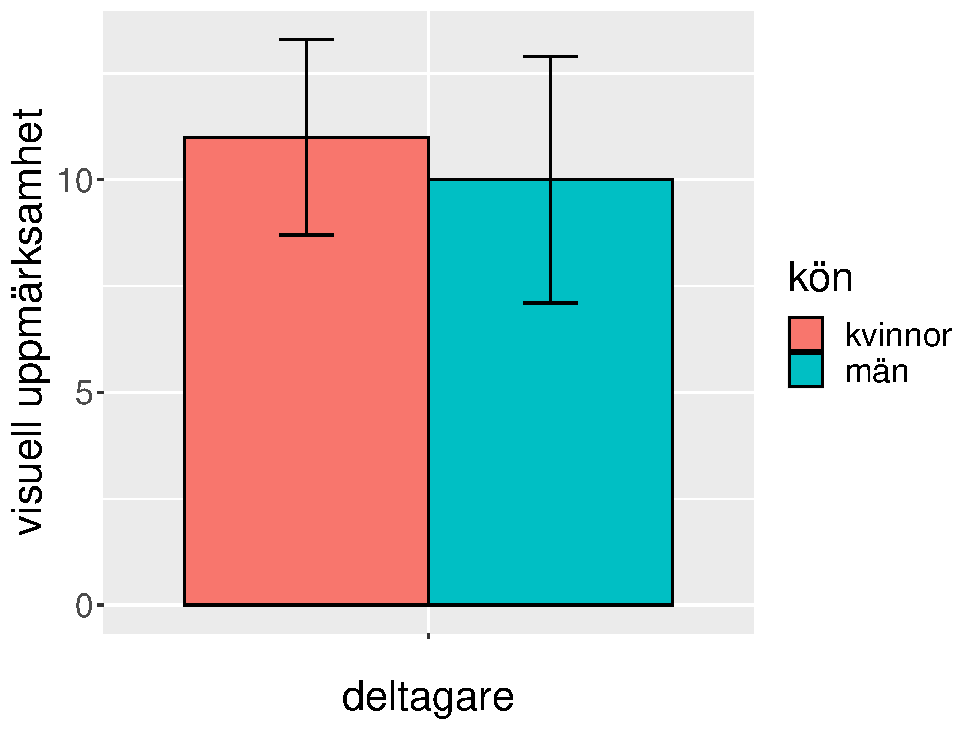
\includegraphics[width=0.8\linewidth]{scom-expb_files/figure-latex/fig-02-08-1-1-01-1} 

}

\caption{Beskrivande resultat eller deskriptiv statistik.}\label{fig:fig-02-08-1-1-01}
\end{figure}

I figuren kan vi som synes aggregera våra observationer genom att dela upp dem enligt någon demografisk variabel, i detta fall försöksdeltagarnas självrapporterade könstillhörighet. Denna typ av deskriptiv inledning till resultaten kan dock vara mer förekommande inom samhällsvetenskapliga experiment; inom andra ämnen kanske detta anses som lite onödigt, eftersom redovisningen inte direkt relaterar till hypotserna.

\hypertarget{sub08.1.2}{%
\subsection{Inferentiella resultat}\label{sub08.1.2}}

Efter den översiktliga presentationen av generella deskriptiva resultat, kommer vi så till själva kärnfrågan i vår tänkta studie: Vilken effekt hade det experimentella villkoret ``bild på auktoritetsperson'' på deltagarnas visuella uppmärksamhet på texten i Facebook posterna, jämfört med när samma text presenterades i kontrollvillkoret ``bild på okänd person''? Och vad hade samma experimentella manipulation för effekt på den andra beroende variabeln upplevd trovärdighet för samma texter? Som synes bygger dessa frågor vidare på de deskriptiva resultaten, men uppvisar ett annat sätt att dela upp empiriska observationer i olika grupper; i detta fall i kontroll- och behandlingsvillkor. När vi försöker besvara den kritiska frågan om det finns några skillnader mellan dessa två grupper med avseende på utfallsvariablerna, använder vi oss av s.k. statistisk inferens för att dra slutsatser om resultaten vid en fastställd nivå av sannolikhet.

\begin{figure}

{\centering 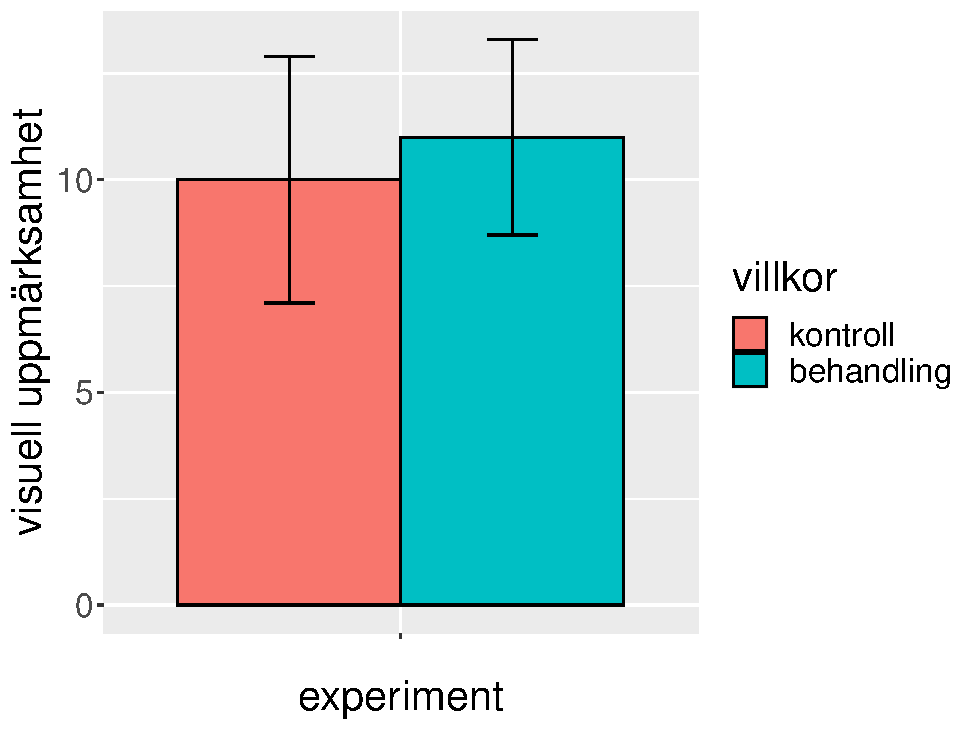
\includegraphics[width=0.8\linewidth]{scom-expb_files/figure-latex/fig-02-08-1-2-01-1} 

}

\caption{Inferentiella resultat.}\label{fig:fig-02-08-1-2-01}
\end{figure}

Ur detta diagram kan vi utläsa att deltagarna i genomsnitt ägnat mindre visuell uppmärksamhet åt Facebook-posterna i kontrollvillkoret jämfört med behandlingsvillkoret, men vi har fortfarande inget mått på tillförlitligheten i denna skillnad. För att kunna rapportera dessa inferentiella resultat av vårt experiment måste vi här gå tillbaka till hypoteserna som uppställdes i förarbetet till studien. Det kan vara en stor fördel att upprepa dessa hypoteser i resultaten, när vi rapporterar vilket stöd insamlade empiriska data ger till det förväntade utfallet. I vårt fall hade vi följande två hypotser, men för enkelhetens skull kommer vi i det följande bara att fokusera på den första.

\begin{itemize}
\item
  H1: Facebook-poster med bild på en auktoritetsperson kommer att orsaka mer visuell uppmärksamhet på posten jämfört med bilder som innehåller en neutral person.
\item
  H2: Facebook-poster med bild på en auktoritetsperson kommer att orsaka högre upplevd trovärdighet hos posten jämfört med bilder som innehåller en neutral person.
\end{itemize}

Ett enkelt men samtidigt robust sätt att testa dessa hypoteser är att göra ett s.k. t-test för varje hypotes. T-testet lämpar sig för situationer när vi har en kvantitativ beroende variabel och exakt två villkor som ska jämföras. Detta test jämför i princip medelvärdena i respektive grupp, med hänsyn tagen till bl.a. antal observationer (deltagare, försök, etc), samt observationernas fördelning och spridning (t.ex. standardavvikelse). För att kunna genomföra statistiska test behövs en nollhypotes, där vi antar att det inte finns någon skillnad mellan villkoren. Baserat på detta formulerar vi sedan hypotesen H1 om en skillnad mellan villkoren i en förväntad riktning (auktoritetsperson kommer att orsaka \emph{mer} visuell uppmärksamhet). Det sista steget som behövs är att vi antar en sannolikhetsnivå (s.k. alpha-nivå) att vi skulle observera de faktiska resultaten om nollhypotesen stämde bäst. En vanlig nivå är 0.05, vilket innebär att vi anser att uppmätta skillnader mellan villkoren är tillräckligt tillförlitliga om det är 5\% chans eller mindre att resultatet beror på slumpen, och 95\% chans eller mer att de beror på de experimentella villkoren\footnote{Här kan vi jämföra med naturvetenskapliga ämnen där standarden 5-\(\sigma\) eller ``fem sigma'' ibland används som gräns för att betrakta observationer som tillräckligt tillförlitliga. Fem sigma-nivån innebär att chansen är en på 3,5 miljoner att ett visst resultat orsakats slumpmässigt.}. Resultatet rapporteras i så fall som ``statistiskt signifikant''.

\begin{longtable}[]{@{}rrrrrr@{}}
\caption{\label{tab:tab-02-08-1-2-01}Inferentiella resultat.}\tabularnewline
\toprule
kontroll & behandling & t.värde & p.värde & frihetsgrader & effektstorlek\tabularnewline
\midrule
\endfirsthead
\toprule
kontroll & behandling & t.värde & p.värde & frihetsgrader & effektstorlek\tabularnewline
\midrule
\endhead
10 & 11 & 2.702 & 0.007 & 198 & 0.382\tabularnewline
\bottomrule
\end{longtable}

I detta exempel har vi antagit ett experiment med mellangruppsdesign och 100 deltagare i varje grupp. Medelvärdena för visuell uppmärksamhet var 10 och 11 sekunder i respektive grupp, och det statistiska testet visade ett t-värde på ca 2.7, och p-värdet visade sig vara under gänsen 0.05 som vi tidigare antog. Det positiva t-värde indikerar att riktningen i sambandet överensstämmer med det förväntade, dvs. att bilder med auktoritetsperson kommer att orsaka \emph{mer} visuell uppmärksamhet. Förutom detta t-test skulle man kunna tänka sig andra statistiska test för att undersöka de inferentiella resultaten av experimentet, bl.a. variansanalys (s.k. ANOVA) eller regressionsanalys (ifall vi hade velat kontrollera för särskilda variabler såsom kön eller ålder). Gemensamt för många av dessa test är att de följer NHST-modellen, och därmed ger oss ett probabilistiskt värde för hur sannolikt det vore att slumpmässigt observera de faktiska resultaten, vilket i sin tur ger oss möjligheter att dra slutsatser om huruvida experimentets behandlingsvillkor på ett kausalt sätt orsakat en viss effekt på deltagarna. Beyond p-value statistics \citep{trafimow2015editorial}.

Statistiska resultat, eller modellering, eller Inferentiell statistik, multivariat analys.. handlar om att redovisa resultat relativt något mått på tillförlitlighet. Detta kan också kallas ``statistiskt säkerställda'' resultat. The smaller the p-value, the stronger the evidence that you should reject the null hypothesis. In null hypothesis significance testing, the p-value is the probability of obtaining test results at least as extreme as the results actually observed, under the assumption that the null hypothesis is correct. - prediction vs.~fitting (meningsfulla modeller kan vara viktigare än prediktion, retro-fitting hypotheses). Här kommer nåt om causal inference.

\hypertarget{sec08.2}{%
\section{Diskussion}\label{sec08.2}}

Experimentets efterarbete är ingalunda klart i och med resultatrapporteringen som vi presenterade i föregående avsnitt. Även om vi med statistiska metoder kan visa att våra empiriska data ger mycket starkt stöd till de hypoteser som uppställts, så måste vi också visa att vi kan förhålla oss kritiska till dessa resultat, dvs. att vi förstår och redovisar svagheter i det genomförda experimentet, att vi undersökt möjliga felkällor, samt att vi kan föreslå förbättringar till experimentets design. Här kommer \emph{diskussionen} in som en ärlig, transparent och objektiv utvärdering av experimentets genomförande. Det finns ingen granskande forskare som förväntar sig att vi ska kunna åstadkomma ett perfekt experiment med begränsade resurser, och därför handlar det ofta om att vi som experimentledare tydligt redovisar och motiverar de avgränsningar och val som gjorts i studien.

Vi kan också tänka oss att diskussionen är den avslutande delen av studien där vi tittar tillbaka och sammanfattar alla delarna i experimentet, från forskningsfrågor, till hypoteser, vidare till genomförandet. Här skulle man kunna använda sig av en domstolsmetafor. Den experimentella studien är genomförd och nu står insamlat material och experimentdesign åtalad för att visa något. Bevis, evidens, circumstantial evidence, alias. Forskaren antar i så fall både rollen som åklagare (hypotes) och försvarsadvokat (nollhypotes). Diskussionen kan därför liknas vid en slutplädering, där all bevisning i målet sammanfattas innan domare och nämndemän avkunnar dom.

\hypertarget{sub08.2.1}{%
\subsection{Förväntade och faktiska resultat}\label{sub08.2.1}}

Ett av de viktigaste momenteten i diskussionen är sammanfatta vilket stöd våra empiriska data ger till de hypoteser vi uppställt, dvs. relationen mellan förväntade och faktiska resultat. Här kan det vara viktigt att poängtera att forskningsvärlden sällan talar om att hypoteser bekräftats eller besannats, utan man talar istället om hur resultaten \emph{stödjer} hypoteserna eller inte. Till syvende och sist kan inte vetenskapen ge slutgiltiga bevis om sanningen, utan den svarar på hur \emph{sannolikt} ett visst sakförhållande är, t.ex. effekten av ett experimentellt villkor på någon utfallsvariabel.

Även om experimentet uppvisar ett starkt signifikant resultat, kan effektstorleken vara ganska liten (avsnitt \protect\hyperlink{sub07.1.1}{7.1.1} förstudier). I resultaten från vårt exempel-experiment kom vi fram till att Facebook-poster med bild på auktoritetsperson medförde en statistiskt signifikant ökning av deltagarnas visuella uppmärksamhet på den tillhörande texten i samma post. Men samtidigt uppgav vi att det finns en 5\% chans att våra data är ett slumpmässigt extremfall, och att om experimentet upprepades så skulle denna effekt troligen inte visa sig igen. Denna risk att felaktigt finna stöd för sin hypotes kallas för typ I-fel (på engelska används det synonyma uttrycket ``false positive'').

\begin{longtable}[]{@{}lll@{}}
\caption{\label{tab:tab-02-08-2-1-01}Typ I- och Typ II-fel.}\tabularnewline
\toprule
Nollhypotesen.är\ldots{} & Sann & Falsk\tabularnewline
\midrule
\endfirsthead
\toprule
Nollhypotesen.är\ldots{} & Sann & Falsk\tabularnewline
\midrule
\endhead
Förkastas & Typ I-fel, Falsk positiv & Korrekt beslut, Sann positiv\tabularnewline
Förkastas inte & Korrekt slutsats, Sann negativ & Typ II-fel, Falsk negativ\tabularnewline
\bottomrule
\end{longtable}

Figuren ovan försöker illustrera hur resultaten av ett experiment kan förhålla sig till den faktiska omvärlden. Om vi i resultaten hittar den effekt vi har förväntat oss, så innebär ju detta att vi förkastar nollhypotesen, som säger att det inte finns någon effekt. Naturligvis hoppas vi (med 95\% sannolikhet) att detta resultat speglar verkligheten (s.k. ``true positive''). Om vi vill vara ännu mer säkra på att resultatet inte är ett extremt undantagsfall skulle vi kunna sänka den så kallade signifikansnivån från 0.05 till exemplevis 0.01. Vi skulle därmed kunna bli mer säkra på att undvika typ I fel, men samtidigt ökar då risken att vi istället hamnar i ett typ II-fel, vilket innebär att vi felaktigt antar nollhypotesen trots att det verkligen föreligger en effekt av behandlingen (s.k. ``false negative'').

Typ II-fel kan bero på felaktig power-analys, och kan i vissa fall åtgärdas genom att öka antalet deltagare och/eller försök (trials) i experimentet. Om vi har gjort en korrekt poweranalys och vi ändå inte ser en statistiskt säkerställd effekt av behandlingen kan vi vara mer säkra på att vi gör rätt när vi antar nollhypotesen (s.k. ``true negative''). Statistisk teori inom samhällsvetenskaperna handlar i mångt och mycket om att minimera båda dessa typer av fel, dock kan det vara så att i vissa kontexter kan endera feltypen vara mer accepterad, t.ex. i samband med en medicinsk cancerdiagnos är det bättre med typ I fel (överdetektion) än typ II fel (underdetektion).

\hypertarget{sub08.2.2}{%
\subsection{Alternativa förklaringar till resultat}\label{sub08.2.2}}

Om experimentet indikerar en signifikant kontrast mellan villkoren så försöker vi naturligvis försäkra oss om att detta är ett korrekt och representativt resultat. Ett sätt att göra detta är att använda s.k. multivariat analys, vilket tillåter oss att undersöka hur andra variabler än de experimentella villkoren bidrar till att förklara de effekter vi ser i resultaten. I detta fall kanske det inte räcker med ett t-test som vi visade tidigare, utan vi behöver utöka testet till en regressionsanalys. Har vi kontrollerat för alla viktiga variabler? Hur påverkar t.ex. deltagarnas individuella läshastighet resultaten för visuell uppmärksamhet på Facebook-posternas text? Kan vi anta att denna egenskap är jämnt fördelad mellan de experimentella villkoren, eller kan vi misstänka någon snedfördelning (bias)? Frågan vi ställer oss här handlar om ifall det finns andra variabler än de experimentella villkoren som driver fram studiens resultat.

För att kunna kontrollera alternativa förklaringar till resultaten måste vi tänka i förväg när vi designar experimentent. I detta skede är det relativt enkelt att lägga in extra frågor om deltagarnas attityder, kunskaper och beteenden, som det i efterhand är svårt eller omöjligt att ta reda på. En kompletterande metod att hantera konfunderande variabler och individuella skillnader mellan deltagare kan också vara genom att använda oss av en inomgruppsdesign (within-subjects) i experimentet. Kan vi dra slutsatser om kausala samband? Eventuellt ta upp moderator (counteracts, motverkar en effekt), mediator (förstärker en effekt), visa plot på interaktion, interaction plot.

\hypertarget{sub08.2.3}{%
\subsection{Kontextualisering och framtida forskning}\label{sub08.2.3}}

I de föregående avsnitten har vi försökt sammanfatta och kritisera de konkreta resultaten av experimentet. På detta sätt kan diskussionen likna slutpläderingen i en rättegång, där åklagaren försöker bevisa att en händelse har ägt rum, medan försvarsadvokaten kanske argumenterar för att det finns andra förklaringar till det som inträffat. När vi på ett övertygande sätt klarat av detta steg, brukar diskussionen avslutas med att vi försöker titta på studien i en lite större kontext. I detta sammanhang kan vi resonera kring hur pass väl resultaten kan generaliseras till en större befolkning, om de är representativa, samt hur vi bedömer studiens övergripande validitet och reliabilitet. Denna diskussion handlar delvis om kvalitet i kvantiativa studier, och det faller sig ganska naturligt att diskussionen öppnar sig för potentiella förbättringar av den genomförda studien.

Här är det också relevant att reflektera kring resultatens betydelse i en större samhällsvetenskaplig kontext, samt det genomförda experimentets bidrag till befintlig forskning inom ett specifikt forskningsfält och angränsande fält. Som vi diskuterat redan i förarbetet, så måste vi ha studerat tidigare forskning väldigt ingående för att ha en möjlighet att bidra till detta forskningsfält. Här kan diskussionen med fördel anknytas till studiens forskningsfråga (eller ``research question''):

\begin{itemize}
\tightlist
\item
  RQ1: Hur påverkar bildinnehållet i sociala medier-poster användarnas beteenden och attityder?
\end{itemize}

Efter att ha genomfört vårt exempel-experimentet är vi nu i en situation där vi kan ge ett tentativt svar på denna forskningsfråga, samt eventuellt också utveckla hur dessa nya forskningsrön skulle kunna tillämpas praktiskt inom exempelvis kommunikationsyrken. Om resultaten levererar svar på studiens konkreta målsättningar, så kan diskussionen alltså införliva den lite mer utmanade frågan om hur resultaten leverar gentemot studiens övergripande syfte.

\newpage

\hypertarget{part-del-3}{%
\part{Del 3}\label{part-del-3}}

\hypertarget{del-3}{%
\chapter*{Del 3}\label{del-3}}
\addcontentsline{toc}{chapter}{Del 3}

I denna del av boken följer vi utvecklingen och genomförandet av ett samhällsvetenskapligt experiment.

\hypertarget{chap09}{%
\chapter{Kapitel}\label{chap09}}

some line

  \bibliography{book.bib,packages.bib}

\end{document}
